\documentclass[]{emulateapj}

\usepackage{hyperref} % hyperref works too
\urlstyle{same}  % (sf also works, for something more subtle than tt)
\usepackage{amsmath}

\usepackage{mathrsfs}
%\usepackage{natbib}

\usepackage[]{units} % Provides \nicefrac

\usepackage{threeparttable}
\usepackage{multirow}

\usepackage{soul}

\renewcommand{\textfraction}{.1}
\renewcommand{\floatpagefraction}{.9}
%\makeatletter% Set distance from top of page to first float
%\setlength{\@fptop}{5pt}
%\makeatother

\usepackage{ulem}
%\usepackage[total={6.5in,9.0in},
%top=1.75in, left=1.0in, 
%includefoot]{geometry}       % See geometry.pdf to learn the layout options. There are lots.

%\geometry{letterpaper}                   		% ... or a4paper or a5paper or ... 
%\usepackage[parfill]{parskip}    		% Activate to begin paragraphs with an empty line rather than an indent
\usepackage{graphicx}				% Use pdf, png, jpg, or eps� with pdflatex; use eps in DVI mode
								    % TeX will automatically convert eps --> pdf in pdflatex		
\usepackage{dblfloatfix}

\setlength{\textfloatsep}{4pt plus 1.0pt minus 2.0pt}

\def\etal{{\textit{et al.} }}
\def\eg{{\textit {e.g. }}}

\begin{document}
\title{Following the Cosmic Evolution of Pristine Gas II: The search for Pop III-Bright Galaxies }
\shorttitle{The search for Pop III-Bright Galaxies}
%\author{Richard Sarmento\altaffilmark{1} and Evan Scannapieco\altaffilmark{1},}
\author{Richard Sarmento, Evan Scannapieco and Seth Cohen}
%\altaffiltext{1}{School of Earth and Space Exploration,  Arizona State University, P.O. Box 871404, Tempe, AZ, 85287-1404}
\affil{School of Earth and Space Exploration,  Arizona State University, P.O. Box 871404, Tempe, AZ, 85287-1404}

%%%%%%%%%%%%%%
%%%%%%%%%%%%%%
% Three paragraphs, entitled respectively ?Aims?, ?Methods?, and ?Results?, are
% mandatory. When appropriate, the structured abstract may use an introductory paragraph entitled ?Context?,
% and a final paragraph entitled ?Conclusions?.
% The objectives of the paper are defined in ?Aims?, the methods of the investigation are outlined in
% ?Methods?, and the results are summarized in ?Results?. The heading ?Context? is used when needed to
% give background information on the research conducted in the paper, and ?Conclusions? can be used to
% explicit the general conclusions that can be drawn from the paper.
% Note that the use of structured abstracts in A&A articles and Letters is not mandatory. Authors who
% prefer the traditional form are invited to implicitly follow the logical structure indicated above.
\begin{abstract}
We use a large scale cosmological simulation, augmented with a new subgrid model of turbulent mixing, to follow the cosmological evolution of the first galaxies and to accurately model their fraction of Population III (Pop III) stars. We model the flux from these early galaxies and present theoretical predictions that will help guide deep surveys and the search for Pop III stars at $8 \le z \le 16$. We generate rest-frame ultraviolet (UV) luminosity functions (LFs) for our galaxies and find that they are in reasonable agreement with both the limited observations at $z > 8$ as well as the latest extrapolations of the Schechter function faint-end slope out to $z = 16$. We find galaxies brighter than $m_{\rm UV, AB} \le 31.4$ mag throughout our redshift range and predict detections in James Webb Space Telescope (JWST) Near Infrared Camera (NIRCam) filters out to $z=15$ for filter redder than 2.77 $\mu$m. To aid the search for Pop III stars, we identify `Pop III-bright' galaxies: galaxies with at least 75\% of their flux coming from young, hot stars. We find that 40\% of galaxies brighter than $m_{\rm UV, AB} = 31.4$ mag are Pop III-bright over the redshift range $13 \le z \le 14$ with about 20\% Pop III-bright at $z=15$. While Pop III-bright galaxies are not detectable at $z=16$ at this magnitude limit, we find 90\% of galaxies at $z=16$ are Pop III-bright with $m_{\rm UV, AB} \le 33$ mag.
\end{abstract}

\keywords{cosmology: theory, early universe -- galaxies: high-redshift, evolution -- stars: formation, Population III -- luminosity function -- turbulence}

%\date{}	% Activate to display a given date or no date  

%%%%%%%%%%%%%%
%%%%%%%%%%%%%%
\section{Introduction}
Finding and characterizing the first galaxies is the next frontier in observational astronomy. In particular, understanding the distribution, luminosities, and spectral energy densities (SEDs) of high redshift galaxies will undoubtedly revise our understanding of the nature of the first stars. Conversely, the characteristics of the first stars play a major role in the detectability of these early galaxies \citep{2004ARA&A..42...79B}. 

The first stars formed from pristine gas with metallicity $Z\approx 0$ that collapsed within mini-halos with total masses of $\sim 10^{5}-10^{6} M_{\odot}$ \citep{2002Sci...295...93A,2003ApJ...592..645Y}. The shallow gravitational potentials of these early proto-galaxies was only able to heat the in-falling gas to $\approx 10^{4}\, K$ -- where cooling via molecular hydrogen was the primary avenue to star formation \citep{2002ApJ...564...23B}. The relatively inefficient cooling by $H_{2}$ likely suppressed cloud fragmentation leading to a generation of massive, yet short-lived, metal-free stars \citep{2002Sci...295...93A, 2002A&A...382...28S}. %While the high-intensity UV flux from such stars played only a minor role in reionization \citep{2013MNRAS.429L..94P}, this radiation likely suppressed further star formation in these early mini-halos. 

By definition, the first Pop III stars must have formed in the primordial gas. However, they also form in gas with metallicity below a critical threshold, $Z_{\rm crit}$. The exact value of the threshold depends on whether the dominant cooling channel for the gas is the fine-structure lines of metals or via dust emission  \citep{2003Natur.422..869S, 2003Natur.425..812B,2005ApJ...626..627O}. While the value is poorly constrained, it is believed to be in the range  $10^{-6} < Z_{\rm crit} < 10^{-3} Z_{\odot}$. 

Theoretical studies suggest that these metal-free stars could be observed today, if their initial mass function (IMF) extended to low masses \citep{2006ApJ...653..285S, 2006ApJ...641....1T, 2007ApJ...661...10B,2010MNRAS.401L...5S,2015MNRAS.447.3892H,2016arXiv160200465I}. However, no one has yet observed a Pop III star in or near the Galaxy \citep{2002Natur.419..904C, 2004A&A...416.1117C, 2006ApJ...639..897A,2005Natur.434..871F, 2007ApJ...670..774N,2011Natur.477...67C,2014Natur.506..463K,2015Natur.527..484H}. High-redshift observations have yielded candidates for Pop III stellar populations \citep{2002ApJ...565L..71M, 2004ApJ...617..707D, 2006Natur.440..501J, 2007MNRAS.379.1589D, 2008ApJ...680..100N, 2012ApJ...761...85K, 2013A&A...556A..68C} including a controversial z = 6.6 galaxy analyzed by \cite{2015ApJ...808..139S} that displays HeII $\lambda$1640 emission -- a likely indicator of the hard-ultraviolet (UV) spectrum produced by Pop III stars \citep{2001ApJ...550L...1T}. However, to date, there has not been a confirmed observation of a galaxy dominated by the flux from Pop III stars \citep{2017MNRAS.468L..77P, 2016arXiv160900727B}.  

%Another key factor controlling the formation of Pop III stars is the rate at which gas with $Z < Z_{\rm crit}$ -- the pristine gas fraction -- is polluted above this critical metallicity \citep{2007ApJ...654L..29P, 2010ApJ...716..510G, 2012JFM...700..459P, 2013ApJ...775..111P, 2013IAUS..295....3B, 2014MmSAI..85..202B, 2015MNRAS.451.1190R}. The relevant physics here is properly understanding -- and then modeling -- the rate at which the pristine gas fraction decays as a function of time and space. In turn, the decay rate is governed by the frequency at which stars deposit new pollutants into the surrounding gas and on how large-scale motions transport those pollutants. 
%
%The pollution of pristine gas is also dependent on the small-scale turbulent mixing of metals which typically takes place at scales far below those typically modeled in cosmological simulations \citep{2013ApJ...771...81R, 2015ApJ...807L..12O}. This discrepancy in scales -- and its effects on the metallicity of star-forming gas -- has typically gone unaddressed in cosmological simulations. 

%% Transition to LF -- Purely pop iii galaxies are going to be hard to observe... We need to understand the LF to predict number densities.
This may change in the near future. The soon-to-launch James Webb Space Telescope (JWST) is poised to greatly expand our understanding of the high-redshift universe and possibly detect the first galaxies dominated by Pop III flux. Using JWST astronomers will be able to amass galaxy catalogs out to $z\approx 10$ and probe the era of the first galaxies \citep{2016jwst}. This will likely require observations to $z\gtrsim 12$  - a mere 370 Myr after the Big Bang -- and beyond. What types of galaxies is JWST likely to discover? How are they distributed?  We attempt to answer these question by characterizing simulated galaxy populations at high redshift.

The evolution of the galaxy luminosity function (LF) is a useful tool in this endeavor since it describes galaxy density as a function of luminosity across cosmic time. Utilizing Hubble Space Telescope (HST) observations, astronomers have been able to amass galaxy catalogs out to $z=8$ and place some initial constraints on galaxy populations out to $z\approx11$ \citep{2017arXiv170204867I, 2016PASA...33...37F, 2015ApJ...803...34B, 2016ApJ...816...46M, 2015MNRAS.450.3032M, 2013ApJ...762...32C, 2013ApJ...773...75O}. While a lot of progress has been made, the latest work at $z>8$ is hampered by small number statistics and completeness uncertainties \citep{2017ApJ...835..113L, 2015ApJ...808..104O, 2015ApJ...814...69A}. The uncertainty in the rate of decay of the LF at $z>8$ \citep{2013ApJS..209....3K, 2014ApJ...795..126B}  is the concern here. If the LF falls off too quickly, as characterized by $M^{*}$ -- the absolute magnitude where galaxy counts experience an exponential decay, there will not be much for JWST to see beyond $z \approx 10$.

Several groups have used large scale cosmological simulations and analytic models to investigate galaxy formation, the high-$z$ LF and galaxy assembly \citep{2017arXiv170102749B, 2016ApJ...816...46M, 2015ApJ...807L..12O}. Others have used simulation to explore the transition between Pop III and Population II (Pop II) star formation \citep{2003ApJ...589...35S, 2007MNRAS.382..945T, 2007ApJ...654...66O, 2010ApJ...712..435T, 2010MNRAS.407.1003M, 2011ApJ...740...13Z, 2012ApJ...745...50W, 2013ApJ...773..108C, 2013MNRAS.428.1857J, 2013ApJ...775..111P,2014MNRAS.440.2498P}.  In this work we use simulation and our new model of Pop III star formation at sub-grid scales to present theoretical predictions for deep galaxy surveys. 

We make use of the work in \cite{2017ApJ...834...23S} enabling us to model turbulent mixing at subgrid scales and to track the pollution of the pristine gas in our simulation. By predicting the evolution of the pristine gas we can estimate the fraction of Pop III stars created in regions that would otherwise be considered polluted above $Z_{\rm crit}$.  Determining the density and evolution of Pop III stars is key to characterizing the luminosity of early galaxies \citep{2002A&A...382...28S}.  Pop III stars should lend unique observational characteristics to galaxies dominated by their flux \citep{2015MNRAS.450.2506V}.    

Our approach uses a customized version of \textsc{ramses} \citep{2002A&A...385..337T}, a cosmological adaptive mesh refinement (AMR) simulation. Using \textsc{ramses}, we follow galaxy formation from the dawn of star formation, at $z\approx 21$, to $z=7$. We generate rest-frame UV ($1500\AA$) luminosity functions for our galaxies, as well as filter-fluxes for a set of JWST Near InfraRed Camera (NIRCam) and two HST filters, across a redshift range that should be within reach of JWST. Moreover, using our unique capability to track the rate of subgrid metal pollution, we trace the formation of Pop III stars in these early galaxies and model their impact on the galaxies' flux. In doing so we identify a fraction of galaxies, across a range of redshifts, that have a significant fraction of Pop III flux from young massive stars.  We predict their prevalence in the early universe where they should be detectable by the hard-UV radiation that gives rise to HeII $\lambda$1640 emission. Additionally, we characterize the evolution of the galaxy mass-metallicity relation in the early universe and briefly discuss the masses of early galaxies dominated by Pop III stars.

The work is structured as follows.  In \S2 we describe our methods, including a brief discussion of our implementation of the subgrid model of metal pollution and our \textsc{ramses} cosmological model. In \S3 we describe our results with a focus on the luminosity function of high-redshift galaxies and an analysis of the fraction of Pop III flux emitted by them. Conclusions are discussed in \S4. Throughout this paper, we adopt the following cosmological parameters: $\Omega_{\rm M} = 0.267$, $\Omega_{\Lambda} = 0.733$, $\Omega_{\rm b} = 0.0449$, $h = 0.71$, $\sigma_8 = 0.801$, and $n = 0.96,$  where $\Omega_{\rm M}$, $\Omega_{\Lambda}$, $\Omega_{\rm b}$ are the total matter, vacuum, and baryonic densities, in units of the critical density, $h$ is the Hubble constant in units of 100 km/s, $\sigma_8$ is the variance of linear fluctuations on the 8 $h^{-1}$ Mpc scale, and $n$ is the ``tilt" of the primordial power spectrum \citep{2011ApJS..192...16L}. Finally, for this work, we have defined $Z_{\rm crit}= 10^{-5} Z_{\odot}$. 
%cosmology 7-year WMAP ?CDM+SZ+LENS best fit (Komatsu et al. 2011)

%%%%%%%%%%%%%%
%%%%%%%%%%%%%%
\section{Methods}

For this study we make use of \textsc{ramses} \citep{2002A&A...385..337T}, a cosmological adaptive mesh refinement (AMR) simulation code that uses an unsplit second-order Godunov scheme for evolving the Euler equations across the range of resolution elements (cells). \textsc{ramses} tracks cell-centered variables, which are interpolated to the cell faces for flux calculations. Flux between cells is computed using a Harten-Lax-van Leer-Contact Riemann solver \citep{1979JCoPh..32..101V,1988SJNA...25..294E} and the code is capable of advecting any number of these scalar quantities, that are scaled by the cell's mass-density, across simulation cells.  Self-gravity is solved using the multigrid method \citep{GT2011} along with the conjugate gradient method for levels $\ge 12$ in our simulation. \textsc{ramses} creates star particles (SP) in regions of over-dense gas, each of which represents thousands of solar masses of individual stars. Each such star particle is tagged with a scalar, $\overline Z_{\star}$, representing the average metallicity of the medium from which it was born, as well as a scalar, $P_{\star}$, that indicates the mass-fraction of the SP with $Z_{\star} < Z_{\rm crit}$. This mass-fraction represents Pop III stars. The pristine fraction, $P$, for the gas and $P_{\star}$ for star particles is described below.

%%%%%%%%%%%%%%
\subsection{The Pristine Fraction and the Corrected Metallicity}
In order to more accurately model the fraction of Pop III stars created throughout cosmic time, we track new, metallicity-related quantities for both the gas and SPs as described in detail in \cite{2017ApJ...834...23S}. Only an extremely high-resolution simulation would be able to track the metallicity of the gas at star-forming scales. Since this is currently not feasible in a cosmological simulation, we track the \textit{pristine gas mass-fraction}, $P$, that models the mass-fraction of gas with $Z < Z_{\rm crit}$ in each simulation cell. This allows us to model the process of metal mixing by quantifying the amount of pristine gas within each cell as a function of the cell's size, turbulent velocity, sound speed, and average metallicity, $\overline Z$. 

Figure \ref{fig:exz} depicts the problem we are addressing. Using a single scalar, simulation cells are only able to model an average metallicity across their volume. In reality, the metals may have only had time to mix within a fraction of the cell and are therefore concentrated in a fraction of the cell's volume. Modeling the decay of the pristine gas fraction allows us to track the formation of Pop III stars, as a mass fraction of all stars created, even in cells with an average metallicity above critical.  This fraction is captured in the scalar $P_{\star}$. Furthermore, by knowing the average metallicity, $\overline Z$ (or $\overline Z_{\star}$ for SPs), and the pristine gas fraction, $P$, we can better model the metallicity of the polluted fraction of gas in which the SPs are created. More explicitly, since $\overline Z$ represents the average metallicity of a parcel of gas, and the polluted fraction, $f_{\rm pol} \equiv 1-P$, models the fraction of gas that is currently polluted with metals, we can use the value of $f_{\rm pol}$ to predict the enhanced, or corrected, metallicity ($Z > \overline Z$) of the polluted fraction of gas in each simulation cell. This enables us to more accurately model the metallicity of the polluted fraction of stars, by mass, created in such cells.  The metallicity of the polluted fraction of gas, and hence the metallicity of SPs formed in the polluted fraction, is:

\begin{equation}\label{eq:zcorr}
\begin{aligned}
Z = \frac{\overline Z} {f_{\rm pol}},
\end{aligned}
\end{equation}
with $Z_{\star}$ similarly capturing the corrected metallicity of star particles. As expected, when $f_{\rm pol} = 1$ the corrected metallicity is the cell's average metallicity.

The metallicity of the polluted fraction of gas as described by Eqn.~\ref{eq:zcorr} is only precise when all of the metals are contained in the polluted fraction. This is true only in regions where the pristine gas is first polluted by Pop III supernova (SN). However, it is possible for some of the metals to be distributed in the pristine gas fraction defined as $0 \le Z < Z_{\rm crit}$. As discussed in \cite{2017ApJ...834...23S} this results in a small uncertainty in the resulting corrected metallicity of our SPs which we will ignore in this work. However, we can easily bound the correction to metallicity. While equation (\ref{eq:zcorr}) represents the upper bound, the lower bound on the correction is 

\begin{equation}\label{eq:lowerlim}
\begin{aligned}
Z = \frac{\overline Z - Z_{\Bbb {P}} P }{f_{\rm pol}},
\end{aligned}
\end{equation}
where $Z_{\Bbb {P}} = 10^{-5} Z_{\odot}$ is the upper limit on the metallicity of the pristine gas. If the pristine fraction has $Z_{\Bbb {P}}=0$, as it would when polluting the primordial gas, we recover equation (\ref{eq:zcorr}).  Even when considering this uncertainty, the corrected metallicity, $Z$, allows us to more accurately model the metallicity of our gas and SPs than would be possible using the average metallicity alone. 

Lastly we note that we do not create polluted stars when $f_{\rm pol} < 10^{-5}$. In this case, we assume all stars formed in the cell are Pop III since only a tiny fraction of the cell is polluted with metals.

\begin{figure}[h]
\begin{center}
\begin{tabular}{cc}
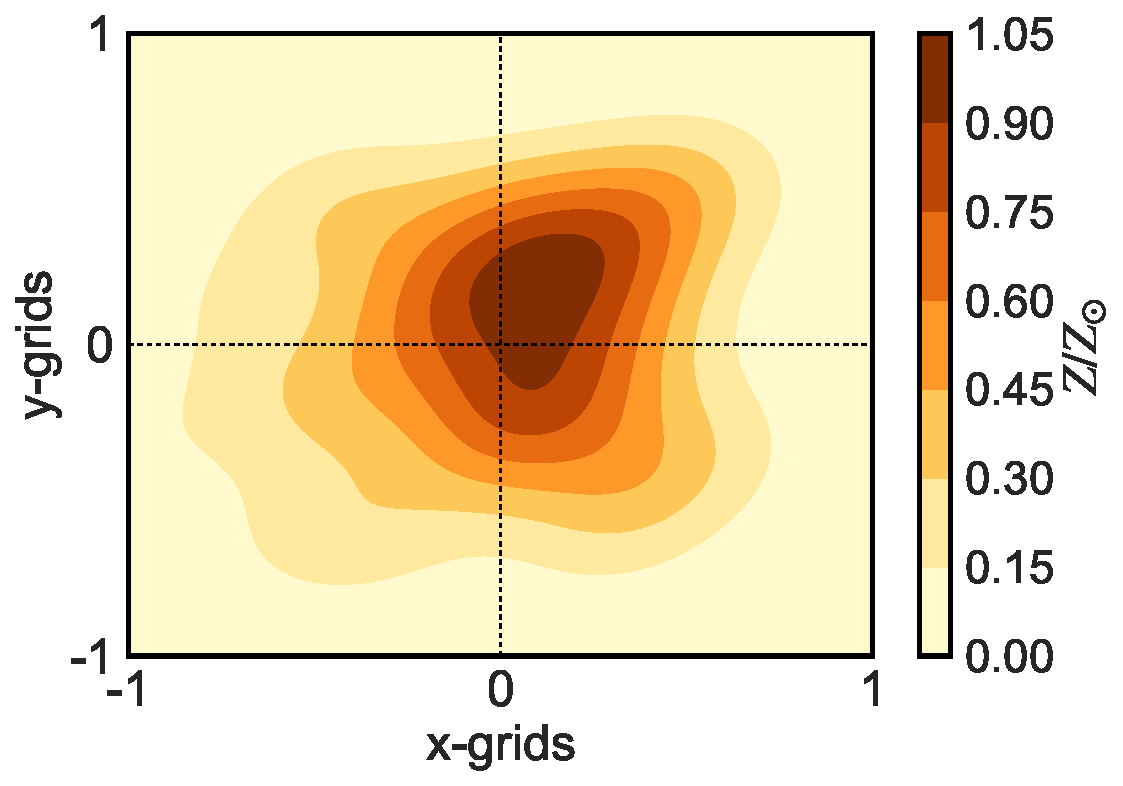
\includegraphics[width=1\columnwidth]{./exampleZ}
\end{tabular}
\caption{An example (2D) distribution of metal concentrations across a set of AMR cells. While the average metallicity, $\overline{Z}$, across these four cells is greater than $Z_{\rm crit}$, there are clearly regions that are still pristine. We track a new scalar, $P$, in each AMR cell to quantify the fraction of gas with $Z < Z_{\rm crit}$. In conjunction, $P$ and $\overline{Z}$ allow us to better model the actual metallicity of the polluted fraction (as described in the text).}
\label{fig:exz}
\end{center}
\end{figure}

\begin{figure*}[h]
\begin{center}
\begin{tabular}{cc}
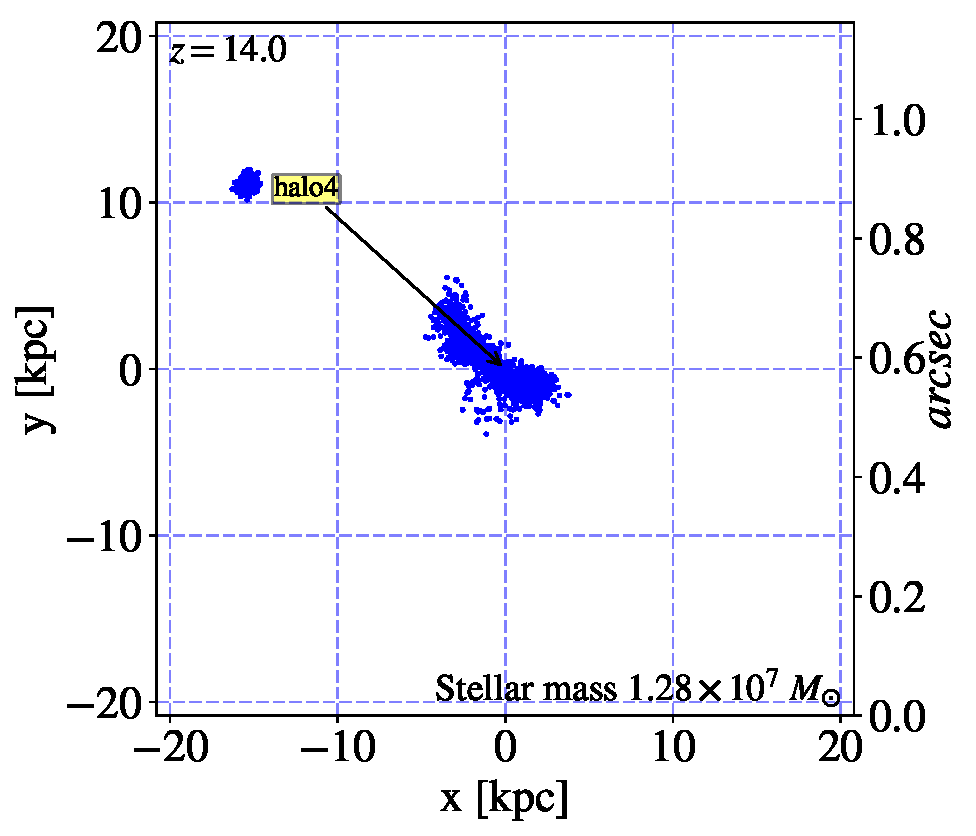
\includegraphics[width=1\columnwidth]{./SP-galaxy_z_14_0_3} &
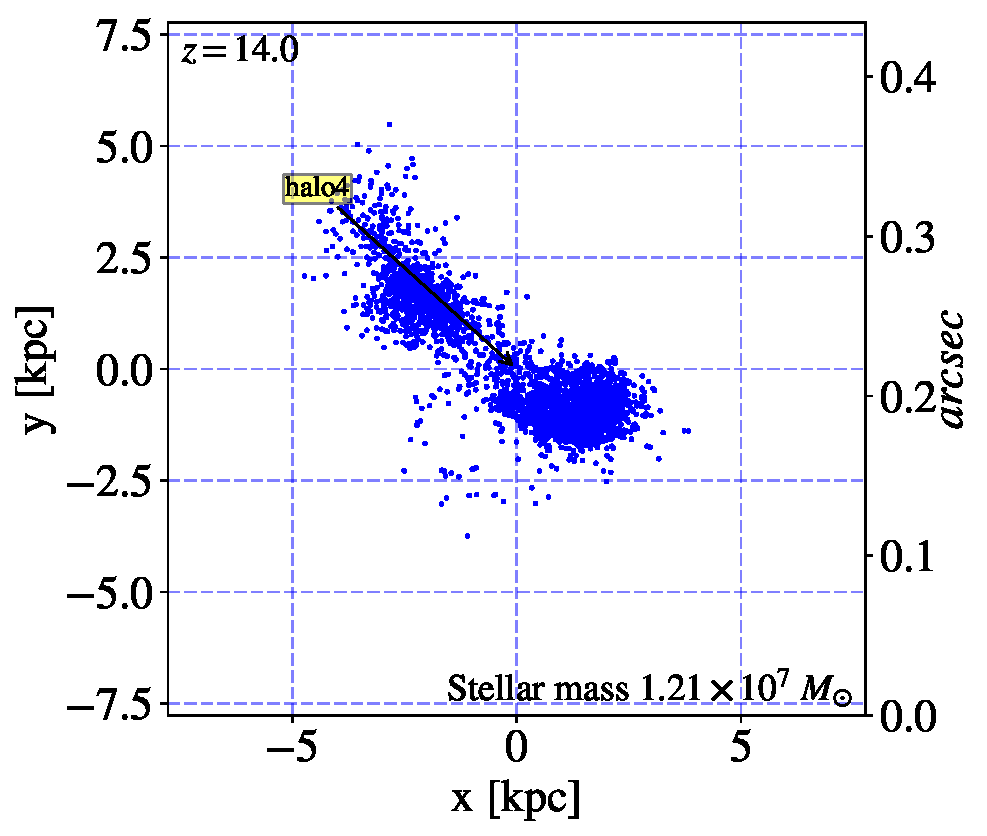
\includegraphics[width=1\columnwidth]{./HOP-galaxy_z_14_0_3} \\
\includegraphics[width=1\columnwidth]{./SP-galaxy_z_10_0_7} &
\includegraphics[width=1\columnwidth]{./HOP-galaxy_z_10_0_7} \\
\end{tabular}
\caption{Scatter plots of high-redshift galaxies in our simulation. Blue points are SP locations relative to the center of the located halo (coordinate 0,0). The images on the left depict the SP-HOP-halos found by our modified SP-based algorithm. As can be seen, more than one observationally identifiable galaxy is plotted within the radius depicted (left). On the right, we have used our post-processing algorithm to correctly identify the larger of the two galaxies in the original field. The smaller galaxy was also identified but not depicted independently in this figure. The scale is comoving kpc and the total mass of the galaxy is identified in the lower-right of each plot. The scale on the right axes indicates the size of the field in arcseconds.}
\label{fig:galaxs}
\end{center}
\end{figure*}

%%%%%%%%%%%%%%
\subsection{Halo Finding}
We use a modified version of HOP \citep{1998ApJ...498..137E} to find star-forming regions in the simulation volume, at each redshift of interest. The standard version of HOP, distributed with \textsc{ramses}, uses the simulation's dark matter (DM) particles to find collapsed objects. However, due to the large number of DM particles in our simulation ($\approx 10^9$) and a limitation in FORTRAN's ability to write very large files, it was much more efficient (in terms of both run-time and disk space) to use the SPs to find the galaxies analyzed for this study. Our SP-based HOP (SP-HOP) algorithm finds all of the star-forming regions in our simulation, although we only analyze those with masses above $10^{5} M_{\odot}$.

Many of the more massive objects found by SP-HOP consist of more than one observationally distinguishable galaxy. Hence we post-processed the halos as follows: For each SP-HOP halo we compute a mass, in stars, within a 3 kpc (comoving) sphere centered on the halo's coordinates. This typically corresponds to the core of the most massive galaxy in the field (if there is more than one). Next, we iteratively compute the mass in larger concentric spheres about this core. At each step we increase the radius by $10^{-1}$ arcsec -- converted to a proper distance (in kpc) at the galaxy's redshift. By using a redshift-dependent step-size based on the observational reference frame we can roughly determine the boundaries of our galaxies assuming, as is possible with the HST, that objects on the order of 0.1 arcsec apart are distinguishable. We continue increasing the radius until the fractional change in enclosed mass is less than 1 part in $10^{4}$. Specifically, when $\nicefrac{\Delta M_{\rm enc,i}}{M_{\rm enc,i}} < 10^{-4}$ we consider the current radius to be the radius of a single galaxy. This process results in galaxies with radii much smaller than a typical DM-based virial radius. Again, this is an advantage since DM halos may have more than one distinguishable galaxy within their virial radii.
Figure~\ref{fig:galaxs} depicts a set of un-reprocessed SP-HOP-halos (left) and resolved galaxies (right) that result from using this procedure. The approach ensures we do not over-represent bright objects, by considering multiple galaxies as one, when computing their luminosities.

To ensure that we capture the faint-end of the luminosity function, ignoring simulation resolution effects for now, we also locate and analyze the `missing' galaxies in our simulation: i.e. - those that may have been orphaned by the procedure described above. To accomplish this we collect the locations of all SP, at each redshift, that are \textit{not} within the previously computed radii of SP-HOP galaxies. This results in a set of orphaned SP.  Next, we select a star particle from this orphan list and locate all SPs within a 2 kpc, comoving, radius. If there are none, we assume the star is a galactic outlier and ignore it for the current iteration and select another star. Given a collection of SPs within 2 kpc, we compute the center-of-mass of this set and use this new location with our expanding sphere method to find the extent of the galaxy. If the resulting object has $M_{\rm G} > 10^5\;M_{\odot}$, its center-of-mass location and radius are added to the list of galaxies and stored; otherwise it is ignored. In either case, all of the object's SPs are then removed from the orphan list and the procedure is repeated until all SPs have been processed. 

Figure~\ref{fig:halos} depicts the results of our halo finding approach for $z=15$ \& $12$; approximately 276 and 377 Myr after the big bang, respectively. In this figure SPs are indicated by blue dots and the location of galaxies by red circles. The size of the circles correspond to the stellar mass of the galaxy with the key in the upper right corner indicating the circle-size for an average-mass galaxy at the redshift depicted.

\begin{figure*}[h]
\begin{center}
\begin{tabular}{cc}
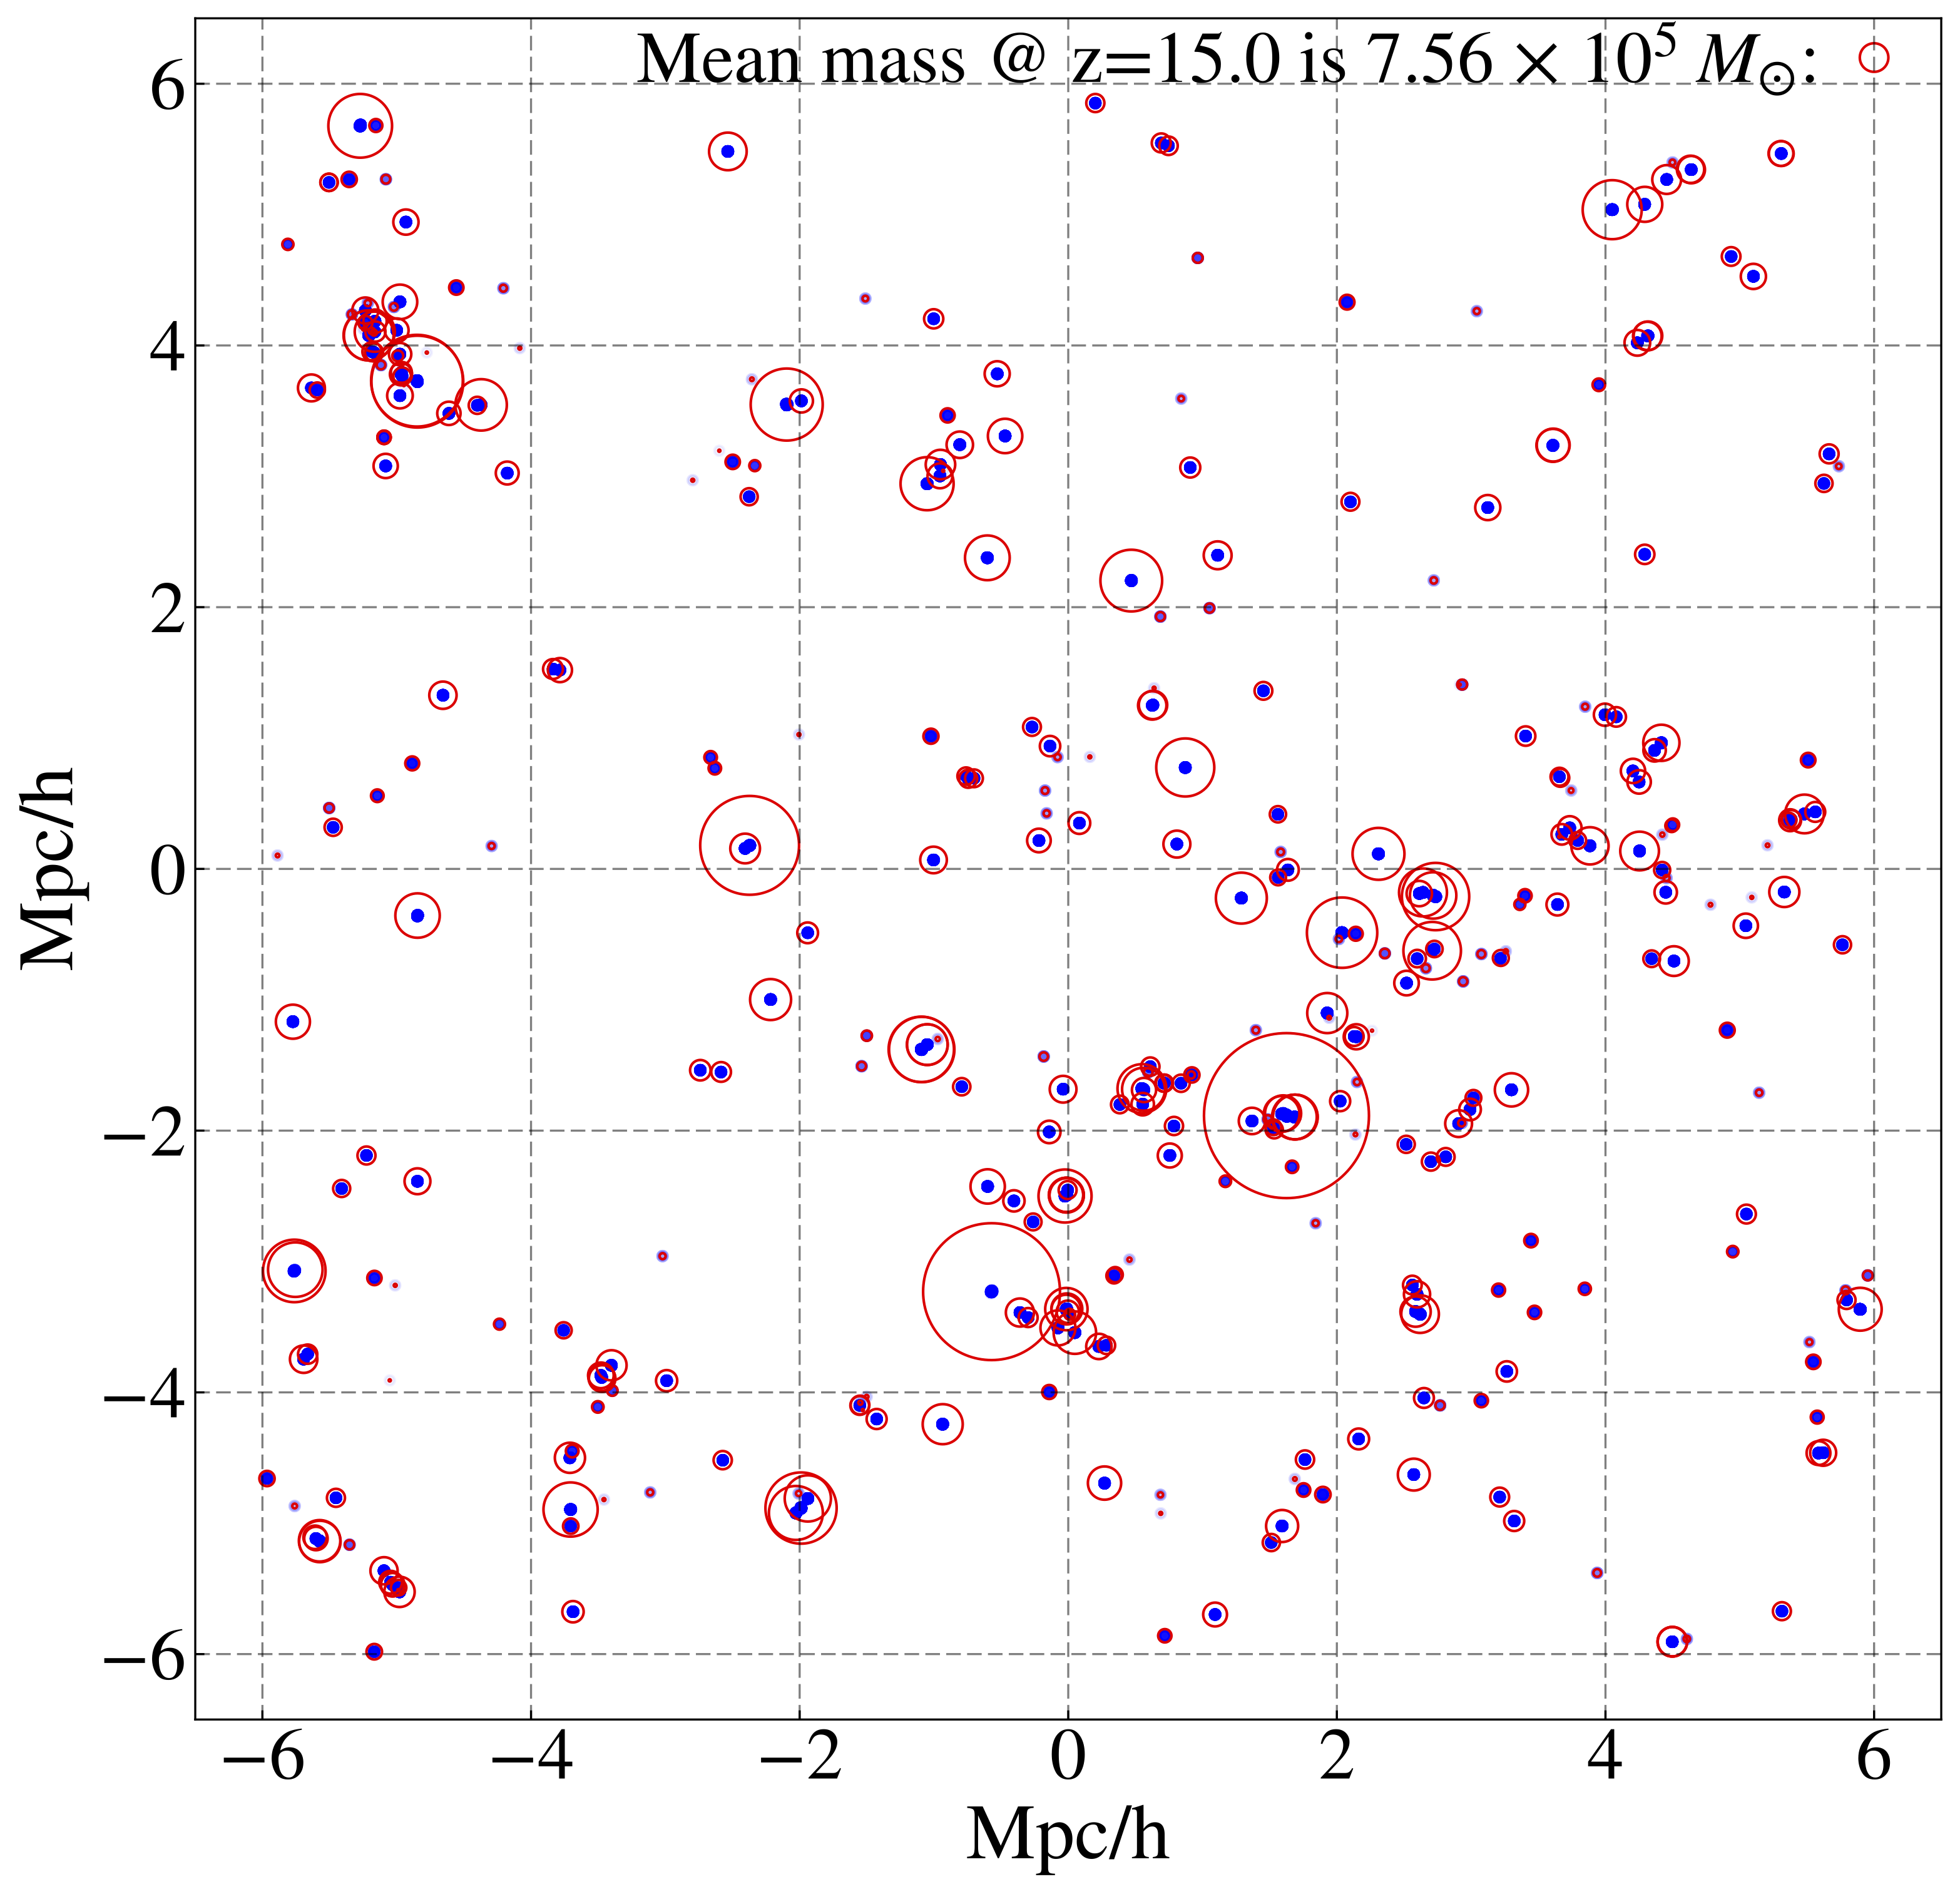
\includegraphics[width=1\columnwidth]{./AllHalos_150} &
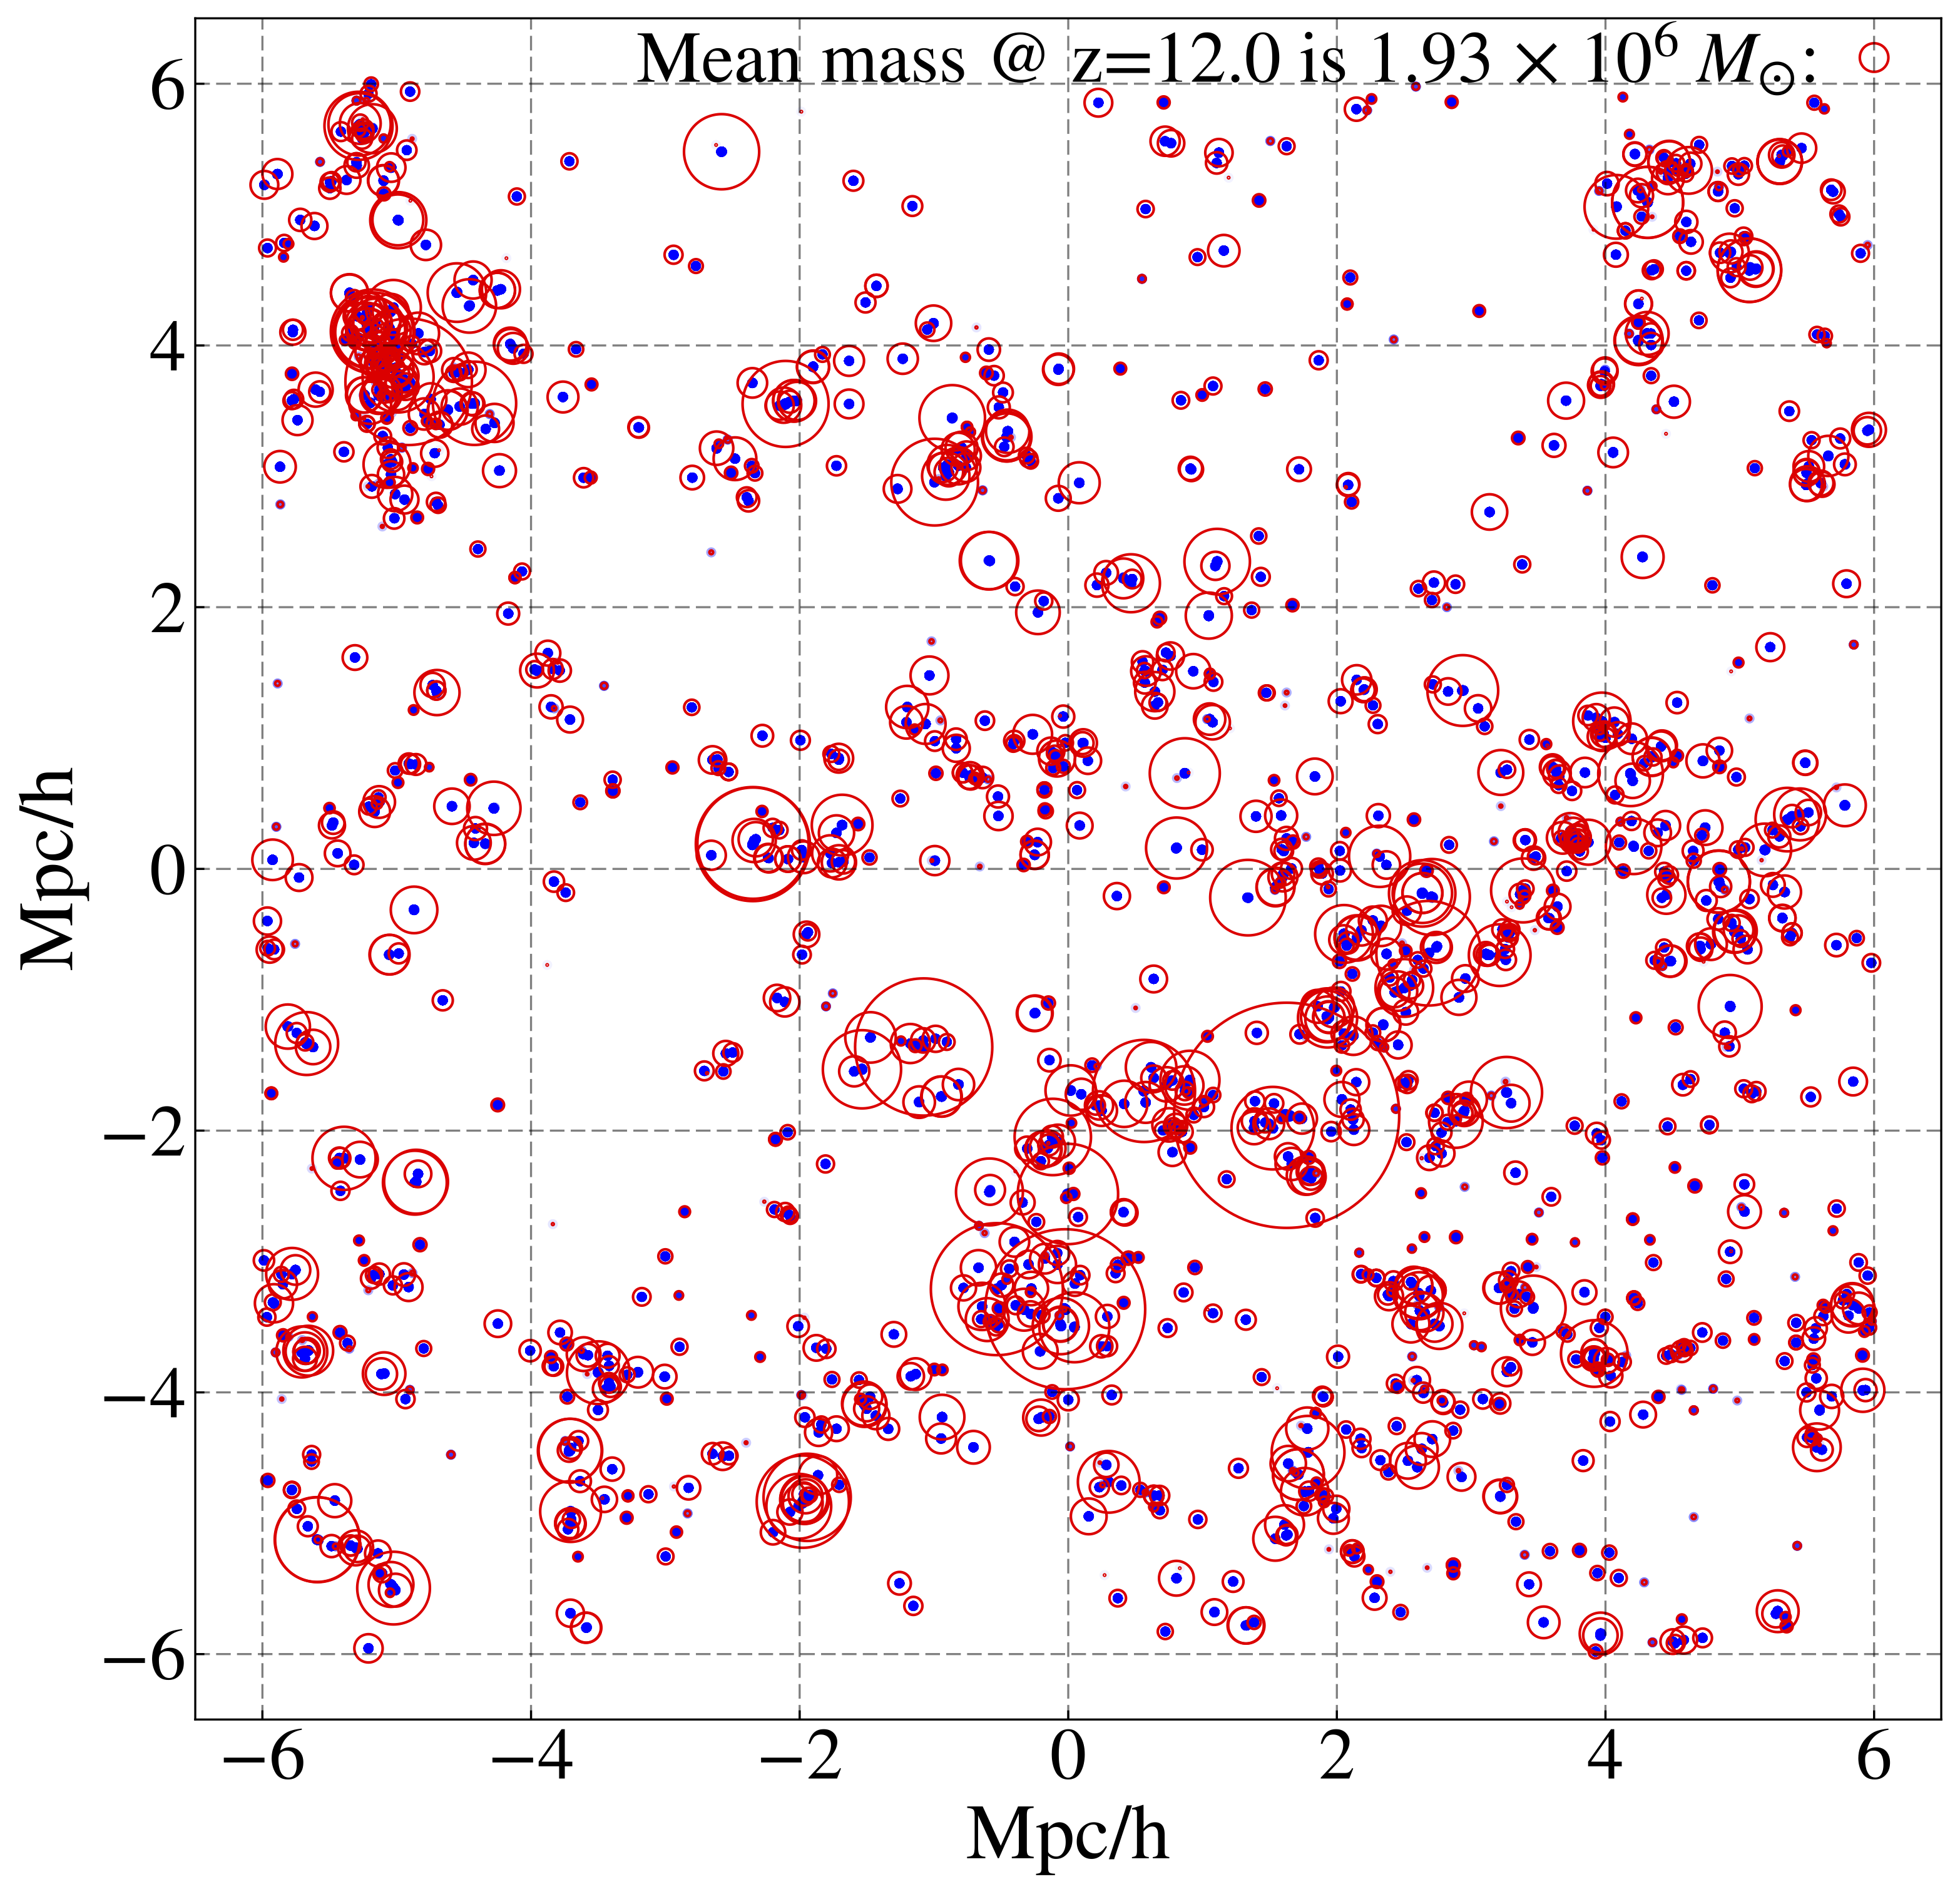
\includegraphics[width=1\columnwidth]{./AllHalos_120} \\
\end{tabular}
\caption{Stars particles (blue) and galaxies (red circles) in our simulation at redshifts 15 (left) and 12 (right). The size of the red circle corresponds to the stellar mass of the galaxy. The circle-size of an average stellar mass galaxy, for the redshift indicated, is indicated in the upper right corner. There are 314 galaxies at $z=15$ and 1388 at $z=12$. Scale is comoving Mpc/h.}
\label{fig:halos}
\end{center}
\end{figure*}

% virial radius.... maybe discuss in dissertation
%
%\begin{equation}\label{eq:vr}
%\begin{aligned}
%r_{\rm vir} = \left(\frac{3 M_{\rm DM}} {4 \pi \rho_{\rm crit}(z)\, \Omega_{\rm DM}(z)\, \Delta_{c}}\right)^{1/3} (1+z),
%\end{aligned}
%\end{equation}

%where $\Delta_{c} = 150$ is the average dark matter (DM) overdensity within $r_{\rm vir}$ and $M_{\rm DM}$ is the total mass of DM particles associated with the HOP halo. While a value of $200$ is typically used for determining the virial radius of galaxies, we found $\Delta_{c} = 150$ resulted in an $r_{\rm vir}$ that was more likely to include SPs associated with a single one of our high-redshift halos. We didn't use a fraction of the DM virial radius as is typically done when determining the radius of luminous material associated with a galaxy.

%%%%%%%%%%%%%%
\subsection{Galaxy Spectral Models}
The rest frame UV and filter-fluxes of our simulated galaxies are functions of the ages, metallicities, and masses of their constituent SP. We calculate our SP luminosities using a set of simple stellar population (SSP) spectral energy density (SED) models spanning the particles' ages and metallicity range. Our SEDs are based on \textit{STARBURST 99} \citep{2014ApJS..212...14L}, henceforth \textit{SB99} and \cite{2010A&A...523A..64R, 2003A&A...397..527S}, henceforth \textit{R10}. For all SPs with $Z_{\star} \geq Z_{\rm crit}$ our SEDs model a \cite{1955ApJ...121..161S} Initial Mass Function (IMF) normalized to $1\, M_{\odot}$. Since we have a precise age for each star particle, our SEDs model instantaneous bursts across the age range of SPs in the simulation. Pop III SP, with $Z_{\star} < Z_{\rm crit}$, are modeled using a log-normal IMF, again normalized to $1\, M_{\odot}$ and are based on the \textit{R10} SEDs for a zero metallicity population. The log-normal IMF is centered on a characteristic mass of $60M_{\odot}$ with $\sigma=1.0$ and a mass range $1\, M_{\odot} \le M \le 500\, M_{\odot} $. Conceptually, Pop III stars includes the mass of SPs with corrected metallicities $0 \le Z_{\star} < Z_{\rm crit}$ as well as the fractional mass of pristine stars, $P_{\star}\times M_{\star}$, with $Z=0$, that represent the mass-fraction of Pop III stars born in cells with incomplete mixing.  Since $P_{\star}$ captures the fraction of stellar mass with $Z_{\star} < Z_{\rm crit}$ the total mass of Pop III stars in each of our simulated galaxies is

\begin{equation}\label{eq:pop3mass}
\begin{aligned}
M_{\star, \rm III} = \sum_{n=1}^{N}{P_{\star, n} \; M_{\star, n}} ,
\end{aligned}
\end{equation}

% I have ensured that anytime the corrected metallicity, Z of a star particle is below Z_crit that the pristine fraction, P = 1.0

where $N$ is the total number of SPs in a galaxy and $M_{\star, n}$ is the mass of each SP. 

Our \textit{SB99} model SEDs were generated over an age range of 10 kyr to 1.12 Gyr, a little less than the age of the universe at $z=5$, in linearly-spaced steps of 0.5 Myr. Each SED covers the wavelength range $91 - 1.6\times10^{6} \AA$. We generated SEDs for metallicities of 0.02, 0.2, 0.4 and 1.0 $Z_{\odot}$, for each age, using the \textit{SB99}-implemented Padova \citep{2000A&AS..141..371G} models that include stellar and nebular emission through the onset of the thermal pulse AGB phase of stellar evolution. We supplemented the \textit{SB99} model with a set of \textit{R10} models for stars with $Z=5\times10^{-4}$ and $5\times10^{-6}\, Z_{\odot}$. This allows us to interpolate over the range $Z_{\rm crit} \le Z_{\star} \le Z_{\odot}$. The Pop III SEDs, by \textit{R10}, are based on $Z=0$ and cover the age range 10 kyr to 1 Gyr, in steps of 1 Myr. Again, the spectrum of all stars with $Z_{\star} < Z_{\rm crit}$ is modeled using this SED. Figure~\ref{fig:sed} depicts a sample of the rest-frame SEDs used in our analysis. The grey vertical dashed-lines in the plots indicate the rest-frame 1500 $\AA$ luminosity: our ultra-violet reference point for this study. We include the 5 Myr old Pop III SED in the plots for $Z > 0$ to illustrate how quickly the Pop III UV  luminosity falls-off with age. Stars with $Z > 0$ have more UV flux than Pop III stars of the same age after $\approx$ 3 Myr.
% Geneva may be better for young stars, but Padova models Z a factor of 2.5 lower than the Geneva models

\begin{figure*}[t]
\begin{center}
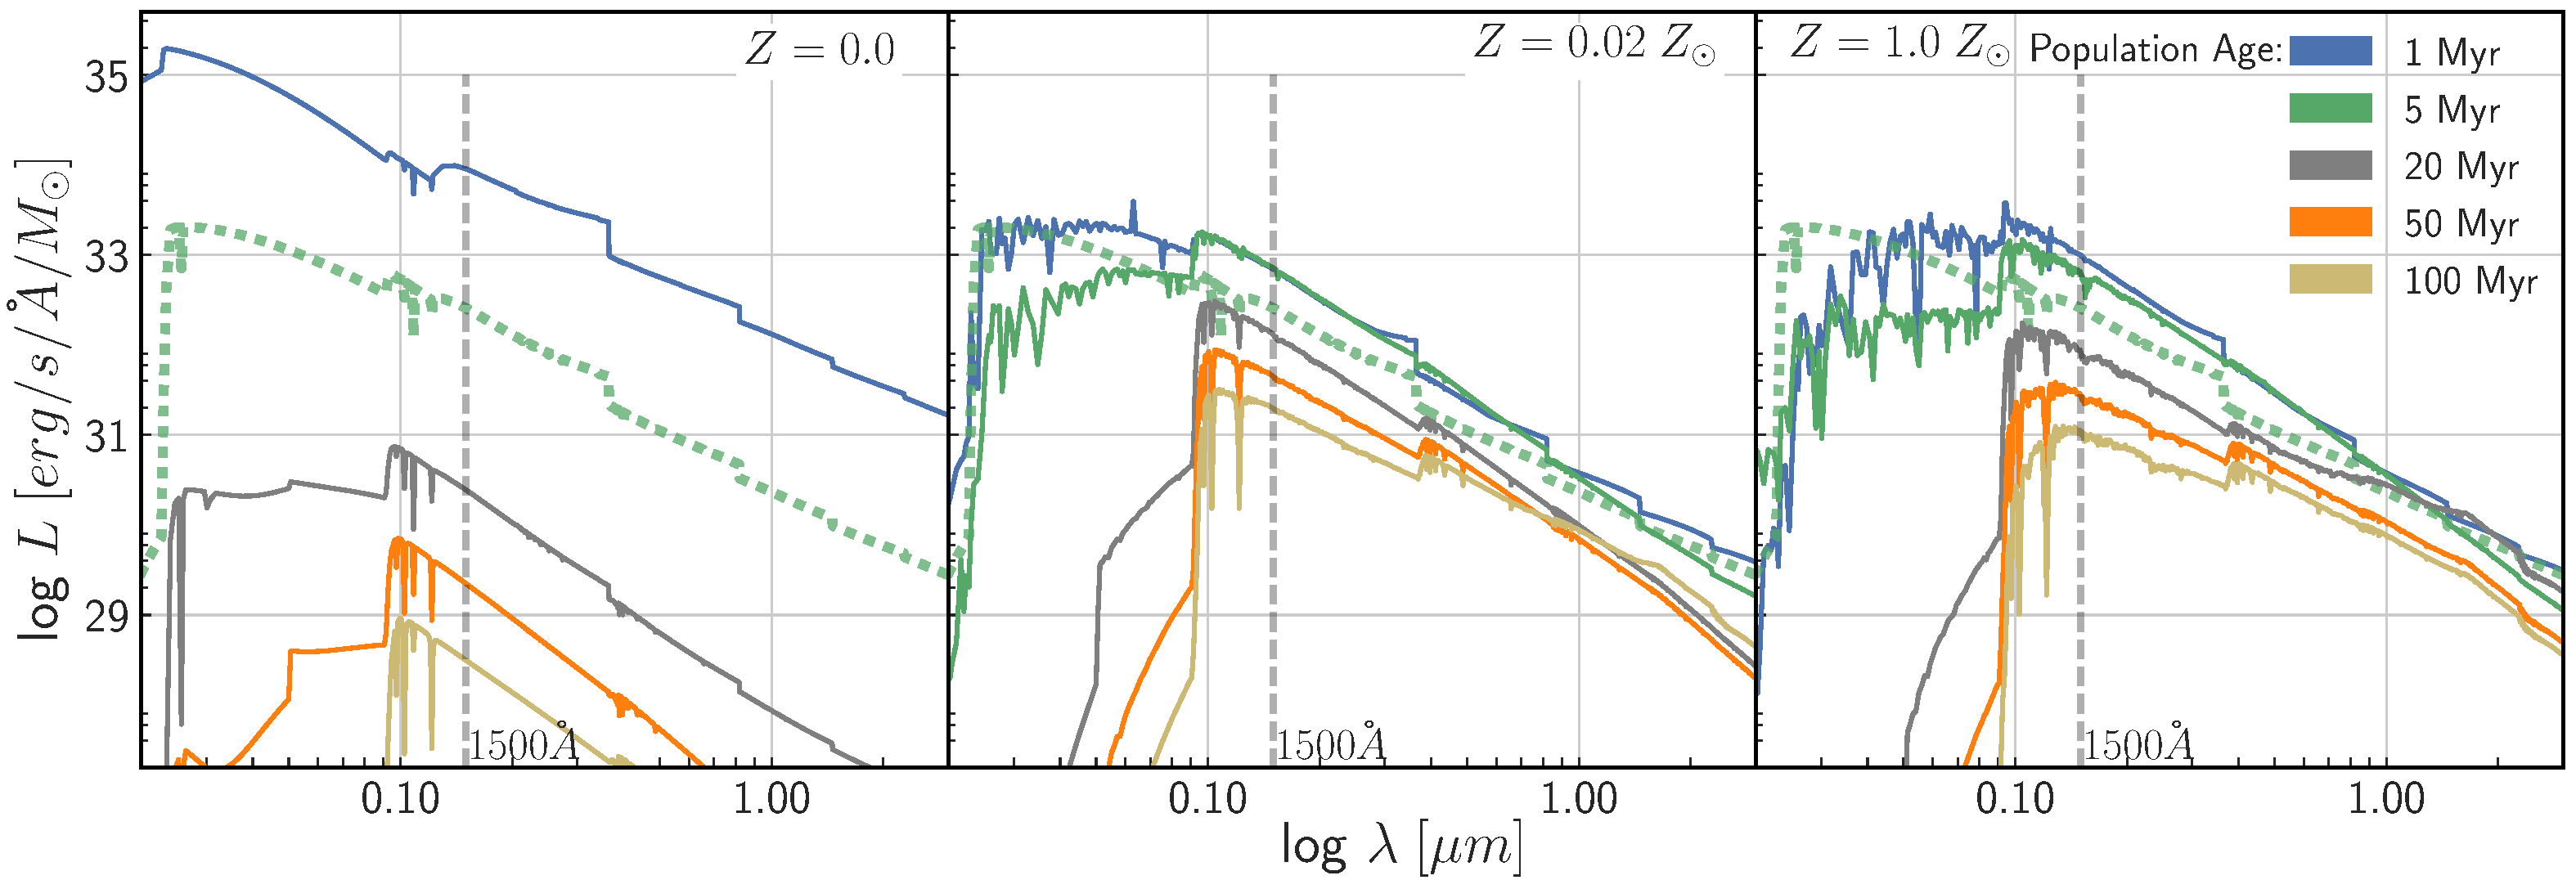
\includegraphics[width=2\columnwidth]{./SEDs}
\caption{Representative SEDs used to compute the filter and UV fluxes in our study. The grey dashed lines indicates the 1500 $\AA$ (our UV reference wavelength) luminosity for the models. The green-dashed line in the middle and right plots are the Pop III 5 Myr SED -- included for easy comparison. The  UV flux from young Pop III stars dominates for less than 5 Myr. In fact Pop III stars older than $\approx$ 3 Myr produce less UV flux than $Z>0$ populations with the same age.}
\label{fig:sed}
\end{center}
\end{figure*}

In order to compute the observational flux, we redshift each of our SEDs over the range $z=7$ to 16 applying Lyman forest and continuum absorption as described in~\cite{1995ApJ...441...18M}. 
%Figure~\ref{fig:lyAbs} depicts our implementation of this Lyman absorption model for a sampling of redshifts. 
This process, along with a spectral conversion from wavelength to frequency, transforms the rest frame \textit{SB99} and \textit{R10} SEDs ($erg/s/\AA/M_{\odot}$) into observational fluxes ($erg/s/Hz/cm^2/M_{\odot}$) across the range (in redshift, age and metallicity) of our SP. Equation~\ref{eq:LtoF} describes this conversion from rest-frame luminosity to observational flux for objects at cosmological distances:
\begin{equation}\label{eq:LtoF}
\begin{aligned}
S(\nu_{o},z)  = \frac{L_\nu(\nu_e)}{4 \pi D_L^2} (1+z), \\
f(\nu,z) =  S(\nu_{o}, z) \, \mathcal{M}(\nu_{o}, z),
\end{aligned}
\end{equation}
where the $\nu_{o}$ and $\nu_{e}$ are in Hz and refer to the observed and emitted reference frames, respectively, $D_L$ is the luminosity distance and $\mathcal{M}(\nu_{o}, z)$ is the~\cite{1995ApJ...441...18M} Lyman absorption function. We also generate the flux at a distance of 10pc to facilitate the generation of the absolute magnitude. This is done by setting $z=0$, $D_L = 10$ pc and $\mathcal{M}(\nu_{o}, z)=1.0$ in equation~\ref{eq:LtoF}.

% Explain how we got our magnitudes... 
We then convolve these bolometric fluxes with the set of JWST and Hubble filters listed in Table~\ref{tab:filters} (and depicted in Figure~\ref{fig:filts}). We also determine the rest-frame UV flux at 1500$\AA$. The observational fluxes are computed as follows:

\begin{equation}\label{eq:filterFlux}
\begin{aligned}
\mathcal{F}(R,z)=\frac{\int_{-\infty}^\infty{f(\nu,z) R(\nu)\, \frac{d\nu}{\nu} }}{\int_{-\infty}^\infty{R(\nu)\, \frac{d\nu}{\nu} }},
\end{aligned}
\end{equation}
where $f(\nu,z)$ is the flux of the star at redshift z, $R(\nu)$ is the filter response function and $\mathcal{F}(R,z)$ is the resulting bandpass flux. For the rest-frame UV flux, the filter response function is the simply the Dirac delta function shifted to the observational UV wavelength, $\nu_{\rm UV} =\nicefrac{c}{(1+z) 1500\AA}$, resulting in $R(\nu)= \delta(\nu - \nu_{\rm UV})$ which simplifies equation (\ref{eq:filterFlux}) to  

\begin{equation}\label{eq:uvFlux}
\begin{aligned}
\mathcal{F}(R,z)=f(\nu_{\rm UV},z) . 
\end{aligned}
\end{equation}
The result is a set of filter-flux tables that span the range of redshifts, ages, and metallicities for a normalized star of $1 M_{\odot}$ representing the Salpeter IMF, for $Z_{\star} \ge Z_{\rm crit}$, and the log-normal IMF for $Z_{\star} < Z_{\rm crit}$. This set of filter-flux tables, for each redshift, can be interpolated (in two dimensions) over the range of star particle ages and metallicities found in the simulation.

%\begin{figure}[h]
%\begin{center}
%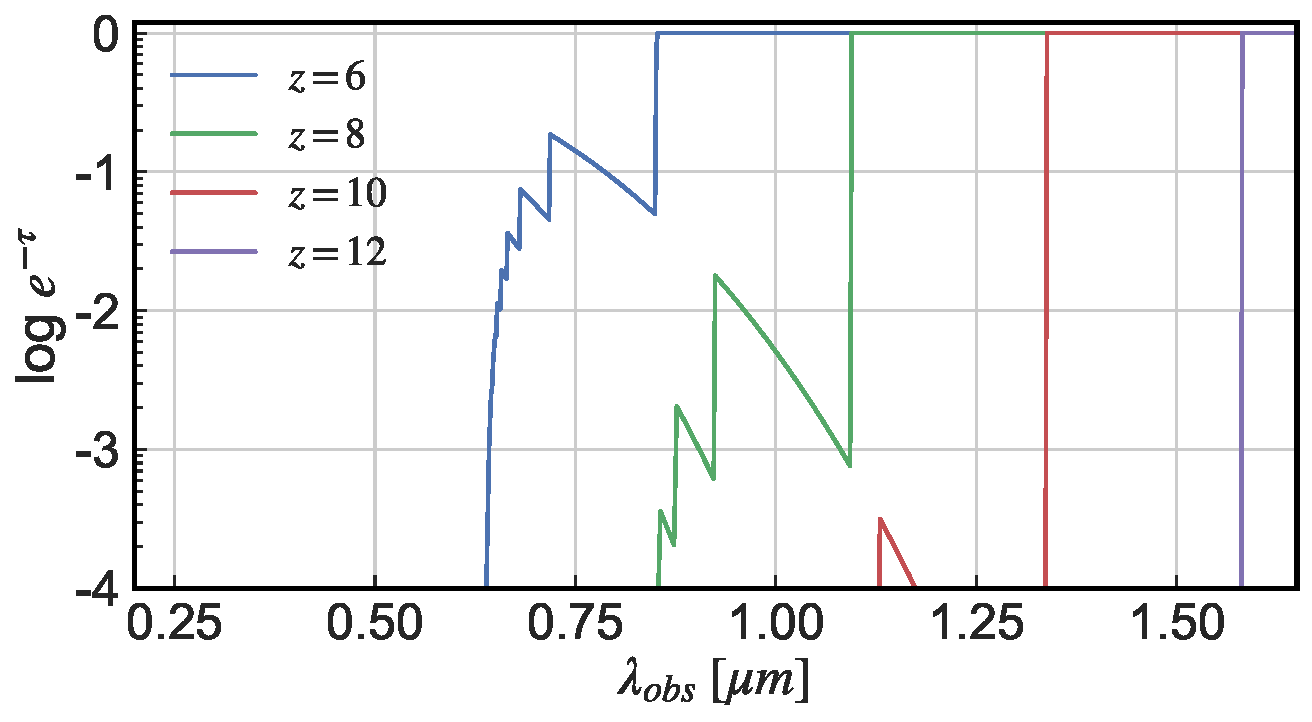
\includegraphics[width=1\columnwidth]{./lyAbs}
%\caption{Our Lyman absorption model expressed as a transmission function of observed wavelength. The model is based on the work of~\cite{1995ApJ...441...18M}. }
%\label{fig:lyAbs}
%\end{center}
%\end{figure}
%The reader will note that we have not discussed dust. Although there are a variety of methods used to estimate host-galaxy dust attenuation, there is a paucity of reliable, high-redshift models. Recent work based on the galaxy UV continuum slope, $\beta$, at $z>8$, is highly uncertain \citep{2016MNRAS.462..235L, 2016MNRAS.455..659W} but indicates attenuation on the order of $\langle A_{1600}\rangle < 0.5$ over the range of absolute magnitudes we report. We have not included this result in this work.

\begin{deluxetable}{c|l}
\tabletypesize{\footnotesize}
\tablecolumns{2} 
\tablecaption{Filters modeled in this study} 
\tablehead{System & Filter names } 
\startdata
JWST NIRCam & F150W,  F200W, F277W, F356W, F444W \\ \hline \\ [-1.5ex]
HST WFC3 & F125W, F160W  \\ \hline  \\ [-1.5ex]
Restframe UV & 1500 $\AA$
\enddata 
\label{tab:filters}
\tablenotetext{}{} % For extra space
\end{deluxetable} 

%%%%%%%%%%%%%%
\subsection{Simulated Observations}

We interpolate the filter and rest-frame UV fluxes linearly, in log-space, as a function of both star particle metallicity and age in order to compute the bandpass and rest-frame UV flux of our galaxies, at each redshift. 
%To streamline the computation, we first determine the set of unique star particle ages that are contained within each galaxy. Since star formation typically occurs in bursts, there are typically large numbers of stars with the same age. We next compute an interpolating function, in metallicity, for each of these ages and for each of the filters. 
The resulting fluxes are then scaled by the mass of each SP, accounting for $P_{\star}$, and summed to compute the total flux (in each filter) for the galaxy. We then transform the filter-fluxes into AB magnitudes via:
\begin{equation}\label{eq:obsmag}
\begin{aligned}
m_{\rm AB}(R,z) = -2.5\, log\,\big[\mathcal{F}(R,z) \big] - 48.60,
\end{aligned}
\end{equation}
where $\mathcal{F}(R,z)$ is the total flux from the galaxy as described above. Finally, we convert the observed magnitudes into absolute for our UV fluxes.

%%%%%%%%%%%%%%
\subsection{Simulation Setup}

We use \textsc{ramses} to evolve a 12 Mpc $h^{-1}$ on-a-side volume from mpgrafic \citep{2008ApJS..178..179P} generated initial conditions through $z=6.5$. The initial gas metallicity was $Z = 0,$ the initial $H_{\rm 2}$ fraction was $10^{-6},$ and we define $Z_{\rm crit} = 10^{-5} Z_\odot.$  The base resolution of $1024^{3}$ cells ($\textit{l}_{\rm min} = 10$) corresponding to a  grid resolution of 11.7 comoving kpc h$^{-1}$, and a dark matter particle mass of $1.79 \times 10^{6}\, M_{\odot}\, h^{-1}\, \Omega_{\rm \textsc{dm}}.$   We refined cells as they become $8\times$ over-dense, or when the local Jeans length is less than four times the current cell size, ensuring we always resolved the Jeans length with at least 4 cells. We allowed for up 8 additional refinement levels ($\textit{l}_{\rm max} = 18$), resulting in a average physical spatial resolution of 45.8 pc h$^{-1}$.  Our choice of parameters resulted in a range of star particle masses $3.7\times10^3\, M_{\odot} \leq M_{\star} \leq 6.3\times 10^4\, M_{\odot}$.  The highest refinement level reached was 15. The nonlinear length scale at the end of the simulation, z= 7,  was $47$ comoving kpc h$^{-1}$, corresponding to a mass of $4.6\times 10^{7}  M_\odot.$ 
We do not model sink particles (black holes - BH) in our simulation since BH feedback is not likely to be significant for our very early galaxies \citep{2008MNRAS.391..481S, 2004AAS...205.9421S}.  We tuned the code reionization parameters to ensure that the reionization redshift occurs at $z_{\rm reion} \approx 8.8$ as reported by the \cite{2015arXiv150201589P}. We do not model radiative transfer nor radiation pressure. While radiation pressure from massive young stars can be effective in disrupting star formation \citep{2012ApJ...745...50W, 2004ApJ...610...14W} it can also trigger it in dense clumps of gas \citep{2012A&A...546A..33T, 2010A&A...523A...6D}. While we have elected not to model its effects in this simulation it will be interesting to include its impacts in future studies. Finally, all magnitudes are in the AB system \citep{1983ApJ...266..713O}.

%%%%%%%%%%%%%%
%%%%%%%%%%%%%%
\section{Results}
In this section we present the characteristics of our simulated galaxies. We focus on the redshift range $8 \le z \le 16$ although some tables and figures may include data outside this range. Figure \ref{fig:sfrd} depicts the star formation rate density (SFRD) for our simulation along with an observationally-derived SFRD from \cite{2014ARA&A..52..415M} and the SFRD from our earlier, smaller (3 Mpc $h^{-1}$)$^3$ and higher resolution (23 pc $h^{-1}$) work \citep{2017ApJ...834...23S}. While our SFRD is higher than observations at $7 \le z \le 8$ it agrees well with the LF-based SFRD described by \cite{2016PASA...33...37F} (beige region to $z=10$). This SFRD is based on an integration of the reference luminosity functions in that work to $M_{\rm UV}$ = -13. Since the observationally-based SFRDs are likely under-sampled at $z>7$ \citep{2015ApJ...808..104O} it is more appropriate to compare our simulation to the LF-based SFRD.  

The figure also depicts the Pop III SFRD (green) as well as the `Classical Pop III' SRFD (red) that does not include the effects of subgrid mixing. We see that modeling turbulent subgrid mixing increases the SFRD for Pop III stars by an average factor of $\approx 2.1$ over the redshift range $7 \le z \le 16$. However, we also see that the earlier work produced a Pop III SFRD a full 2 times higher than this simulation at $z>9$. This points out the sensitivity of our results to our choice of modeling parameters such as simulation volume, resolution, star formation efficiency, star-formation density threshold, etc.  As such, we plan to carry out a parameter study to better characterize and bound the effects of modeling subgrid turbulent mixing on Pop III star formation. 

\begin{figure}[h]
\begin{center}
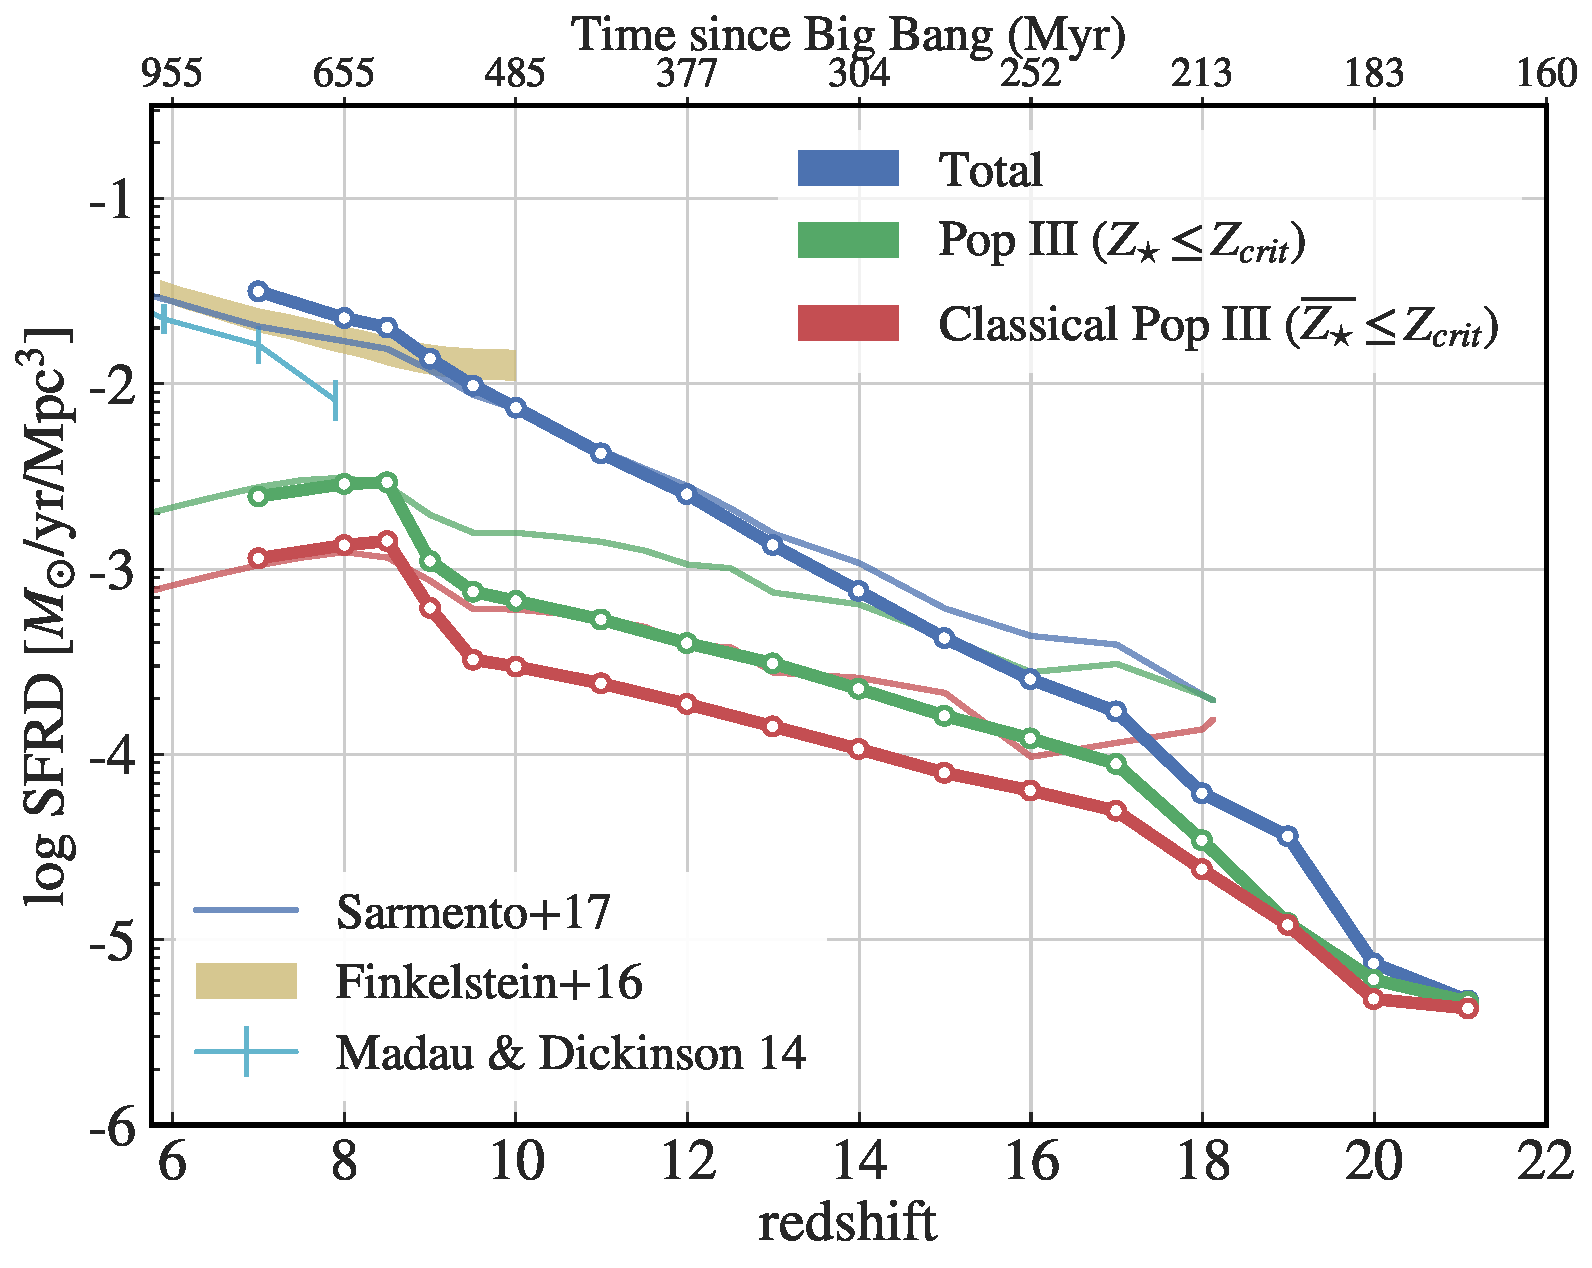
\includegraphics[width=1\columnwidth]{./SFRD_12}
\caption{Our SFRD along with observations by \cite{2014ARA&A..52..415M} and a LF-based SFRD by \cite{2016PASA...33...37F}. We have included the results from \cite{2017ApJ...834...23S} to depict the sensitivity of the Pop III SRFD to our choice of parameters. While our SFRD is above observations at $z\le 8$, it agrees well with an LF-based SFRD that incorporates galaxies down to $M_{\rm UV} = -13$}
\label{fig:sfrd}
\end{center}
\end{figure}

While the galaxy mass-metallicity relation at $z > 7$ is beyond current observational work \citep{2008A&A...488..463M}, Figure \ref{fig:gMZ} depicts this relationship for our simulated galaxies over the range $8 \le z \le 16$. The plots display the normalized probability per mass-bin, $\sum{\nicefrac{P(\overline{Z} / Z_{\odot})}{d(M_{\star}/M_{\odot})}} = 1.0$, for our galaxies. This normalization clearly depicts the expected mass-metallicity trend and also the mass range of Pop III galaxies (bottom row of bins in each plot) at each redshift. Each galaxies' average metallicity, $\overline{Z_{\rm G}}$, is computed using the corrected SP metallicities described in Equation (\ref{eq:zcorr}). Pop III galaxies, composed purely of SPs with $Z < Z_{\rm crit}$, have been grouped at $\overline{Z_{\rm G}}< 10^{-5} Z_{\odot}$.

\begin{figure*}[h!tp]
\begin{center}
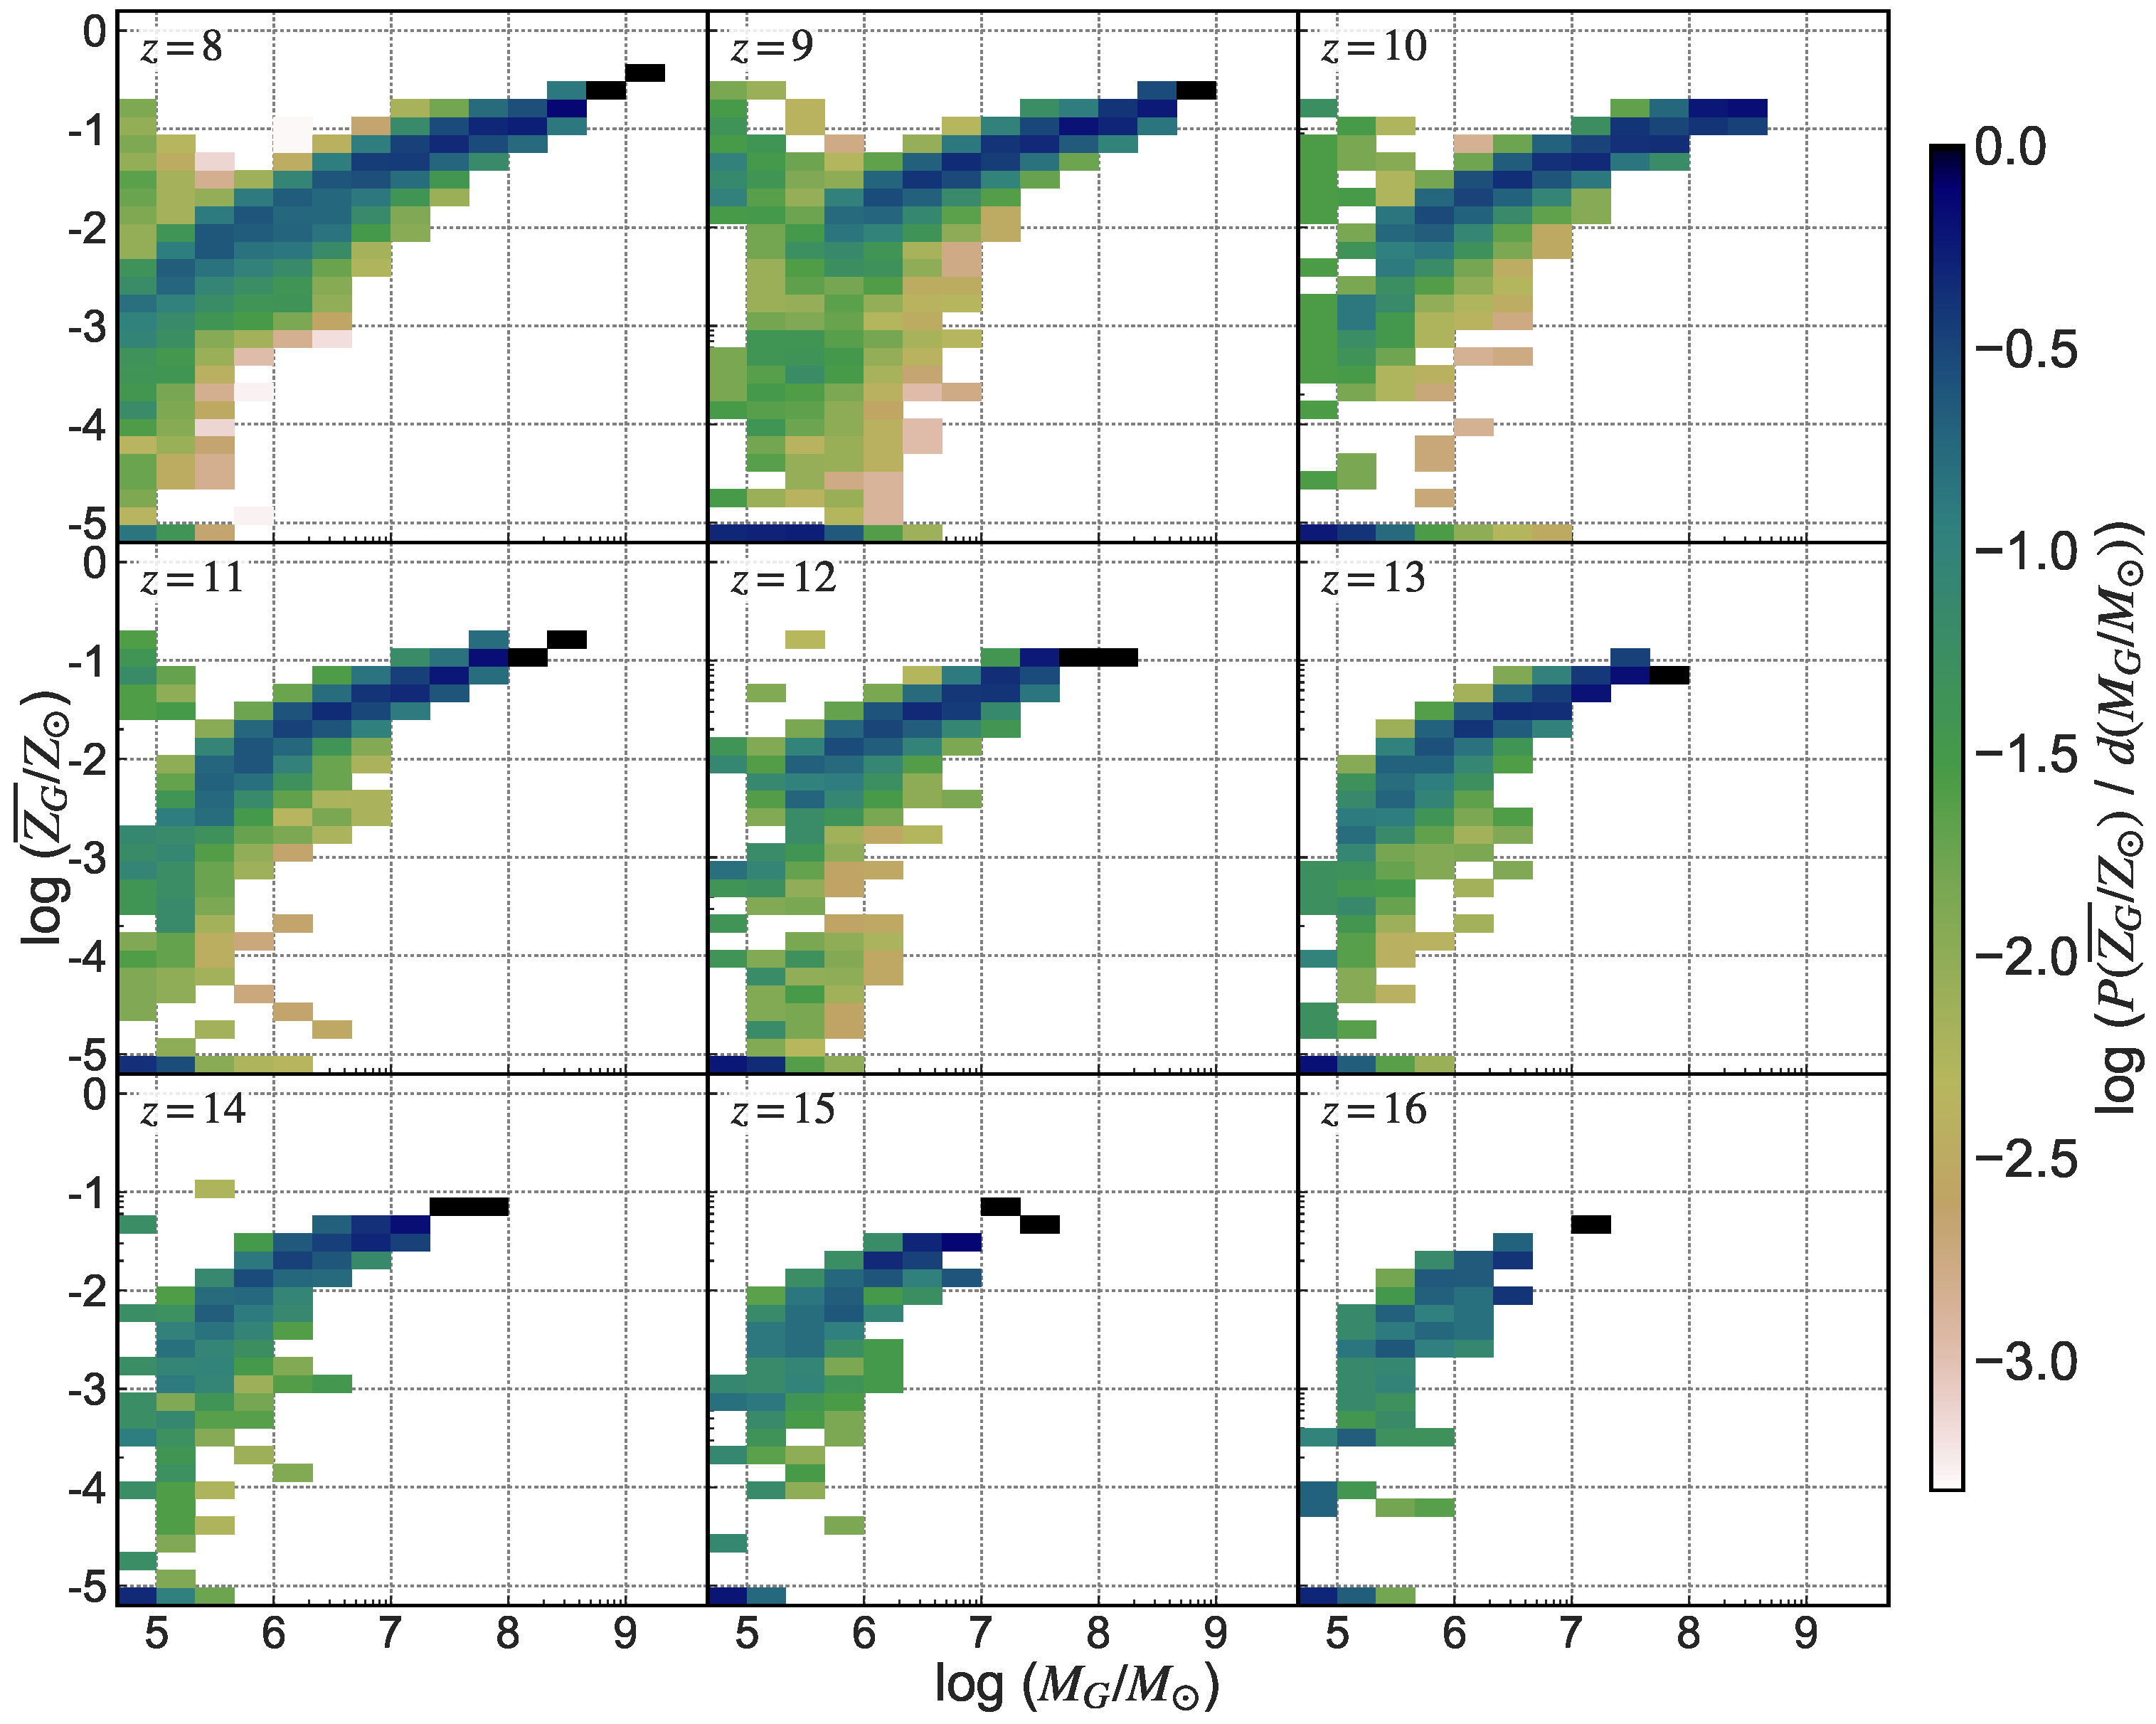
\includegraphics[width=2\columnwidth]{./Halo_Z_Histograms}
\caption{The probability, per mass bin, of finding a galaxy with a metallicity in the range $Z_{\odot} > Z \ge 9\times 10^{-6} Z_{\odot}$, where we have binned all Pop III galaxies at $Z < Z_{\rm crit} = 9\times 10^{-6} Z_{\odot}$. Purely Pop III galaxies with $M_{\star} > 10^{6} M_{\odot}$ are exceedingly rare within our simulation volume ($\approx$ 4800 Mpc$^3$, comoving).}
\label{fig:gMZ}
\end{center}
\end{figure*}

\begin{deluxetable*}{r|ccccccc} [h!t] 
\tablecaption{P($\nicefrac{f_{III}}{f_{Tot}} = 1$) per Mass bin} 
\tablehead{ & \multicolumn{7}{c} {$\overline{M_{\odot}}$ }\\
    z  &   $7.32\times 10^{4}$ &    $1.58\times 10^{5}$ &  $3.40\times 10^{5}$ &  $7.32\times 10^{5}$  &  $1.58\times 10^{6}$ &  $3.40\times 10^{6}$ &   $7.32\times 10^{6}$ }
\startdata
8 & 0.14$\pm{0.03}$ &  0.04$\pm{0.01}$ & $<0.01$ & 0.0 &  0.0 & 0.0 & 0.0 \\
9 &  0.48$\pm{0.08}$ & 0.51$\pm{0.06}$ & 0.55$\pm{0.05}$ & 0.23$\pm{0.02}$ & 0.02$\pm{0.01}$ & 0.01$\pm{0.01}$  & 0.0  \\
10 &  0.58$\pm{0.13}$ & 0.40$\pm{0.08}$ & 0.18$\pm{0.03}$ & 0.03$\pm{0.01}$ & 0.01$\pm{0.01}$ & 0.01$\pm{0.01}$ & $<0.01$  \\
11 & 0.43$\pm{0.07}$ & 0.28$\pm{0.05}$ & 0.01$\pm{0.01}$ & 0.01$\pm{0.01}$ & $<0.01$ & 0.0 & 0.0 \\
12 & 0.60$\pm{0.15}$ & 0.45$\pm{0.08}$ &  0.02$\pm{0.01}$ & $<0.01$ & 0.0 & 0.0 & 0.0 \\
13 &  0.65$\pm{0.18}$ & 0.21$\pm{0.05}$ & 0.02$\pm{0.01}$ & 0.01$\pm{0.01}$ & 0.0 & 0.0 & 0.0  \\
14 & 0.47$\pm{0.17}$ & 0.12$\pm{0.04}$ & 0.02$\pm{0.01}$ & 0.0 & 0.0 & 0.0 & 0.0  \\
15 & 0.62$\pm{0.22}$ & 0.18$\pm{0.06}$ & 0.0 & 0.0 & 0.0 & 0.0 & 0.0 \\
16 & 0.50$\pm{0.22}$ & 0.21$\pm{0.09}$ & 0.02$\pm{0.02}$ & 0.0 & 0.0 & 0.0 & 0.0 \\
\enddata  
\label{tab:MZR}
\tablecomments{The fraction of Pop III galaxies, in a specific mass-range, in our simulation. Errors are 1$\sigma$. Columns are labeled with the average mass for each bin. }
\end{deluxetable*}

Taken as whole we see that purely Pop III galaxies are not very massive and are comparable to the theoretical limit, $2.5\times10^{6}M_{\odot}$, discussed in \cite{2017MNRAS.467L..51Y}. In fact, over the entire redshift range the most massive Pop III galaxies occur at $z=10$ and have an average mass of $M_{\rm G} = 7.32 \times 10^{6}M_{\odot}$ -- where they make up less than 1\% of all galaxies with masses $M_{\rm G} > 4.64\times 10^{6}M_{\odot}$.  At lower redshift, $z=8$, Pop III galaxies span a smaller mass-range where the most massive, again less than 1\%,  have $M_{\rm G} \approx 3.4\times 10^{5}M_{\odot}$. Only a small fraction, 4\%, have an average mass $M_{\rm G} > 10^{5}M_{\odot}$ at this redshift. This is likely because the rate and location of Pop III star formation is changing. The Pop III SFRD turns over at $z=8.8$ and the Pop III fraction is no longer keeping pace with overall star formation. Since $z=8$ is post-reionization, the majority of new star formation is likely taking place within larger, shielded galaxies -- and within gas that has been polluted to levels above $Z_{\rm crit}$. However, moving out to $z=9$, we see more than 50\% of proto-galaxies in the two mass-bins between $10^{5} < M_{\rm G} \le 4.64\times10^{5}M_{\odot}$ are Pop III -- corresponding to a burst of star formation in pristine gas immediately before reionization. 

The low masses of purely Pop III proto-galaxies in the range $8\le z \le 11$, today's high-redshift frontier, partially explain the difficulty in finding Pop III galaxies. Table \ref{tab:MZR} depicts the Pop III fractions per mass-bin, as a function of galaxy redshift. However, as we shall discuss, a small percentage of young Pop III stars can contribute a significant fraction of a galaxy's flux. 

%%%%%%%%%%%%%%
\subsection{Luminosity functions}
Galaxy observations are characterized by their flux -- which in turn is determined by the galaxy's stellar populations. A small fraction of hot, young Pop III stars can contribute a large fraction of the galaxy's luminosity. Only the Pop III stars with $age < 3.5$ Myr contribute more flux than their polluted cousins, so detecting a galaxy dominated by Pop III flux means looking for a recent starburst such that a significant fraction of the flux from the entire galaxy is coming from these types of stars. We next look at the luminosity functions and Pop III flux-fractions derived from our simulation data. 

\begin{figure*}[h!tb]
\begin{center}
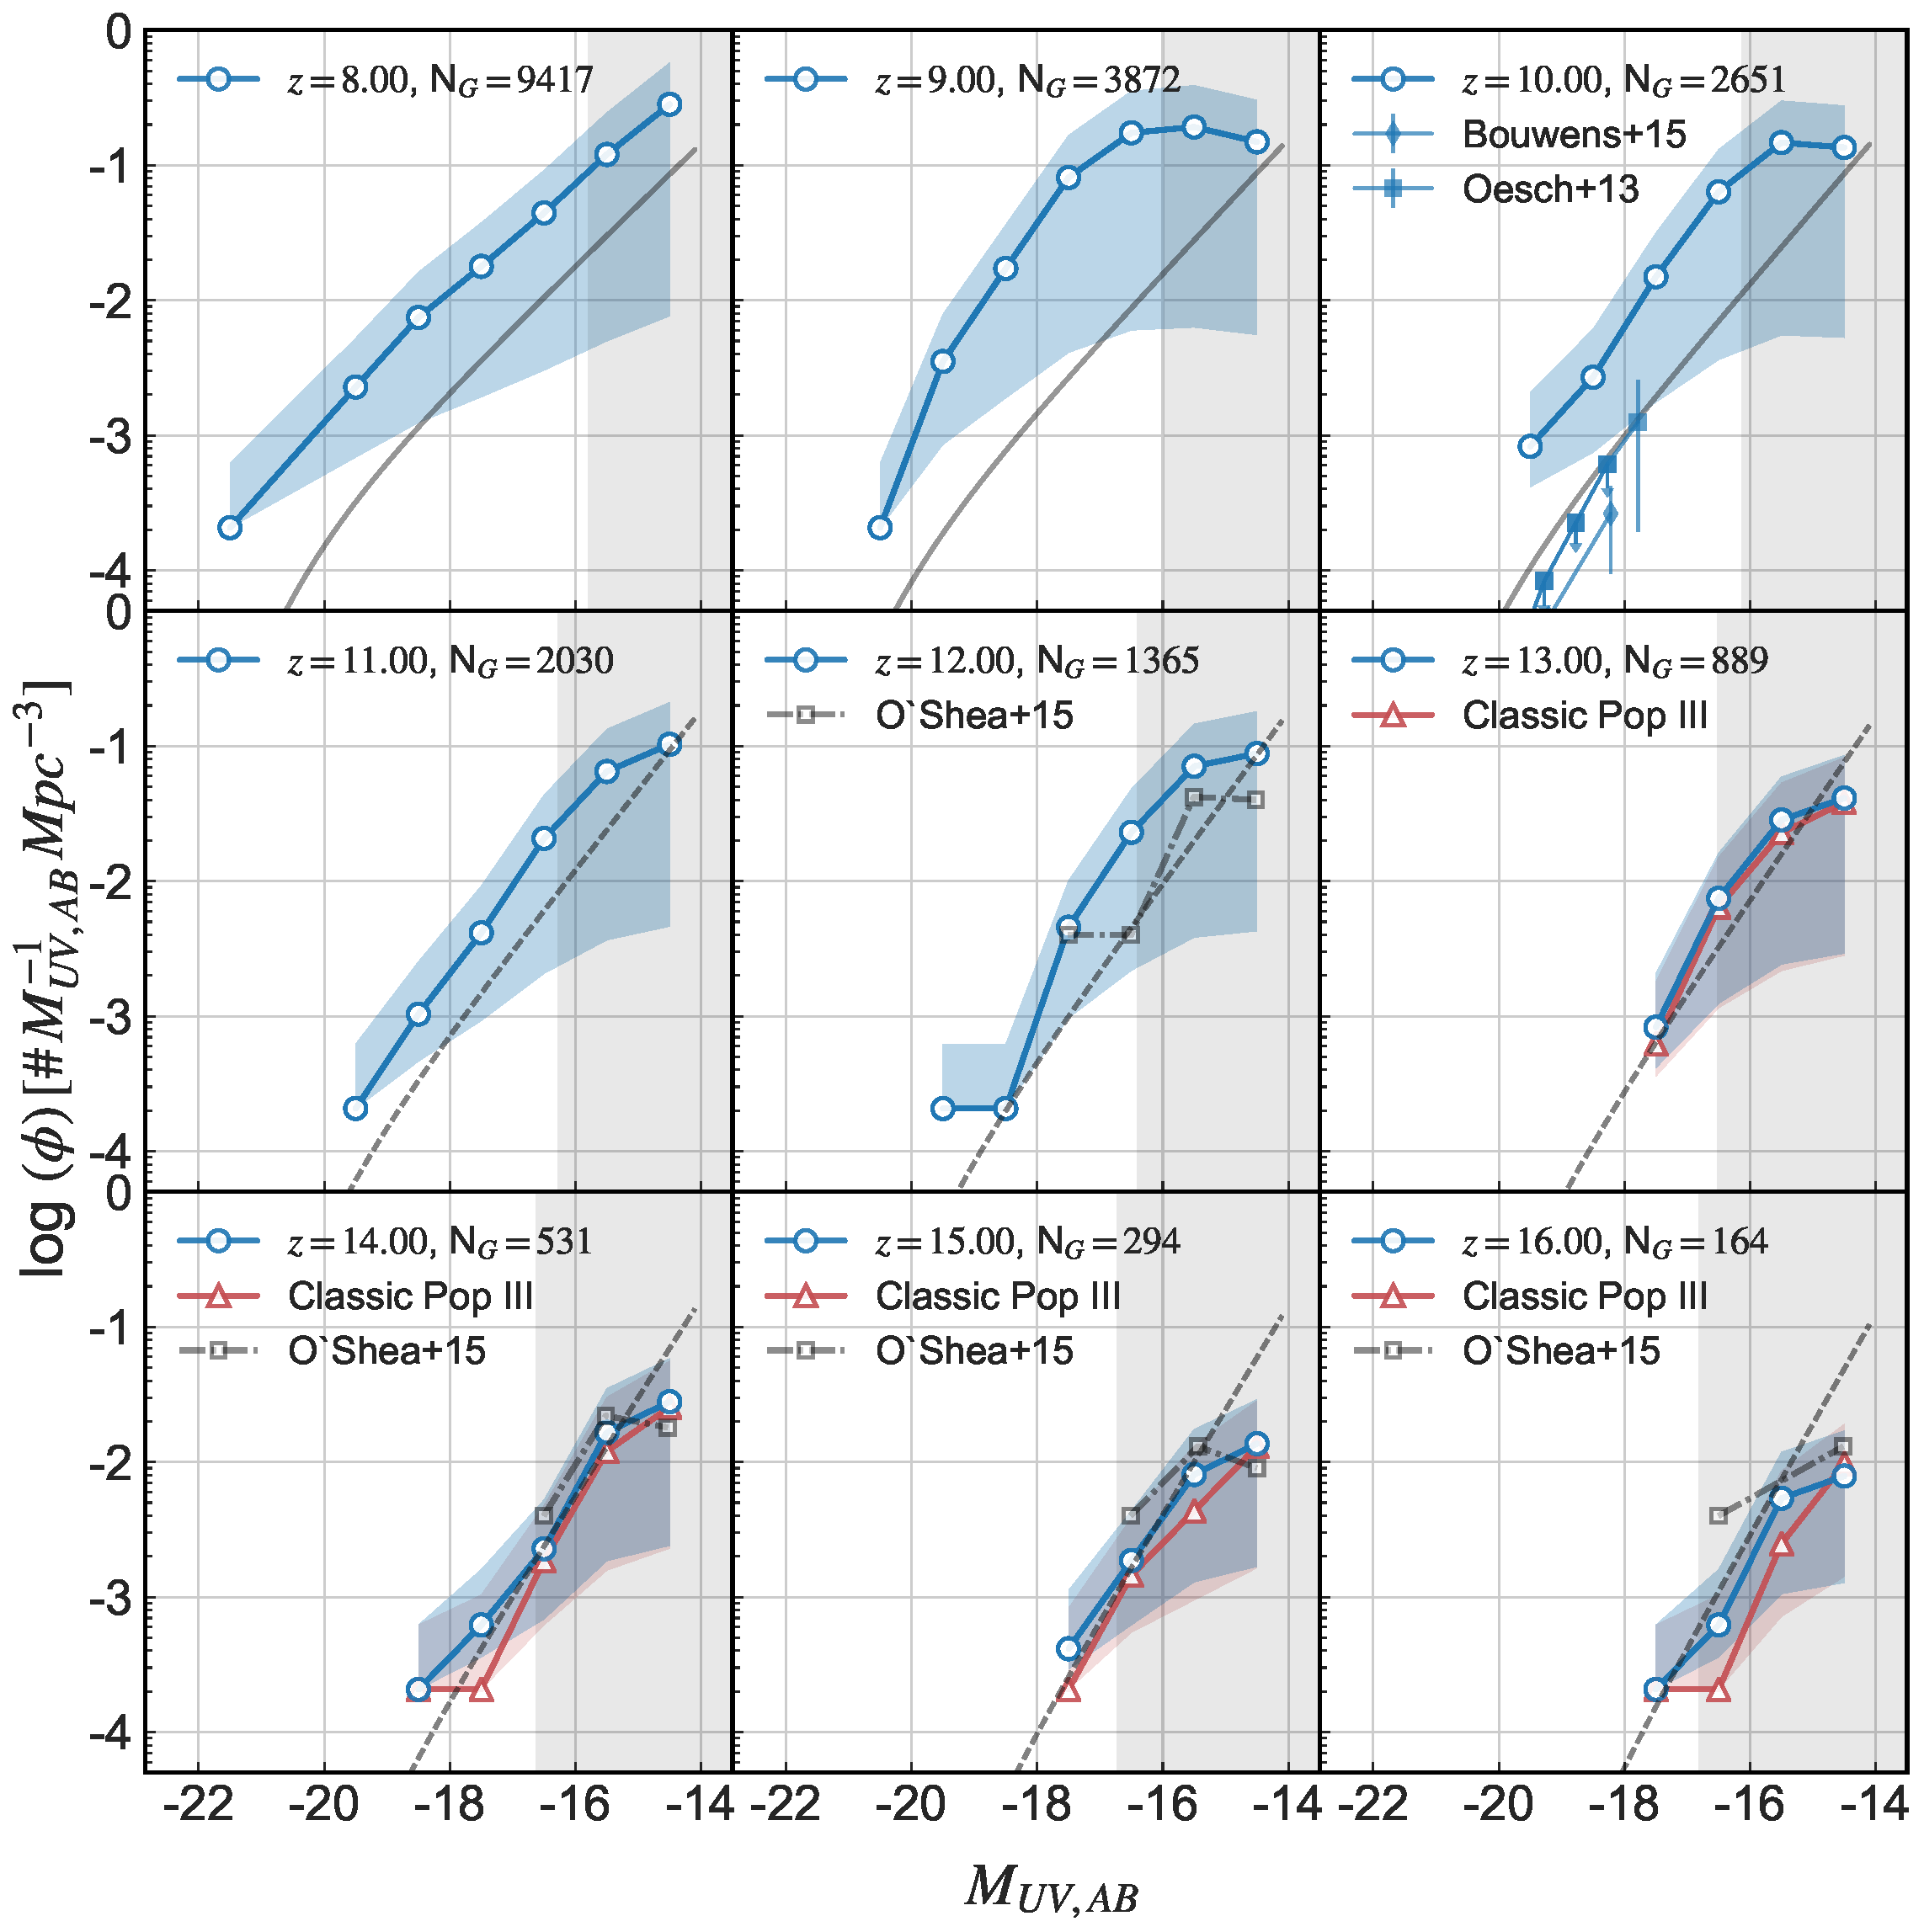
\includegraphics[width=2\columnwidth]{./haloUVMag_Summary_scatter9}
\caption{Luminosity functions, with 1$\sigma$ error bounds, derived from our simulation.  For $z\ge13$ the red lines model galaxies that include Pop III stars only in regions with $\overline{Z} < Z_{\rm crit}$. Dark grey lines are \cite{2016PASA...33...37F} Schechter fits. Dashed-grey lines are Schechter functions based on an extrapolation of the Schechter parameters also found in that work. For $z=10$, we have included \cite{2015ApJ...803...34B} and \cite{2013ApJ...773...75O} observational data, with error bars. For redshifts 12, 14, 15, and 16 we have included luminosity functions derived from the Renaissance Simulations by \cite{2015ApJ...807L..12O}. The shaded areas indicate the regions where $m_{\rm UV} > 31.4$ mag, a likely limiting magnitude for a JWST ultra-deep campaign. Our unusually bright LF for $z=9$ is due to the increase in the SFRD right before reionization at $z=8.8$.}
\label{fig:fit}
\end{center}
\end{figure*}

Given our total simulation volume of 4828 Mpc$^{3}$ we have data down to $\phi \approx 2\times10^{-4}\, \# \,M_{\rm UV}^{-1}\, Mpc^{-3}$.  Further, since star formation in our simulation is resolution-dependent we cannot track galaxy formation at scales below $\approx 260$ pc, physical. While such a small proto-galaxy is likely not detectable, even by JWST, it does prevent us from characterizing the inevitable turnover at the faint-end of the LF. Additionally, several such mini-halos may merge producing larger numbers of fainter galaxies than reported here. Given this context, Figure \ref{fig:fit} depicts the UV luminosity functions for all of our galaxies down to $M_{UV} = -14$ where the galaxy counts per magnitude bin begin to decrease due to the simulation's limited resolution. We have included both observational-derived and extrapolated \cite{1976ApJ...203..297S} functions by \cite{2016PASA...33...37F} for reference: Solid grey lines indicate Schechter functions derived from observations, while grey-dashed lines are an extrapolation of the Schechter parameters -- also from \cite{2016PASA...33...37F} -- to high-redshift. Schechter parameters for the observational data and extrapolations are listed in Table \ref{tab:schecParams}. We have also included observational data from \cite{2015ApJ...803...34B} and \cite{2013ApJ...773...75O} along with data from an analysis of galaxies in the Renaissance Simulations by \cite{2015ApJ...807L..12O}. Finally, for comparison, we include galaxy models in which Pop III stars form only in gas with $\overline{Z} < Z_{\rm crit}$ and $f_{\rm pol} < 1.0$ -- Classical Pop III stars -- for $z \ge 13$.  This is the era in which galaxy Pop III star fractions effect the LF.  These Classical Pop III LFs are denoted with red lines.

\begin{deluxetable}{r|ccc}[h!] 
\tablecaption{Schechter Function Parameters} 
\tablewidth{0.9\columnwidth} 
\tablehead{ z & log($\phi^{*}$) &  $\alpha$ &  $M^{*}_{\rm UV}$ }
\startdata
    8 & -3.75 & -2.13 & -20.52 \\
    9 & -3.94 & -2.24 & -20.39 \\
    10 & -4.13 & -2.35 & -20.25 \\ 
    11 & -4.29 & -2.47 & -20.11 \\ % Extrapolated from here
    12 & -4.49 & -2.58 & -19.98 \\
    13 & -4.69 & -2.69 & -19.84 \\
    14 & -4.89 & -2.81 & -19.71 \\
    15 & -5.08 & -2.92 & -19.57 \\
    16 & -5.28 & -2.03 & -19.44
\enddata  
\label{tab:schecParams}
\tablecomments{Schechter function parameters for the reference lines in the luminosity function plots. Data is from \cite{2016PASA...33...37F}. Values at $z > 10$ have been extrapolated based on a linear fit the parameters in that work.}
\end{deluxetable}


We note that all of our LFs at $z\le10$ lie above the faint-end of observationally-derived Schechter functions. However, it should be noted that data from our simulation begins at the faint-end where the observationally-derived models suffer from the greatest uncertainty. Assuming they are correct, our simulation produces either more galaxies per luminosity bin or brighter galaxies as compared to current models. While it is difficult to break this degeneracy given the information available, it is likely we are depicting brighter-than-average galaxies for several reasons. First, we do not account for dust. While attenuation likely has only a small effect on our high-redshift galaxies, at $M_{UV} < -19$ for $z \gtrsim 10$ \citep{2017arXiv170202146C}, if we extrapolate the work done by \cite{2015A&A...574A..19S} at $z\approx 6.8-7.5$ to $z=8-10$ we can account for $A_{UV}\approx 1.1\pm{0.2}$ of UV dust attenuation. This brings our data more in-line with the few observations at these redshifts.  Also, our simulation represents an average-density region of the universe and our LFs in the range $-18 < M_{UV} < -14$ compares favorably with the Renaissance Simulations' LFs at redshifts 12, 14, 15, and 16 -- the redshifts where average density luminosity functions are available from that work. 
%\begin{figure*}[h]
%\begin{center}
%\includegraphics[width=0.47\columnwidth]{./galaxyDensity_scatter}
%\caption{Galaxy density in this work and from the Renaissance Simulations. Our simulation produces more than a dex fewer galaxies per Mpc$^{3}$. The missing galaxies are due to the Renaissance Simulations` much higher resolution which allows it to track galaxy formation to smaller masses. These small galaxies do not influence the observable section of our luminosity functions.}
%\label{fig:galDens}
%\end{center}
%\end{figure*}

Our LF at $z=9$ is brighter than at $z=8$ over $-19 < M_{UV} \le -15$. Examining the SFRD, we see the Pop III star formation rate increasing sharply before $z\approx 9$ -- before reionization completes at $z=8.8$. In fact, looking back at Table \ref{tab:MZR} we see that immediately before reionization star formation begins to accelerate in mini-halos with $M_{\rm G} < 4.64\times 10^{5}\,M_{\odot}$ where the Pop III fraction of galaxies is 10$\times$ what it was at $z=10$. Also, the fraction of hot young stars, $age <$ 3.5 Myr, created at $z\approx 9$ is 12\% by mass and accounts for the excess brightness in the LF.  A short time later, 17 Myr, reionization completes and suppresses the subsequent star formation rate. By $z=8$ only 2\% of stars, by mass, are less than 3.5 Myr old. Such an effect, an acceleration of Pop III star formation then quenching by reionization, may have been at play in the real universe. Although we see this Pop III spike in our data, we do not feel confident pinpointing this epoch as a Pop III `era' because of our simulation's sensitivity to our chosen parameters. 

Our luminosity functions closely follow the predicted faint-end slope, $\alpha$, at $z>10$. Again, these Schechter curves (grey dashed lines) are based on a linear fit and extrapolation of the trends in $M*$, $\alpha$, and log $\phi *$ using observational data over the range $4\le z \le 8$.  Although we have no data at the bright-end of the LF, due to our small volume, we feel our LFs are representative of galaxy populations in the range plotted.

%%%%%%%%%%%%%%
\subsection{Pop III flux}

Since we are mainly concerned with the search for Pop III stars, we focus the remainder of our analysis on more detailed characteristics of our galaxies. Figure~\ref{fig:hist9} depicts the probability of finding a Pop III flux-fraction, as measured at $1500 \AA$, in the range $10^{-3} \le \nicefrac{f_{III}}{f_{Tot}} \le 1$ for our galaxies as a function of magnitude and redshift. When $\nicefrac{f_{III}}{f_{Tot}} < 10^{-3}$ we have mapped the value to $10^{-3}$. Note that probabilities are computed independently, as was done for the galaxy mass-metallicity relation, for each magnitude bin. 

The top-most row of bins in each plot represent a Pop III flux-fraction of at least 75\%: $P(\nicefrac{f_{III}}{f_{Tot}} \ge 0.75)$, while the next row down indicates a flux-fraction $P(0.75 > \nicefrac{f_{III}}{f_{Tot}} \ge 0.50)$.  Note that combining the probabilities in the 50\% and 75\% bins does not change the probabilities significantly from considering the 75\% bins alone.  Hence we use $75\%$ as our definition of ``significant Pop III flux'' and a ``Pop III-bright galaxy''.

Slightly more than 42\% of our galaxies at $z=9$ in the range $ -19 < M_{\rm UV} \le -17$ (corresponding to $m_{\rm UV}\approx 29.4$) have significant Pop III flux. This correlates with our observation of the increase in the SFRD at this epoch. At $z=11$, we find $P(\nicefrac{f_{III}}{f_{Tot}}\ge 0.75) \approx 40\%$ at $M_{\rm UV} \approx -18$. As we move to $z\ge14$ we note that most of these faint objects ($M_{\rm UV} \ge -17$)  are dominated by Pop III flux. This is the era of Pop III galaxies. These results are summarized in Table~\ref{tab:75PopIIFlux} where we have included the 1$\sigma$ errors based on the galaxy counts in each bin.  

\begin{deluxetable*}{r|cccccc} [h] 
\tablecaption{P($\nicefrac{f_{III}}{f_{Tot}} \ge 0.75$) per magnitude bin} 
\tablehead{ & \multicolumn{6}{c} {$M_{\rm UV}$ }\\
    z &   -19 &  -18 &  -17 &  -16 &  -15 &  -14 }
\startdata
  8.0 &  0.00 &  0.0 &  0.0 &  $0.05{\pm 0.02}$ &  $0.15\pm{0.02}$ &  $0.13{\pm 0.01}$ \\
  9.0 &  $0.28{\pm 0.12}$ &  $0.43{\pm 0.07}$ &  $0.44{\pm 0.03}$ & $0.27{\pm 0.02}$ & $0.05{\pm 0.01}$ &  $0.01{\pm 0.003}$ \\
 10.0 &  0.00 &  $0.23{\pm 0.13}$ &  $0.11{\pm 0.04}$ &  $0.15{\pm 0.02}$ &  $0.10{\pm 0.01}$ &  $0.06{\pm 0.01}$ \\
 11.0 &  0.00 &  $0.40{\pm 0.28}$ &  $0.10{\pm 0.07}$ &  $0.18{\pm 0.04}$ &  $0.23{\pm 0.03}$ &  $0.13{\pm 0.02}$ \\
 12.0 &  0.00 &  0.00 &  $0.27{\pm 0.11}$ &  $0.23{\pm 0.05}$ &  $0.21{\pm 0.03}$ &  $0.12{\pm 0.02}$ \\
 13.0 &  0.00 &  0.00 &  $0.25{\pm 0.25}$ &  $0.33{\pm 0.10}$ &  $0.39{\pm 0.05}$ &  $0.31{\pm 0.04}$ \\
 14.0 &  0.00 &  0.00 &  $0.67{\pm 0.33}$ &  $0.55{\pm 0.22}$ &  $0.49{\pm 0.08}$ &  $0.44{\pm 0.06}$ \\
 15.0 &  0.00 &  0.00 &  $0.50{\pm 0.50}$ &  $0.44{\pm 0.22}$ &  $0.67{\pm 0.13}$ &  $0.50{\pm 0.09}$ \\
 16.0 &  0.00 &  0.00 &  0.0 &  $0.67^{+ 0.33}_{- 0.47}$ &  $0.89^{+ 0.11}_{- 0.18}$ &  $0.50{\pm 0.12}$ \\
\enddata  
\label{tab:75PopIIFlux}
\tablecomments{The fraction of galaxies, per absolute magnitude bin, that have at least 75\% of their flux from Pop III stars. Errors, 1$\sigma$, are based on the number of galaxies in the each bin. Here we label the columns with the faint bin edge.}
\end{deluxetable*}

The results discussed so far include Pop III stars created in cells in which the turbulent mixing of metals was incomplete resulting in the enhanced Pop III SFRD we see in Figure~\ref{fig:sfrd}. The bottom row of Figure \ref{fig:hist9} depicts the Pop III flux-fraction for our galaxies when constraining Pop III star formation to cells with $\overline{Z} < Z_{\rm crit}$.  This is the no-mixing or Classical Pop III case. When considering only the Classical Pop III SPs we see that the enhancement of the Pop III SFRD due to our turbulent mixing model, an average of $\approx 2.1 \times$ the Classical rate, is responsible for a significant amount of flux at several redshifts. For instance, considering all `Classical galaxies' at $z=8$, only 1\% of the flux is from Pop III stars. However this increases to 5.6\% of the flux when we consider subgrid turbulent mixing: more than a 5$\times$ increase in flux. This result points to the importance of accurately modeling Pop III star formation since small changes in their density can significantly effect the predicted Pop III flux.  %Figure \ref{fig:p3enh} and Table~\ref{} capture these results.

\begin{figure*}[h!tb]
\begin{center}
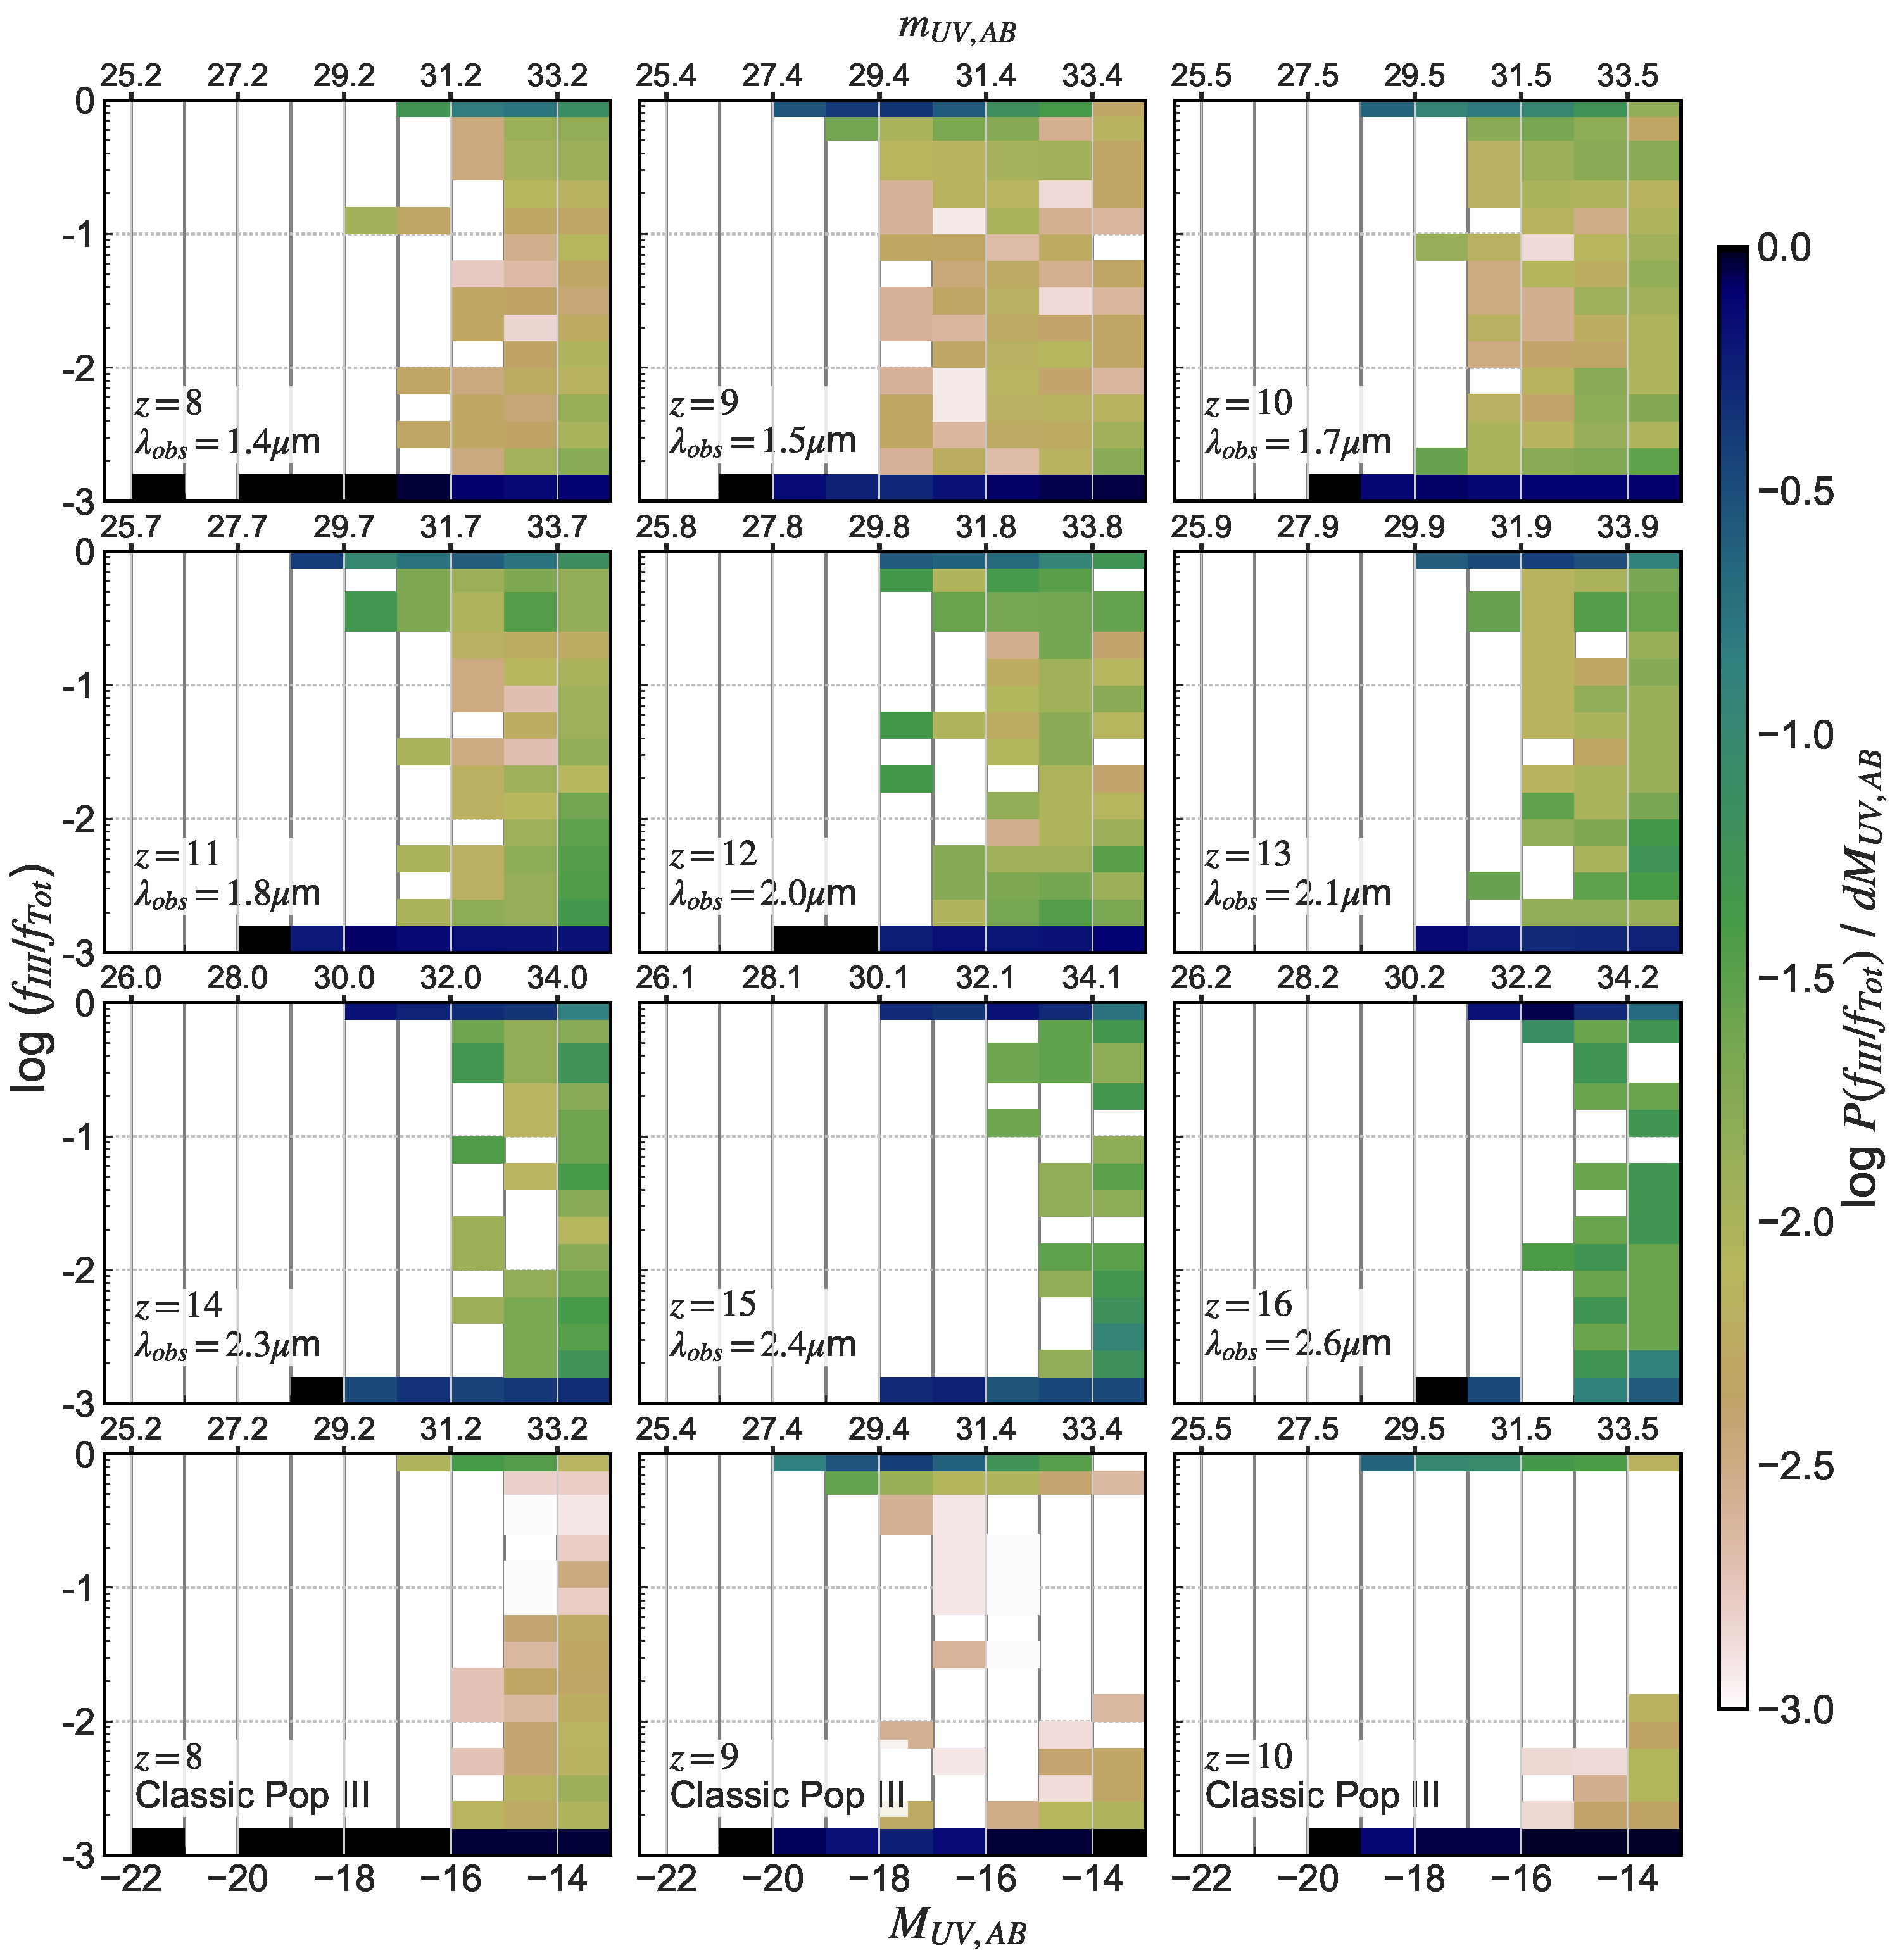
\includegraphics[width=2\columnwidth]{./PopIII_fraction-Histograms-all9}
\caption{The probability of finding a UV Pop III flux-fraction, $\nicefrac{f_{III}}{f_{Tot}}$, as a function of the redshift and magnitude of our galaxies.  When $\nicefrac{f_{III}}{f_{Tot}} < 10^{-3}$ we map the value to $10^{-3}$. Probabilities are computed independently for each magnitude bin. The top-most row of bins in each plot represent a Pop III flux-fraction of at least 75\%: $\nicefrac{f_{III}}{f_{Tot}} \ge 0.75$. The second row of bins represent $.75 > \nicefrac{f_{III}}{f_{Tot}} \ge 0.50$. At $z=11$, we find that 40\% of galaxies at $M_{\rm UV}  = 18$ have $\nicefrac{f_{III}}{f_{Tot}}> 75\%$.  The bottom row of plots depict the Pop III flux-fraction from our galaxies when only considering stars created in cells with $\overline{Z} < Z_{\rm crit}$.  Modeling turbulent subgrid mixing results in a Pop III SRFD that is a factor of 2 increase over the classical rate and these luminous stars contribute a significant fraction of the flux of these young galaxies. Axis labels along the top axis are observed UV magnitude, $m_{\rm UV}$.  We identify $\lambda_{obs}$ at each redshift: the wavelength of the 1500$\AA$ reference in the observational frame. }
\label{fig:hist9}
\end{center}
\end{figure*}

Next we consider the overall fraction of galaxies in the simulation that have a large fraction of Pop III flux. Table~\ref{tab:Pop3Gal} identifies the joint probability that a galaxy has at least a 75\% Pop III flux-fraction and $m_{UV} \le 31.4$ mag, which we take as the limiting magnitude for the un-lensed JWST ultra-deep campaign, as a fraction of all galaxies with $m_{UV} \le 31.4$ mag. We again see the bump in Pop III flux from our galaxies at $z=9$, immediately after a burst of Pop III star formation. At $z=10-11$ we note that between 15 and 18\% of our galaxies are Pop III-bright with an average mass-weighted metallicity between 1.11 -- 1.54 $\times10^{-3}\,Z_{\odot}$ indicating a large fraction of Pop II stars for these objects. At $z=12$, the fraction of Pop III-bright objects with $m_{\rm UV} \le 31.4$ mag increases to 30\% where they have an average stellar mass of $10^6\,M_{\odot}$. The mass-weighted average metallicity of these galaxies, $\overline{Z_{\rm G}} = 7.19\times10^{-4} Z_{\odot}$, is only slightly above our critical metallicity, $Z_{\rm crit} = 5\times10^{-4} Z_{\odot}$ indicating that the majority of stars in these objects are Pop III stars.  In fact, the average metallicity of the galaxies that meet our criteria are all well within a dex of our critical metallicity. Note that this does not necessarily imply a hard-UV flux since Pop III stars older than 3.5 Myr have spectra similar to their polluted brethren.   

\begin{deluxetable*}{lcccccc}[h!t]
\tablecaption{Pop III-bright galaxies detectable at $m_{\rm UV} \le 31.4$ mag} 
\tablehead{z &   $N_G/Mpc^{3}$ & $\overline{M}/M_{\odot}$ & $\overline{Z}/Z_{\odot}$ & P\tablenotemark{a} & $\overline{M_{UV}}$ & $\overline{m_{UV}}$ }
\startdata
   7.0 &         1.849 &            $1.00\times10^{6}$ &           $1.81\times10^{-3}$ &  0.018 &                       -16.2 &                        30.8 \\
  8.0 &         1.950 &            $5.31\times10^{5}$ &           $1.18\times10^{-3}$ &  0.047 &                       -16.2 &                        31.0 \\
  9.0 &         0.802 &            $7.81\times10^{5}$ &           $6.03\times10^{-4}$ &  0.327 &                       -17.0 &                        30.3 \\
 10.0 &         0.549 &            $1.08\times10^{6}$ &           $1.54\times10^{-3}$ &  0.147 &                       -16.7 &                        30.8 \\
 11.0 &         0.420 &            $1.31\times10^{6}$ &           $1.11\times10^{-3}$ &  0.177 &                       -16.9 &                        30.7 \\
 12.0 &         0.283 &            $1.02\times10^{6}$ &           $7.19\times10^{-4}$ &  0.296 &                       -16.9 &                        30.9 \\
 13.0 &         0.184 &            $1.23\times10^{6}$ &           $8.86\times10^{-4}$ &  0.412 &                       -17.0 &                        31.0 \\
 14.0 &         0.110 &            $1.78\times10^{6}$ &           $6.63\times10^{-4}$ &  0.500 &                       -17.3 &                        30.7 \\
 15.0 &         0.061 &            $1.54\times10^{6}$ &           $1.51\times10^{-3}$ &  0.200 &                       -17.2 &                        30.9 \\
 \enddata
\label{tab:Pop3Gal}
\tablenotetext{a}{The joint probability of finding a galaxy with $P(\nicefrac{f_{III}}{f_{Tot}} \ge 0.75\;and\;m_{UV} \le 31.4\, mag) / P(m_{UV} \le 31.4\, mag)$.}
\tablenotetext{}{We include the average mass, metallicity and magnitudes for the set of galaxies that meet our criteria. }
\end{deluxetable*}

We include Table \ref{tab:Pop3GalNM} which also identifies the fraction of observable Pop III-bright galaxies. However, these statistics only includes flux from Classical Pop III stars created in simulation cells with $\overline{Z} < Z_{\rm crit}$. As can be seen by comparing Tables \ref{tab:Pop3Gal} \& \ref{tab:Pop3GalNM}, the reduction in Pop III flux results in none of our galaxies meeting the criteria of at least a 75\% Pop III flux-fraction and $m_{UV} \le 31.4$ mag at $z>13$. At redshift 13 we see a decrease in fraction of Pop III-bright galaxies from 41\% to 17\%. The fraction of galaxies that are Pop III-bright across the redshift range $7 \le z \le 13$ is reduced an average of 7\%.

\begin{deluxetable*}{lcccccc}[h!t]
\tablecaption{Pop III-bright galaxies detectable at $m_{\rm UV} \le 31.4$ mag \\
 Classical Pop III stars only} 
\tablehead{z &   $N_G/Mpc^{3}$ & $\overline{M}/M_{\odot}$ & $\overline{Z}/Z_{\odot}$ & P\tablenotemark{a} & $\overline{M_{UV}}$ & $\overline{m_{UV}}$ }
\startdata
  7.0 &         1.849 &            $1.19\times10^{6}$ &           $1.75\times10^{-3}$ &  0.009 &                       -16.3 &                        31.0 \\
  8.0 &         1.950 &            $3.12\times10^{5}$ &           $4.63\times10^{-6}$ &  0.015 &                       -16.1 &                        31.1 \\
  9.0 &         0.802 &            $8.12\times10^{5}$ &           $5.97\times10^{-4}$ &  0.311 &                       -17.1 &                        30.4 \\
 10.0 &         0.549 &            $1.19\times10^{6}$ &           $1.20\times10^{-4}$ &  0.104 &                       -16.9 &                        30.7 \\
 11.0 &         0.420 &            $1.82\times10^{6}$ &           $8.74\times10^{-4}$ &  0.097 &                       -17.3 &                        30.4 \\
 12.0 &         0.283 &            $1.11\times10^{6}$ &           $6.62\times10^{-4}$ &  0.234 &                       -17.0 &                        31.0 \\
 13.0 &         0.184 &            $7.03\times10^{5}$ &           $1.61\times10^{-6}$ &  0.167 &                       -16.8 &                        31.1 \\
 14.0 &         0.110 &                        $0.00$ &                        $0.00$ &  0.000 &                         0.0 &                         0.0 \\
 15.0 &         0.061 &                        $0.00$ &                        $0.00$ &  0.000 &                         0.0 &                         0.0 \\
\enddata  
\label{tab:Pop3GalNM}
\tablecomments{Same as Table \ref{tab:Pop3Gal} but without considering the effects of subgrid mixing and its enhancement to the Pop III SFRD. The reduction in Pop III flux is apparent across our redshift range.}
\end{deluxetable*}

Figure \ref{fig:Zbright} depicts the distribution of our galaxies overlaid on the projected metallicity field of the simulation domain for $z=14 - 11$. In this figure, the location of Pop III-bright galaxies are indicated with cyan circles. If a Pop III-bright galaxy also has $m_{UV} \le 31.4$ mag we indicate it using a larger bright-cyan rectangle. Circle and rectangle size scale with the mass of stars in the galaxy. At redshift 14 there are only 3 Pop III-bright galaxies in our volume that have a magnitude $m_{UV} \le 31.4$ mag. This increases to 21 by $z=12$ but is down to 14 by $z=11$, a mere 48 million years later. This 30\% decline demonstrates the detectability dependence on the age of the stars in the galaxy: these objects shine brightly for fleetingly short periods of cosmic time. Most of the Pop III-bright galaxies form at the border of polluted areas or in regions of pristine gas away from larger halos. While our sample volume is relatively small, this result points out that Pop III-bright galaxies can be found both in relative isolation and near other, often larger galaxies with $Z_{\rm G} > Z_{\rm crit}$. Once again, modeling the mixing time required to pollute the gas above $Z_{\rm crit}$ is important here.

By examining fainter galaxies we can find a larger fractions of galaxies with significant Pop III flux at higher redshift. Table \ref{tab:Pop3Gal2} depicts characteristics of galaxies that have at least 75\% of their flux coming from Pop III stars while requiring that $m_{UV} \le 33$ mag, approximately the JWST 10x lensing limiting magnitude. With these criteria we now see that at $z=12$ the fraction of Pop III-bright galaxies is only 21\%, a result of more `regular' galaxies meeting the criteria $m_{UV} \le 33$ mag. At $z=14$ the fraction of Pop III-bright galaxies remains essentially unchanged. However, at $z=15$ the fraction of observable galaxies has jumped from 20\% to 64\% as a result of going to this faint magnitude and at $z=16$ more than 90\% of galaxies are Pop III-bright. If there are enough lensing opportunities JWST should detect a large fraction of Pop III-bright galaxies at $z=14$ and beyond.  

\begin{deluxetable*}{lcccccc}[h]
\tablecaption{Pop III galaxies detectable at $m_{\rm UV} \le 33$ mag} 
\tablehead{z &   $N_G/Mpc^{3}$ & $\overline{M}/M_{\odot}$ & $\overline{Z}/Z_{\odot}$ & P\tablenotemark{a} & $\overline{M_{UV}}$ & $\overline{m_{UV}}$ }
\startdata
7.0 &         1.849 &            $5.50\times10^{5}$ &           $2.27\times10^{-3}$ &  0.017 &                       -15.3 &                        31.7 \\
  8.0 &         1.892 &            $2.75\times10^{5}$ &           $2.19\times10^{-3}$ &  0.121 &                       -15.0 &                        32.2 \\
  9.0 &         0.784 &            $7.40\times10^{5}$ &           $8.08\times10^{-4}$ &  0.180 &                       -16.9 &                        30.5 \\
 10.0 &         0.549 &            $5.89\times10^{5}$ &           $2.28\times10^{-3}$ &  0.107 &                       -15.8 &                        31.7 \\
 11.0 &         0.402 &            $4.63\times10^{5}$ &           $1.83\times10^{-3}$ &  0.199 &                       -15.5 &                        32.1 \\
 12.0 &         0.283 &            $4.36\times10^{5}$ &           $1.12\times10^{-3}$ &  0.208 &                       -15.7 &                        32.1 \\
 13.0 &         0.184 &            $3.78\times10^{5}$ &           $1.10\times10^{-3}$ &  0.366 &                       -15.6 &                        32.3 \\
 14.0 &         0.110 &            $4.27\times10^{5}$ &           $8.36\times10^{-4}$ &  0.484 &                       -15.7 &                        32.4 \\
 15.0 &         0.061 &            $4.04\times10^{5}$ &           $8.30\times10^{-4}$ &  0.636 &                       -15.7 &                        32.5 \\
 16.0 &         0.034 &            $3.60\times10^{5}$ &           $6.87\times10^{-4}$ &  0.905 &                       -15.7 &                        32.5 \\
\enddata
\label{tab:Pop3Gal2}
\tablenotetext{a}{The joint probability of finding a galaxy with $P(\nicefrac{f_{III}}{f_{Tot}} \ge 0.75\;and\;m_{UV} \le 33\, mag) / P(m_{UV} \le 33\, mag)$.}
\tablenotetext{}{We include the average mass, metallicity and magnitudes for the set of galaxies that meet our criteria. }
\end{deluxetable*}

\begin{figure}[h!]
\begin{center}
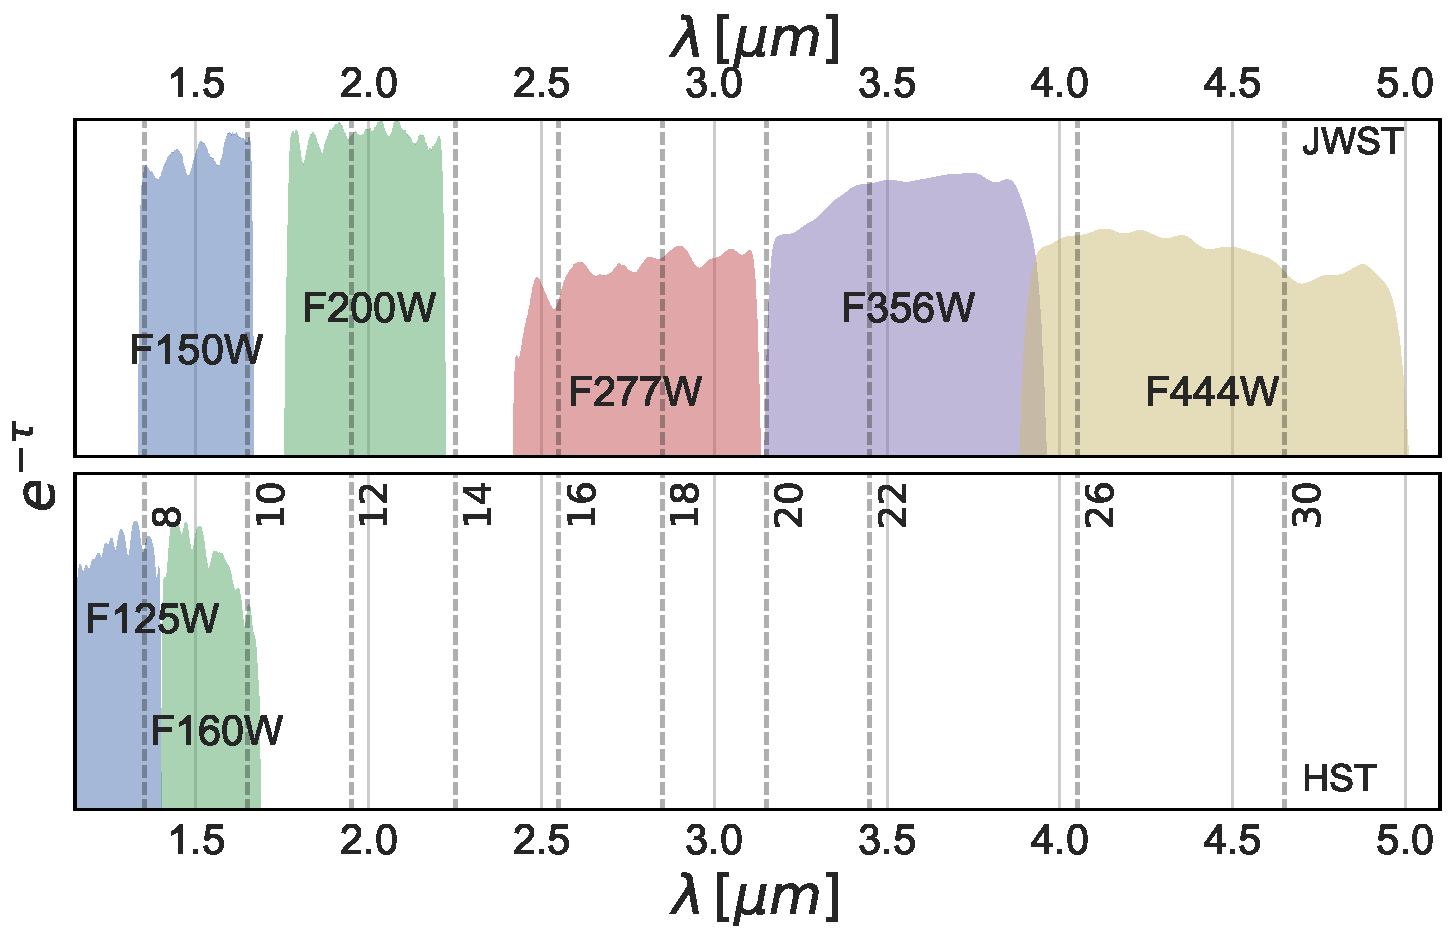
\includegraphics[width=0.95\columnwidth]{./allFilts.pdf} 
\caption{The JWST (top) and HST filters (bottom) included in our analysis. The vertical grey dashed lines indicate the rest-frame $1500\AA$ reference wavelength across a range of redshifts. These reference lines provide a quick orientation as to the portion of the galaxies' rest-frame spectrum that is sampled in each filter. For example, while a galaxy at $z=8$ is sampled (in the rest-frame) at $\approx 1500 \AA$ by F125W \& F150W, the F200W filter samples the same galaxy from $\approx 6000$ to $9000\AA$: i.e. -  $(11 - 8 + 1) * 1500 \AA $ to $(13 - 8 + 1) * 1500 \AA$.}
\label{fig:filts}
\end{center}
\end{figure}

\begin{figure*}[th!]
\begin{center}
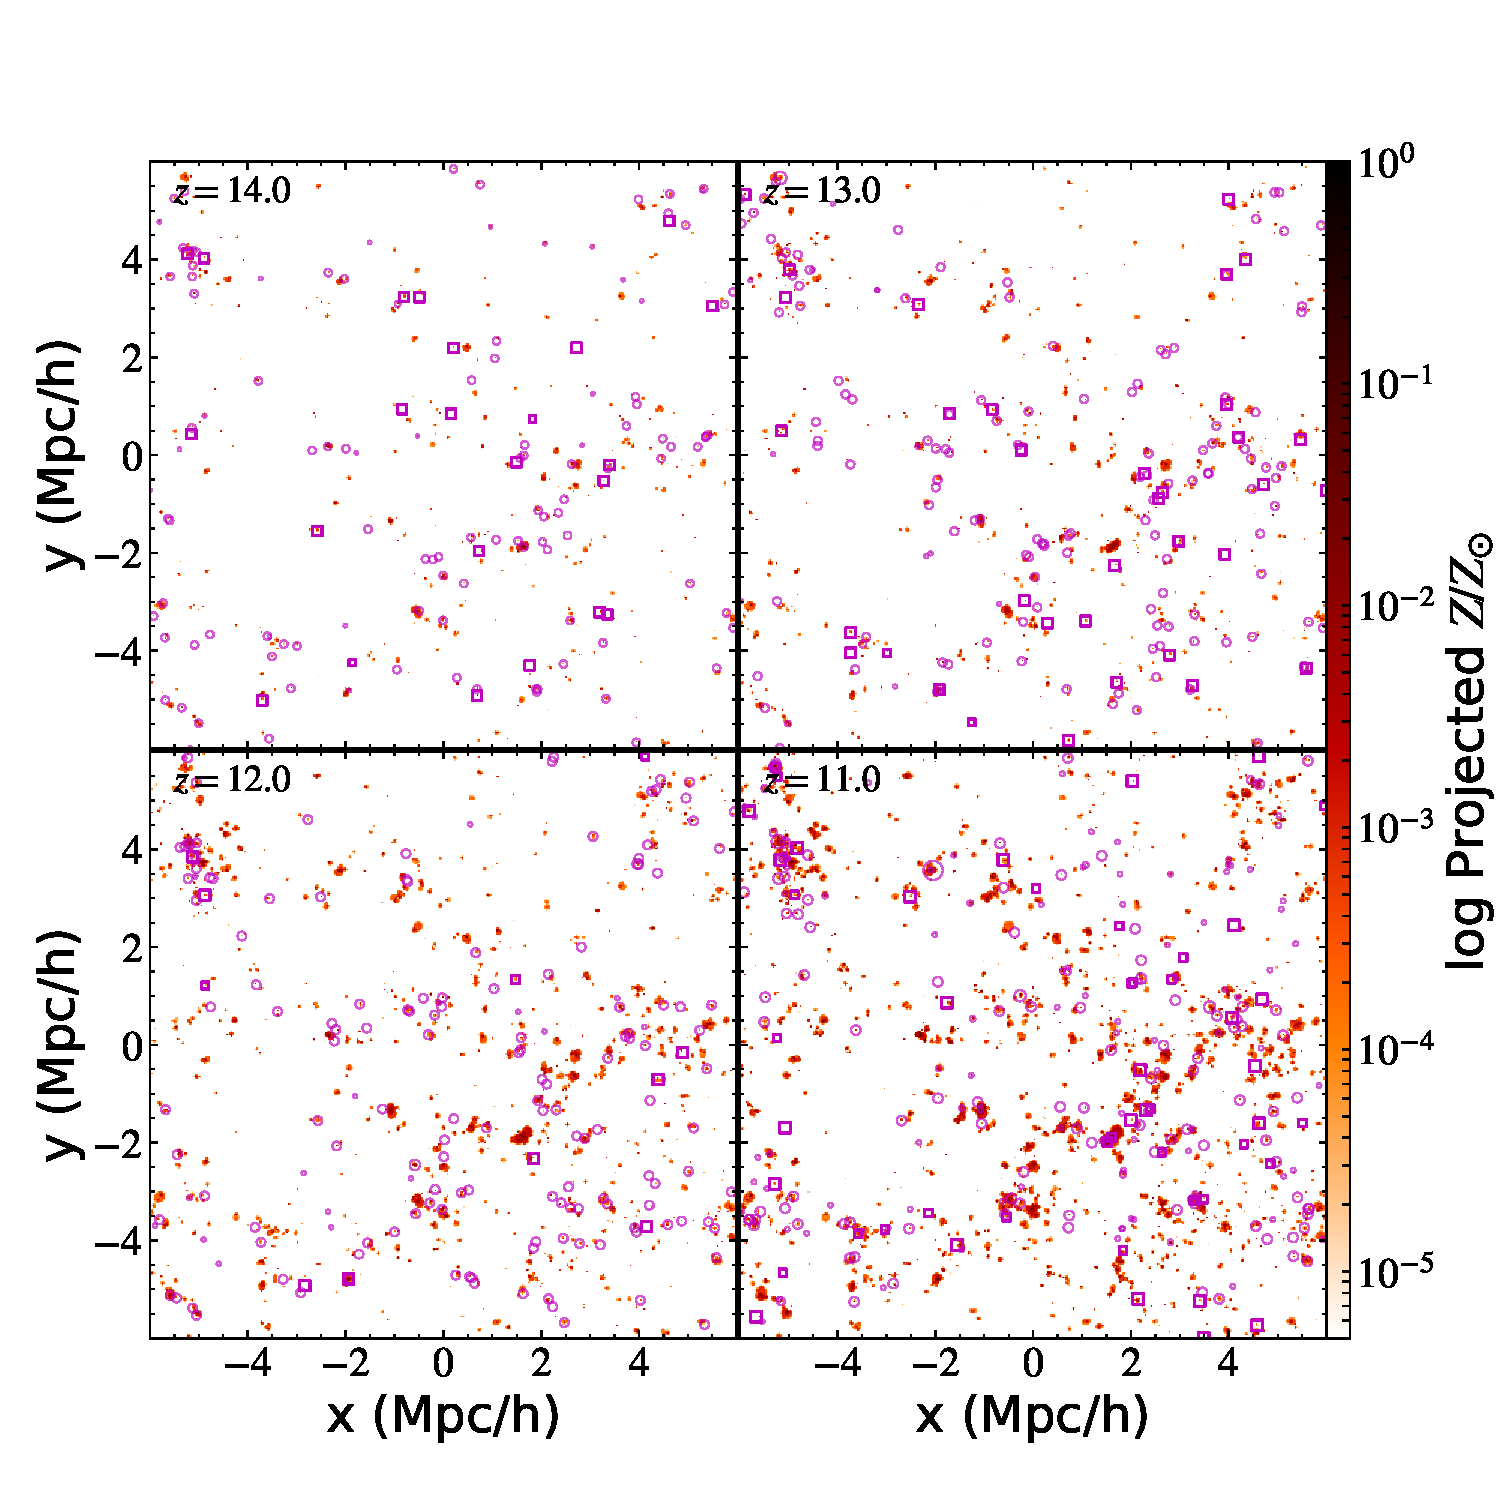
\includegraphics[width=2\columnwidth]{./Metallicity-bright-4}
\caption{These plots depict the projected, density-weighted, metallicity of the gas in the simulation box for $z=11-14$. Pop III-bright galaxies with $m_{UV} \le 31.4$ mag are indicated by cyan squares. Cyan circles are faint ($m_{UV} > 31.4$ mag) Pop III-bright galaxies.  The density-weighted projected metallicity of the gas is indicated by the colorbar. We note that the number of Pop III-bright galaxies in our simulation peaks at $z=12$ at 21 galaxies. This declines to 14 at redshift 11 exemplifying the short lifetime of Pop III hard-UV flux. While many of the Pop III-bright galaxies form on the edge of enriched material, or in relative isolation, there are several Pop III-bright galaxies that are associated with galaxies with $\overline{Z_{\rm G}} > Z_{\rm crit}$. The scale is comoving. }
\label{fig:Zbright}
\end{center}
\end{figure*}

\subsection{Filter fluxes}
In this section we discuss predictions for the space telescopes and filters described in Table \ref{tab:filters}. As with the rest-frame UV flux, we have not modeled dust for the results depicted in this section. Figure \ref{fig:filts} depicts the filter bandpasses we model along with observational references for the rest-frame UV wavelength across a range of redshifts. %These references allow the reader to quickly determine which filter corresponds to the UV LFs discussed earlier. 

The LFs derived from our simulated bandpasses are depicted in Figures \ref{fig:filtLF1} \& \ref{fig:filtLF2} and cover the redshift range $10 \le z \le 16$. If a particular filter or redshift is not included it is because there was no flux in the bandpass. For each of these plots we again indicate the JWST magnitude cutoff for the deep campaign, 31.4 mag, at the extrema of the redshift range depicted using a dark and light grey region, respectively. We note that, in general, galaxies with $M_{\rm UV} < -16$ are detected out to $z=12$ by filters redder than 1.2 $\mu$m and that galaxies at $z > 12$ typically require $M_{\rm UV} < -16.5$ and filters redder than 1.9 $\mu$m to be detected.

Starting with Figure \ref{fig:filtLF1}, the HST F125W filter was unable to detect any of our galaxies at $z > 10$. However, at $z=10$ our luminosity data for this filter agrees well, following the predicted faint-end slope, with an extrapolation of the few observations at this redshift \citep{2016ApJ...830...67B}. Using F160W we see our simulated galaxies are somewhat bright at $z=10$, but within $1\sigma$ of the model, while our $z=12$ data are lower than predictions. This agreement with Schechter functions based on Hubble deep-field surveys is evidence that our simulation is producing reasonable results out to this redshift. There was no guarantee that our enhanced Pop III modeling would produce galaxy fluxes that agree with observations.

The situation is similar for the JWST bandpass filter at 1.5 $\mu$m (F150W) -- our data brackets the extrapolated Schechter range.  This wide-band filter straddles the Lyman-$\alpha$ line in the rest frame so we are seeing the attenuation of UV photons by the intergalactic medium (IGM) as we go from $z=10 \rightarrow 12$.

\begin{figure*}[h]
\begin{center}
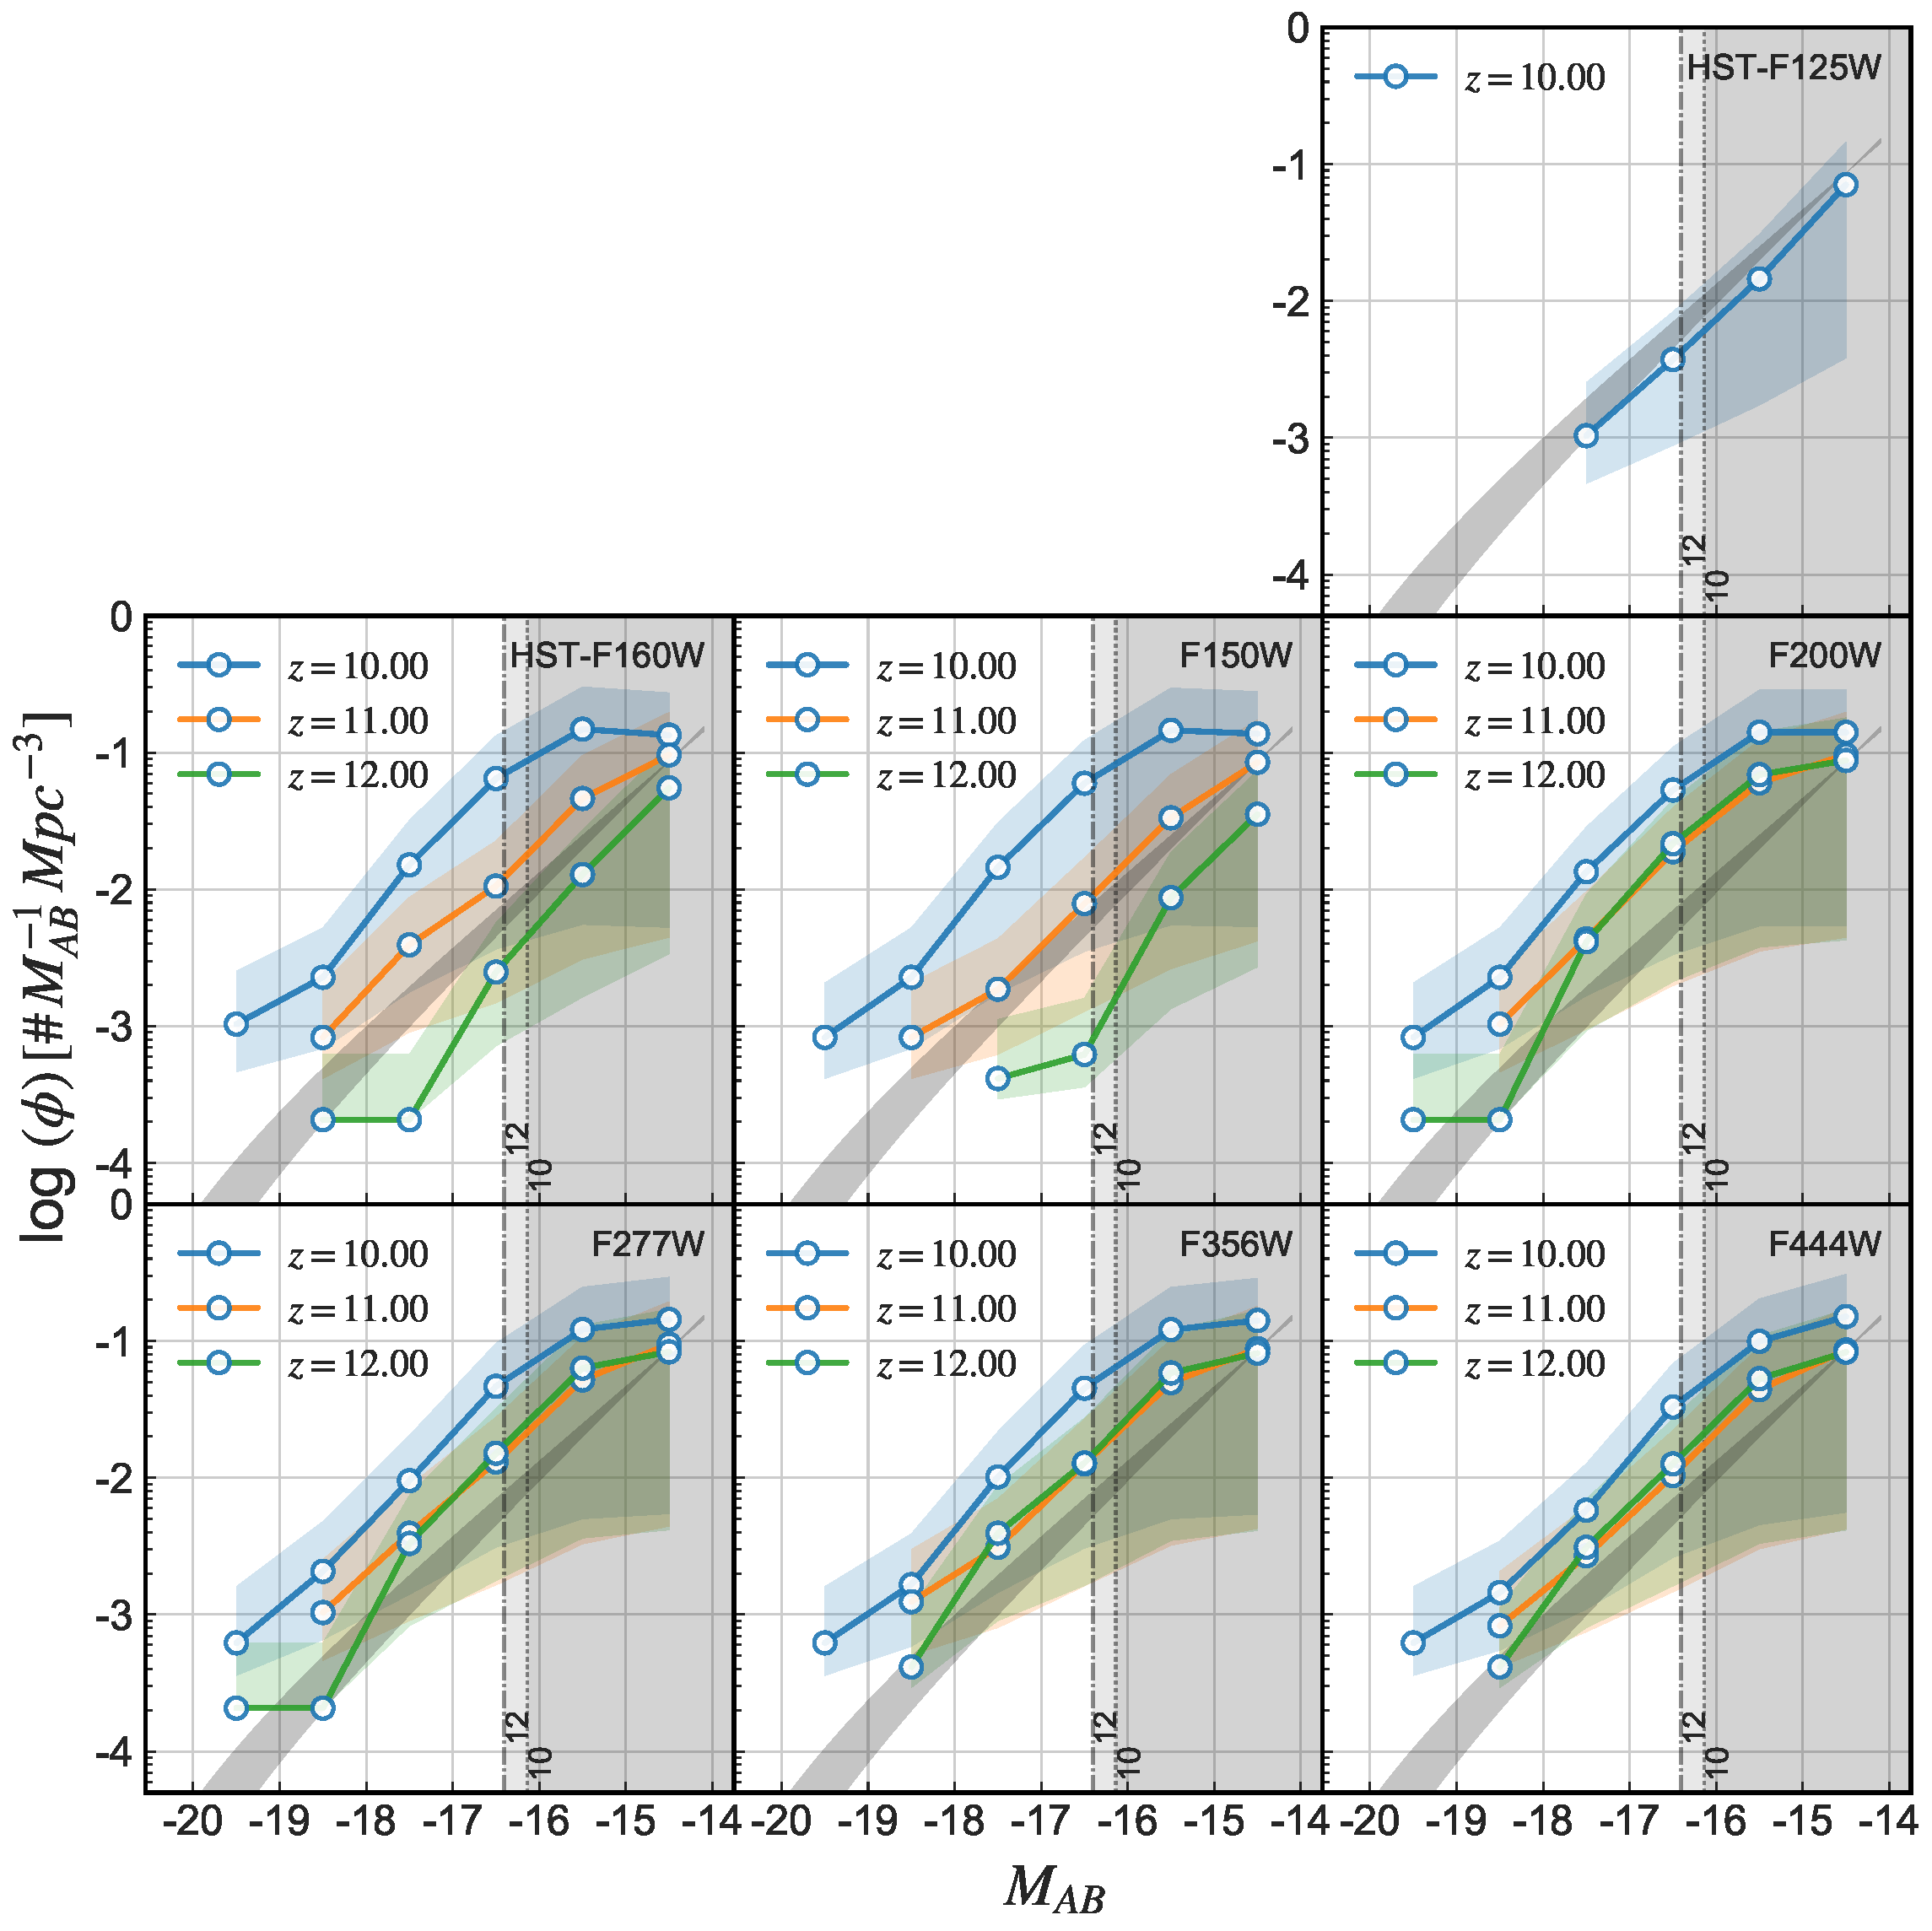
\includegraphics[width=2\columnwidth]{./filterLF1}
\caption{Luminosity functions, with 1$\sigma$ error bounds, derived from our simulated galaxies convolved with our filter models across the redshift range $10 \le z \le 12$. The dark grey Schechter functions represent the bounding redshifts and are again from \cite{2016PASA...33...37F} (without errors). The dark, vertical shaded areas of each plot indicate the regions where $m_{\rm AB} > 31.4$ mag, the JWST limiting magnitude for the ultra-deep campaign, for $z=10$ and $z=12$. If a redshift does not appear in a plot none of our galaxies were visible in that filter. Note that we have not included dust attenuation. }
\label{fig:filtLF1}
\end{center}
\end{figure*}

The remaining data, out to $z=12$, for the JWST filters are systematically higher than the predicted Schechter functions, although they are all within $1\sigma$ of the predictions. Interestingly, we do not see a significant difference between galaxies at $z=11$ and $z=12$ using filters centered at $2.0\mu$m (F200W) and redder. We note that all of these filters sample the rest-frame in the region bluer than Lyman-$\alpha$ in a region where we would expect maximal dust attenuation \citep{2001PASP..113.1449C}. This possibly explains part of the systematic brightness in relation to the predictions. In fact, a typical 1 mag reddening law would bring our LFs into good agreements with predictions. In particular, F200W and F277W sample the rest-frame flux from 0.18 $\mu$m to 0.21 $\mu$m -- where any dust absorption curve peaks. Filters F356W and F444W sample the rest-frame in the range $0.34\, \mu m \le \lambda \le 0.40\, \mu m$.

Figure \ref{fig:filtLF2} characterizes our LFs at $z\ge 13$. For this range of redshifts galaxies have to be brighter than $M_{\rm AB} < -16.5$ to be detected by JWST. Again we see our filter fluxes bracketing predictions. In fact, all of the remaining JWST filters redder than 2$\mu$m accumulate flux for our high-redshift galaxies, however none of our simulated galaxies at $z=16$ are detectable given our assumption of a limiting magnitude $m_{\rm AB} = 31.4$ mag. Of course, our relatively small simulation volume did not generate any of the more rare, yet bright, galaxies at these high redshifts. The flux trend, from lower-to-higher redshift follows expectations with galaxies appearing brighter at lower $z$.  However, only a small fraction of the simulated galaxies at the bright end of our data are observable by JWST.  While none of the filters detect galaxies at $z=16$, filters redder than 2 $\mu$m detect our galaxies out to $z=15$. Again, we note that our relatively small simulation box did not generate any of the more rare yet bright galaxies at these redshifts. Hence it is likely that these filters can detect these rare objects out to $z=16$ and possibly beyond.

\begin{figure*}[h]
\begin{center}
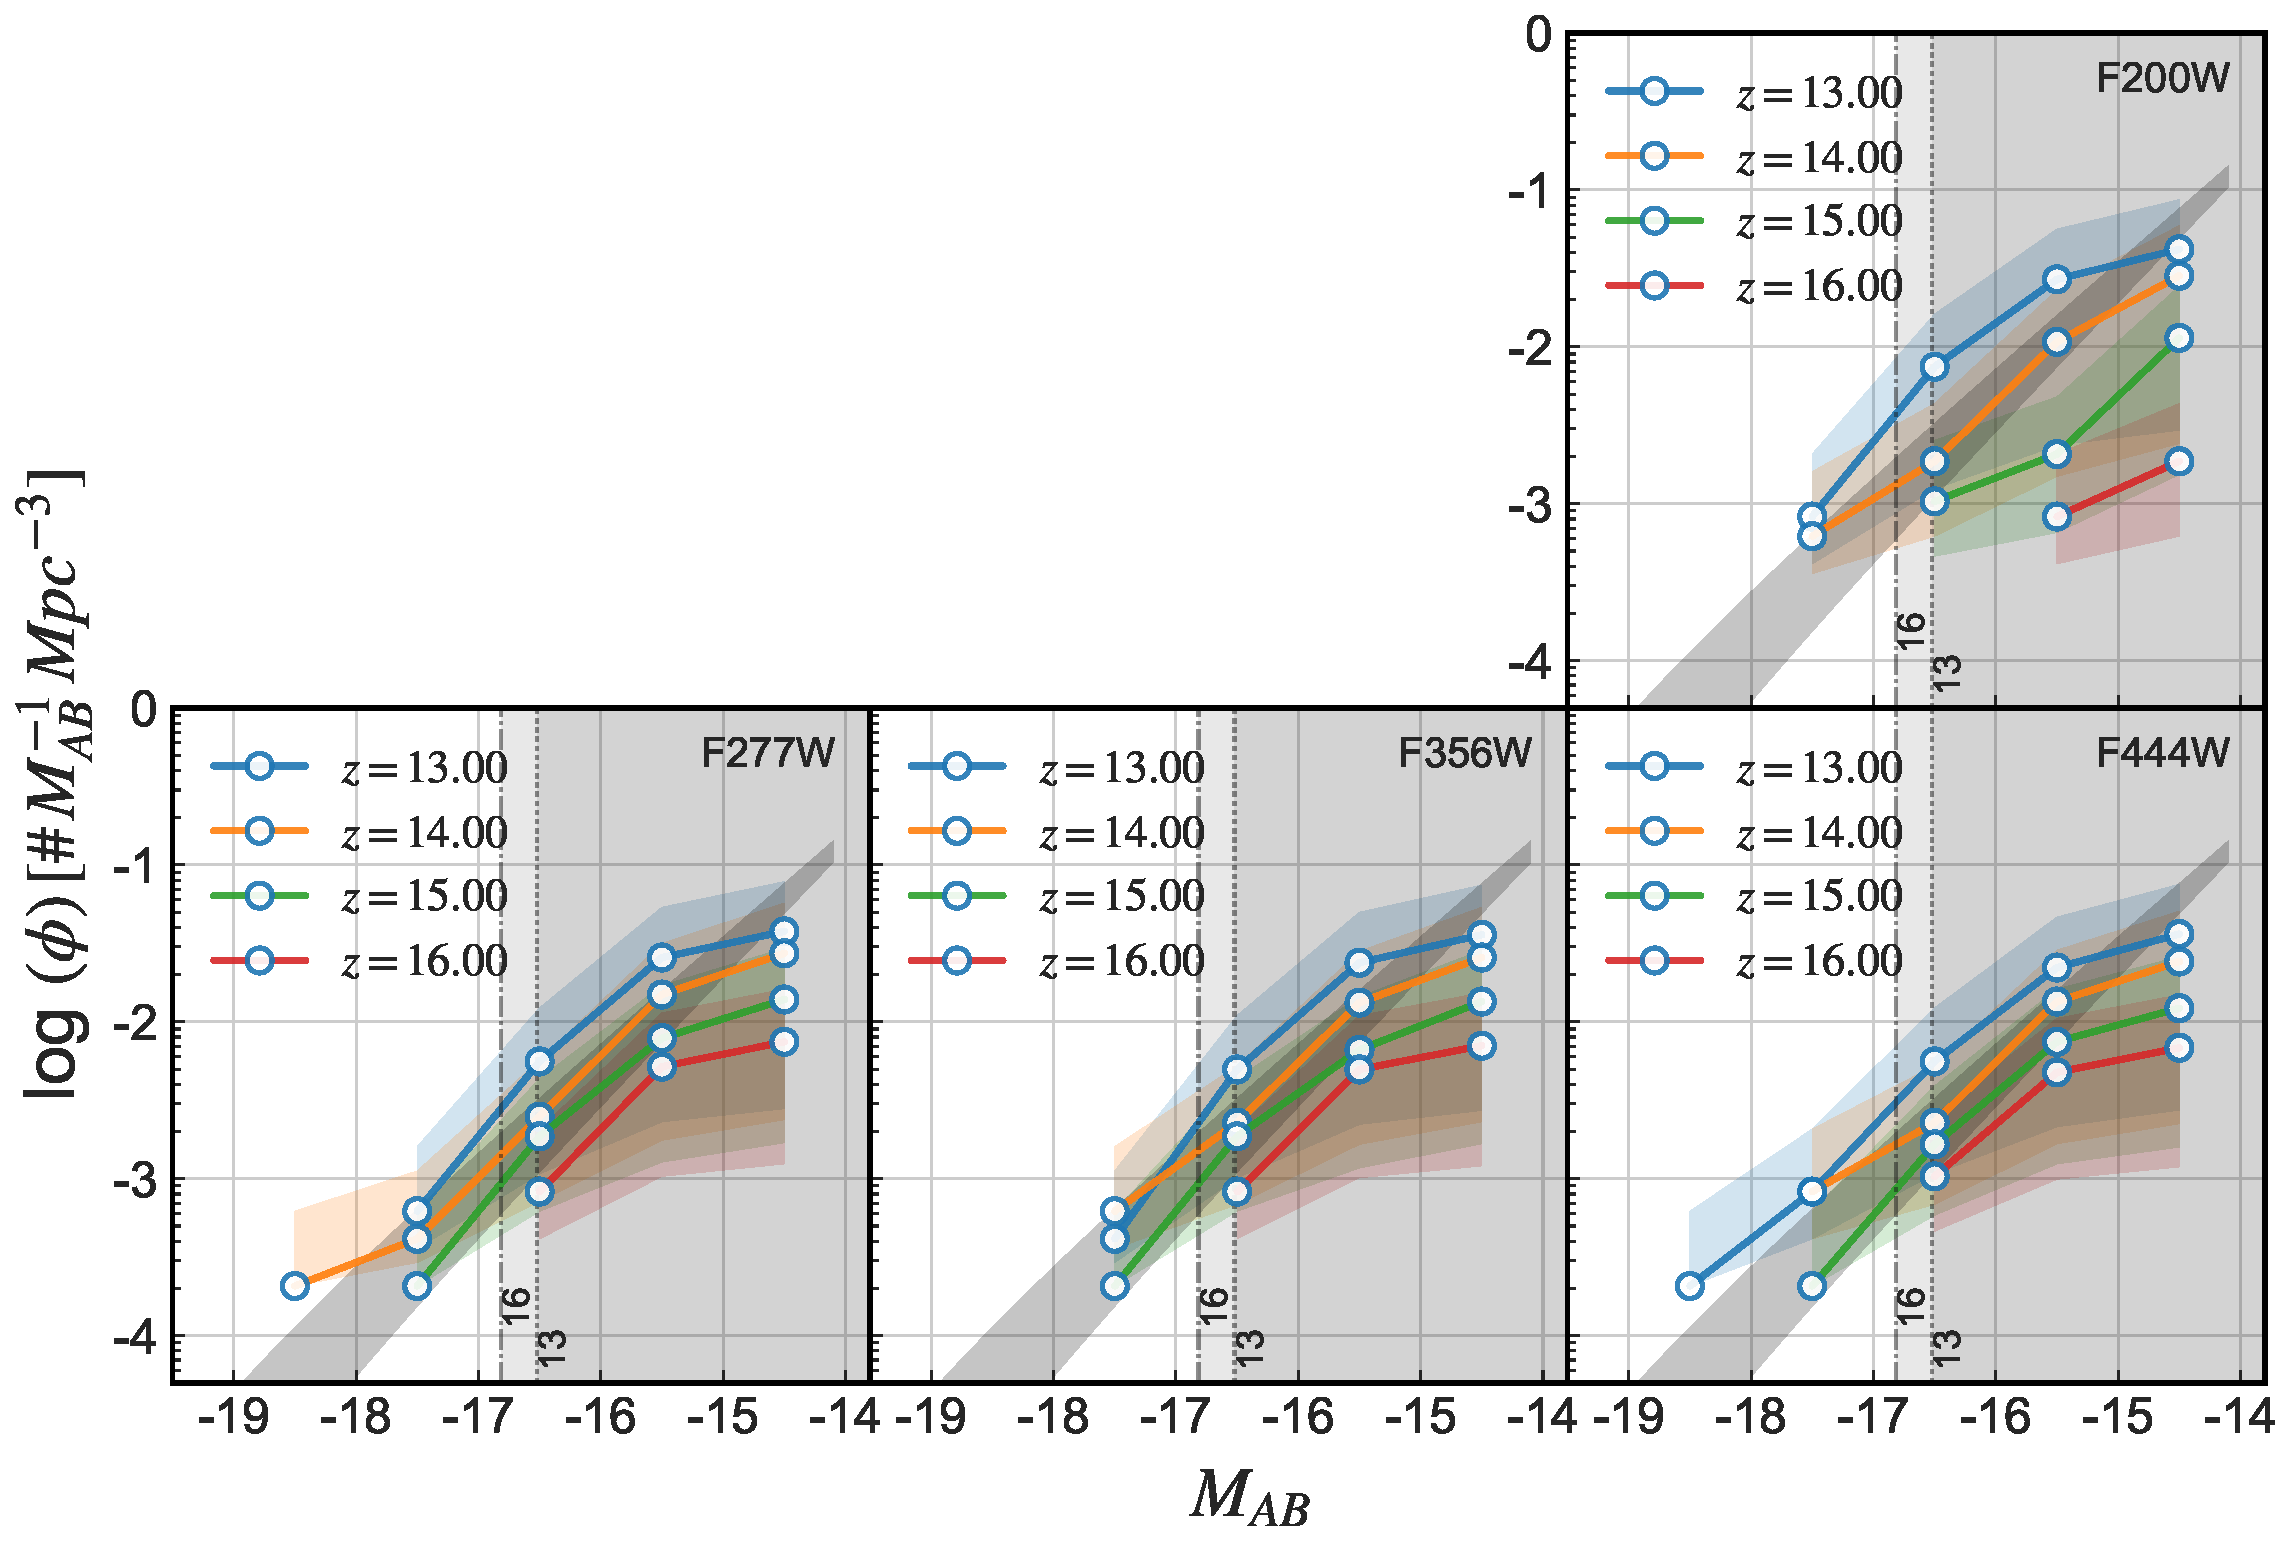
\includegraphics[width=2\columnwidth]{./filterLF2}
\caption{The same plots as in Figure \ref{fig:filtLF1} but for $13 \le z \le 16$. The vertical, grey shaded regions indicate where $m_{\rm AB} > 31.4$ mag for a noted redshift. The bounding Schechter functions are now for $z=13$ and 16. We note that all of our galaxies have dropped out of the Hubble filters.}
\label{fig:filtLF2}
\end{center}
\end{figure*}

%%%%%%%%%%%%%%
%%%%%%%%%%%%%%
\section{Conclusions}
We have used a large-scale cosmological simulation to study high-redshift galaxies and the prospect of finding Pop III-bright galaxies. While several of our contemporaries have done similar work \citep{2017arXiv170202146C, 2017arXiv170102749B, 2016MNRAS.462..235L, 2016ApJ...823..140X, 2015ApJ...807L..12O}, our approach is novel in that our models includes the enhancement to Pop III star formation we expect due to the timescale required to turbulently mix pollutants at subgrid scales. We find that our Pop III SFRD is approximately $2\times$ the rate we would have without modeling subgrid turbulent mixing. We have analyzed more than 20,000 galaxies in our simulation volume of 4828 comoving Mpc$^{3}$ producing UV LFs and statistics on the fraction of Pop III-bright galaxies across a range of redshifts. We have also generated LFs for several HST and JWST filters. 

The observational constraints on $z\ge 8$ LFs are uncertain at best \citep{2016PASA...33...37F, 2015MNRAS.450.3032M, 2015ApJ...803...34B, 2015ApJ...808..104O}.  Determining the faint-end slope, $\alpha$, is the challenge here since observations of galaxies dimmer than $M^{*}$ are likely to dominate galaxy number densities at high-redshift and, more importantly, to be the home of Pop III galaxies. We find that linear extrapolations of the faint-end slope to $z>8$, as captured in Table \ref{tab:schecParams}, appear valid to $z=16$.  While the Schechter function indicates an ever-increasing number of faint galaxies, we know that the actual LF must flatten and turn-over at some point. Even though the simulation's resolution limits our ability to estimate this turn-over magnitude, we have determined that galaxies down to $M_{\rm UV} = -14$ reasonably follow the extrapolated $\alpha$. Additionally, our simulation demonstrates that $M^{*}_{\rm UV}$, the absolute magnitude where galaxy counts begin an exponential decay, is brighter than $M_{\rm UV, AB} = -17$ out to $z=16$, again in agreement with linear extrapolations of current trends.

In the realm of Pop III-bright galaxies, we see a significant fraction of them at $z=12$ where almost 30\% of all galaxies brighter than $m_{UV} \le 31.4$ mag have 75\% or more of their flux coming from Pop III stars. While these galaxies are mostly out of reach for the HST, they should be observable via un-lensed JWST campaigns. As we look even farther back in cosmic time we predict that more than 40\% of observable galaxies will be Pop III-bright over the redshift range $13 \le z \le 14$. This is a rich era of Pop III galaxies. If we consider $10\times$ lensing -- out to $m_{UV} = 33$ mag -- we find slightly lower percentages of Pop III galaxies over $12 \le z \le 14$ due to the additional number of small, polluted galaxies that we encounter at this limiting magnitude. However, moving out to $z\ge15$ we again see very large fractions of Pop III-bright galaxies. In fact at $z=16$, 9 out-of 10 galaxies in our simulation are brighter than $m_{UV} \le 33$ mag and are also Pop III-bright. It is here that we truly enter the era of the very first galaxies.

Although our simulation's enhanced Pop III SFRD has no discernible impact on the LFs for $z \le 13$, and only minor implications for the LF at $z > 13$, it does play a significant role in the type of flux coming from our high redshift galaxies. We demonstrate that accurately modeling the Pop III stellar fraction is critical to determining the flux from these early galaxies. Even at lower redshift, between $8 \le z \le 13$, the fraction of Pop III-bright galaxies detectable decreases by 7\% if we do not consider subgrid turbulent mixing when determining the metallicity of star particles. 

Our LFs predict good news for JWST. Although we have not considered the effects of cosmic variance with regard to JWST's small fields-of-view \citep{2008ApJ...676..767T,2015ApJ...807L..12O}, our simulation exhibits galaxy counts per magnitude bin that exceed current, observationally-based predictions for filters redder than $\approx 1.6 \mu$m through $z=12$. At higher redshifts, $z \ge 13$, our predictions closely follow extrapolations of the Schechter function faint-end slope and indicate detections out to $z=15$ in filters $2.7 \mu$m and longer. In closing, we hope our results will help guide future searches for Pop III galaxies. 

%%%%%%%%%%%%%%
%%%%%%%%%%%%%%
\acknowledgments
We would like to thank Gabriela Huckabee for performing some of the research needed to reduce certain aspects of our simulation data. This work was supported in part by the National Science Foundation under Grant No. PHY-1430152 (JINA Center for the Evolution of the Elements) and by NASA theory grant NNX15AK82G. The simulations and much of the analysis for this work was carried out on the  NASA Pleiades supercomputer. We would also like to thank the NASA High-End Computing Capability support team.

%\appendix
%\section{Appendix}

\clearpage % Needed to ensure pictures are placed BEFORE the bibliography.
% Bibliography.
\pagebreak

\begin{thebibliography}{100}
\bibitem[Abel et al.(2002)]{2002Sci...295...93A} Abel, T., Bryan, G.~L., \& Norman, M.~L.\ 2002, Science, 295, 93
%\bibitem[An et al.(2013)]{2013ApJ...763...65A} An, D., Beers, T.~C., Johnson, J.~A., et al.\ 2013, \apj, 763, 65 
\bibitem[Aoki et al.(2006)]{2006ApJ...639..897A} Aoki, W., Frebel, A.,  Christlieb, N., et al.\ 2006, \apj, 639, 897 
%\bibitem[Asplund et  al.(2009)]{2009ARA&A..47..481A} Asplund, M., Grevesse, N., Sauval, A.~J., \& Scott, P.\ 2009, \araa, 47, 481 
\bibitem[Atek et al.(2015)]{2015ApJ...814...69A} Atek, H., Richard, J., Jauzac, M., et al.\ 2015, \apj, 814, 69 
\bibitem[Barrow et al.(2017)]{2017arXiv170102749B} Barrow, K.~S.~S., Wise, J.~H., Norman, M.~L., O'Shea, B.~W., \& Xu, H.\ 2017, arXiv:1701.02749 
\bibitem[Berry et al.(2012)]{2012ApJ...757..166B} Berry, M., Ivezi{\'c}, {\v Z}., Sesar, B., et al.\ 2012, \apj, 757, 166 
%\bibitem[Bouwens et al.(2012a)]{2012ApJ...752L...5B} Bouwens, R.~J., Illingworth, G.~D., Oesch, P.~A., et al.\ 2012, \apjl, 752, L5 
%\bibitem[Bouwens et al.(2012b)]{2012ApJ...754...83B} Bouwens, R.~J., Illingworth, G.~D., Oesch, P.~A., et al.\ 2012, \apj, 754, 83 
\bibitem[Bouwens et al.(2014)]{2014ApJ...795..126B} Bouwens, R.~J., Bradley, L., Zitrin, A., et al.\ 2014, \apj, 795, 126 
\bibitem[Bouwens et al.(2015)]{2015ApJ...803...34B} Bouwens, R.~J., Illingworth, G.~D., Oesch, P.~A., et al.\ 2015, \apj, 803, 34 
\bibitem[Bouwens et al.(2016)]{2016ApJ...830...67B} Bouwens, R.~J., Oesch, P.~A., Labb{\'e}, I., et al.\ 2016, \apj, 830, 67 
\bibitem[Bowler et al.(2016)]{2016arXiv160900727B} Bowler, R.~A.~A., McLure, R.~J., Dunlop, J.~S., et al.\ 2016, arXiv:1609.00727 
\bibitem[Bromm et al.(2002)]{2002ApJ...564...23B} Bromm, V., Coppi, P.~S.,  \& Larson, R.~B.\ 2002, \apj, 564, 23
\bibitem[Bromm  \& Loeb(2003)]{2003Natur.425..812B} Bromm, V., \& Loeb, A.\ 2003, \nat, 425, 812
\bibitem[Bromm \& Larson(2004)]{2004ARA&A..42...79B} Bromm, V., \& Larson, R.~B.\ 2004, \araa, 42, 79 
\bibitem[Bromm(2013)]{2013IAUS..295....3B} Bromm, V.\ 2013, The Intriguing Life of Massive Galaxies, 295, 3 
\bibitem[Bromm(2014)]{2014MmSAI..85..202B} Bromm, V.\ 2014, \memsai, 85, 202 
\bibitem[Brook et al.(2007)]{2007ApJ...661...10B} Brook, C.~B., Kawata, D.,  Scannapieco, E., Martel, H., \& Gibson, B.~K.\ 2007, \apj, 661, 10 
\bibitem[Caffau et al.(2011)]{2011Natur.477...67C} Caffau, E., Bonifacio, P., Fran{\c c}ois, P., et al.\ 2011, \nat, 477, 67 
\bibitem[Calzetti(2001)]{2001PASP..113.1449C} Calzetti, D.\ 2001, \pasp, 113, 1449 
\bibitem[Cassata et  al.(2013)]{2013A&A...556A..68C} Cassata, P., Le F{\`e}vre, O., Charlot, S., et al.\ 2013, \aap, 556, A68 
\bibitem[Cayrel et al.(2004)]{2004A&A...416.1117C} Cayrel, R., Depagne, E., Spite, M., et al.\ 2004, \aap, 416, 1117 
%\bibitem[Chai  \& Mahesh(2012)]{2012JFM...699..385C} Chai, X., \& Mahesh, K.\ 2012, Journal of Fluid Mechanics, 699, 385
\bibitem[Christlieb et al.(2002)]{2002Natur.419..904C} Christlieb, N., Bessell, M.~S., Beers, T.~C., et al.\ 2002, \nat, 419, 904 
%\bibitem[Clark et al.(2011)]{2011ApJ...727..110C} Clark, P.~C., Glover, S.~C.~O., Klessen, R.~S., \& Bromm, V.\ 2011, \apj, 727, 110 
%\bibitem[Codis et al.(2015)]{2015MNRAS.448.3391C} Codis, S., Gavazzi, R.,  Dubois, Y., et al.\ 2015, \mnras, 448, 3391 
\bibitem[Coe et al.(2013)]{2013ApJ...762...32C} Coe, D., Zitrin, A., Carrasco, M., et al.\ 2013, \apj, 762, 32 
%\bibitem[Cooke \& Madau(2014)]{2014ApJ...791..116C} Cooke, R.~J., \& Madau, P.\ 2014, \apj, 791, 116 
\bibitem[Cowley et al.(2017)]{2017arXiv170202146C} Cowley, W., Baugh, C., Cole, S., Frenk, C., \& Lacey, C.\ 2017, arXiv:1702.02146 
\bibitem[Crosby et al.(2013)]{2013ApJ...773..108C} Crosby, B.~D., O'Shea,  B.~W., Smith, B.~D., Turk, M.~J., \& Hahn, O.\ 2013, \apj, 773, 108 
%\bibitem[Curl(1963)]{1963Curl} Curl, S. 1963,  AIChE J.,  9, 175
\bibitem[Dawson et al.(2004)]{2004ApJ...617..707D} Dawson, S., Rhoads,  J.~E., Malhotra, S., et al.\ 2004, \apj, 617, 707 
\bibitem[Deharveng et al.(2010)]{2010A&A...523A...6D} Deharveng, L., Schuller, F., Anderson, L.~D., et al.\ 2010, \aap, 523, A6 
\bibitem[Dijkstra \& Wyithe(2007)]{2007MNRAS.379.1589D} Dijkstra, M., \& Wyithe, J.~S.~B.\ 2007, \mnras, 379, 1589 
%\bibitem[Dopazo(1979)]{1979PhFl...22...20D} Dopazo, C.\ 1979, Physics of Fluids, 22, 20
%\bibitem[Dubois \& Teyssier(2008)]{2008A&A...477...79D} Dubois, Y., \& Teyssier, R.\ 2008, \aap, 477, 79 
%\bibitem[Duplat \& Villermaux(2008)]{2008JFM...617...51D} Duplat, J., \& Villermaux, E.\ 2008, Journal of Fluid Mechanics, 617, 51 
\bibitem[Frebel et al.(2005)]{2005Natur.434..871F} Frebel, A., Aoki, W., Christlieb, N., et al.\ 2005, \nat, 434, 871
\bibitem[Einfeldt(1988)]{1988SJNA...25..294E} Einfeldt, B.\ 1988, SIAM  Journal on Numerical Analysis, 25, 294 
\bibitem[Eisenstein \& Hut(1998)]{1998ApJ...498..137E} Eisenstein, D.~J., \& Hut, P.\ 1998, \apj, 498, 137 
%\bibitem[Erlebacher et al.(1992)]{1992JFM...238..155E} Erlebacher, G.,  Hussaini, M.~Y., Speziale, C.~G.,  \& Zang, T.~A.\ 1992, Journal of Fluid Mechanics, 238, 155 
%\bibitem[Federrath et al.(2010)]{2010A&A...512A..81F} Federrath, C., Roman-Duval, J., Klessen, R.~S., Schmidt, W., \& Mac Low, M.-M.\ 2010, \aap, 512, A81
\bibitem[Finkelstein(2016)]{2016PASA...33...37F} Finkelstein, S.~L.\ 2016, \pasa, 33, e037 
\bibitem[Gardner et al. (2006)]{2016jwst} Gardner, J.P., Mather, J.C., Clampin, M. et al. Space Sci Rev (2006) 123: 485. doi:10.1007/s11214-006-8315-7
%\bibitem[Genin  \& Menon(2010)]{2010JTurb..11....4G} Genin, F., \& Menon, S.\ 2010, Journal of Turbulence, 11, N4
%\bibitem[Ghosal et al.(1995)]{1995JFM...286..229G} Ghosal, S., Lund, T.~S.,  Moin, P., \& Akselvoll, K.\ 1995, Journal of Fluid Mechanics, 286, 229 
\bibitem[Girardi et al.(2000)]{2000A&AS..141..371G} Girardi, L., Bressan, A., Bertelli, G., \& Chiosi, C.\ 2000, \aaps, 141, 371 
%\bibitem[Greif  \& Bromm(2006)]{2006MNRAS.373..128G} Greif, T.~H., \& Bromm, V.\ 2006, \mnras, 373, 128 
\bibitem[Greif et al.(2010)]{2010ApJ...716..510G} Greif, T.~H., Glover,  S.~C.~O., Bromm, V., \& Klessen, R.~S.\ 2010, \apj, 716, 510
%\bibitem[Greif et al.(2012)]{2012MNRAS.424..399G} Greif, T.~H., Bromm, V.,  Clark, P.~C., et al.\ 2012, \mnras, 424, 399
\bibitem[Guillet \& Teyssier(2011)]{GT2011} Guillet, T., Chapon,  D., \& Teyssier, R.\ 2011, Journal of Computational Physics, 230, 4756 
%\bibitem[Guillet et al.(2013)]{2013ascl.soft10002G} Guillet, T., Chapon,  D., \& Labadens, M.\ 2013, Astrophysics Source Code Library, 10002 
%\bibitem[Haardt \& Madau(1996)]{1996ApJ...461...20H} Haardt, F., \& Madau, P.\ 1996, \apj, 461, 20 
%\bibitem[Hansen et al.(2015)]{2015arXiv151107812H} Hansen, C.~J., Nordstroem, B., Hansen, T.~T., et al.\ 2015, arXiv:1511.07812 
\bibitem[Hartwig et al.(2015)]{2015MNRAS.447.3892H} Hartwig, T., Bromm, V., Klessen, R.~S., \& Glover, S.~C.~O.\ 2015, \mnras, 447, 3892 
%\bibitem[Heger \& Woosley(2002)]{2002ApJ...567..532H} Heger, A., \& Woosley, S.~E.\ 2002, \apj, 567, 532 
%\bibitem[Heger(2016)]{hegerwebsite} Heger, A., StarFit�,\ 2016, \texttt{http://starfit.org/}
%\bibitem[Hirano \& Yoshida(2013)]{2013ApJ...763...52H} Hirano, S., \& Yoshida, N.\ 2013, \apj, 763, 52 
%\bibitem[Hirano et al.(2014)]{2014ApJ...781...60H} Hirano, S., Hosokawa,  T., Yoshida, N., et al.\ 2014, \apj, 781, 60 
%\bibitem[Hosokawa et al.(2011)]{2011Sci...334.1250H} Hosokawa, T., Omukai, K., Yoshida, N., \& Yorke, H.~W.\ 2011, Science, 334, 1250 
\bibitem[Howes et al.(2015)]{2015Natur.527..484H} Howes, L.~M., Casey, A.~R., Asplund, M., et al.\ 2015, \nat, 527, 484
%\bibitem[Hutchins(1976)]{1976ApJ...205..103H} Hutchins, J.~B.\ 1976, \apj,  205, 103 
%\bibitem[Inoue(2011)]{2011MNRAS.415.2920I} Inoue, A.~K.\ 2011, \mnras, 415, 2920 
%\bibitem[Ishigaki et al.(2014)]{2014ApJ...792L..32I} Ishigaki, M.~N., Tominaga, N., Kobayashi, C., \& fto, K.\ 2014, \apjl, 792, L32 
\bibitem[Ishigaki et al.(2017)]{2017arXiv170204867I} Ishigaki, M., Kawamata, R., Ouchi, M., Oguri, M., \& Shimasaku, K.\ 2017, arXiv:1702.04867 
\bibitem[Ishiyama et al.(2016)]{2016arXiv160200465I} Ishiyama, T., Sudo,  K., Yokoi, S., et al.\ 2016, arXiv:1602.00465 
%\bibitem[Janicka et al.(1979)]{1979JNET....4...47J} Janicka, J., Kolbe, W., \& Kollmann, W.\ 1979, Journal of Non Equilibrium Thermodynamics, 4, 47 
%\bibitem[Jeon et al.(2014)]{2014MNRAS.444.3288J} Jeon, M., Pawlik, A.~H., Bromm, V., \& Milosavljevi{\'c}, M.\ 2014, \mnras, 444, 3288 
\bibitem[Jimenez \& Haiman(2006)]{2006Natur.440..501J} Jimenez, R., \& Haiman, Z.\ 2006, \nat, 440, 501
%\bibitem[Johnson \& Bromm(2006)]{2006MNRAS.366..247J} Johnson, J.~L., \& Bromm, V.\ 2006, \mnras, 366, 247
\bibitem[Johnson et al.(2013)]{2013MNRAS.428.1857J} Johnson, J.~L., Dalla Vecchia, C., \& Khochfar, S.\ 2013, \mnras, 428, 1857 
\bibitem[Kashikawa et al.(2012)]{2012ApJ...761...85K} Kashikawa, N., Nagao,  T., Toshikawa, J., et al.\ 2012, \apj, 761, 85 
\bibitem[Keller et al.(2014)]{2014Natur.506..463K} Keller, S.~C., Bessell, M.~S., Frebel, A., et al.\ 2014, \nat, 506, 463 
%\bibitem[Kennicutt(1998)]{1998ARA&A..36..189K} Kennicutt, R.~C., Jr.\ 1998, \araa, 36, 189 
%\bibitem[Kim et al.(2014)]{2014ApJS..210...14K} Kim, J.-h., Abel, T., Agertz, O., et al.\ 2014, \apjs, 210, 14 
\bibitem[Koekemoer et al.(2013)]{2013ApJS..209....3K} Koekemoer, A.~M., Ellis, R.~S., McLure, R.~J., et al.\ 2013, \apjs, 209, 3 
%\bibitem[Krumholz \& Tan(2007)]{2007ApJ...654..304K} Krumholz, M.~R., \& Tan, J.~C.\ 2007, \apj, 654, 304
\bibitem[Larson et al.(2011)]{2011ApJS..192...16L} Larson, D., Dunkley, J., Hinshaw, G., et al.\ 2011, \apjs, 192, 16 
\bibitem[Leitherer et al.(2014)]{2014ApJS..212...14L} Leitherer, C., Ekstr{\"o}m, S., Meynet, G., et al.\ 2014, \apjs, 212, 14 
\bibitem[Liu et al.(2016)]{2016MNRAS.462..235L} Liu, C., Mutch, S.~J., Angel, P.~W., et al.\ 2016, \mnras, 462, 235 
\bibitem[Livermore et al.(2017)]{2017ApJ...835..113L} Livermore, R.~C., Finkelstein, S.~L., \& Lotz, J.~M.\ 2017, \apj, 835, 113 
\bibitem[Ma et al.(2016)]{2016MNRAS.456.2140M} Ma, X., Hopkins, P.~F., Faucher-Gigu{\`e}re, C.-A., et al.\ 2016, \mnras, 456, 2140 
\bibitem[Madau(1995)]{1995ApJ...441...18M} Madau, P.\ 1995, \apj, 441, 18 
\bibitem[Madau \& Dickinson(2014)]{2014ARA&A..52..415M} Madau, P., \& Dickinson, M.\ 2014, \araa, 52, 415
\bibitem[Maio et al.(2010)]{2010MNRAS.407.1003M} Maio, U., Ciardi, B., Dolag, K., Tornatore, L., \& Khochfar, S.\ 2010, \mnras, 407, 1003 
\bibitem[Malhotra  \& Rhoads(2002)]{2002ApJ...565L..71M} Malhotra, S., \& Rhoads, J.~E.\ 2002, \apjl, 565, L71 
\bibitem[Maiolino et al.(2008)]{2008A&A...488..463M} Maiolino, R., Nagao, T., Grazian, A., et al.\ 2008, \aap, 488, 463 
%\bibitem[Martin et al.(1996)]{1996ApJ...461..265M} Martin, P.~G., Schwarz, D.~H., \& Mandy, M.~E.\ 1996, \apj, 461, 265 
\bibitem[Mashian et al.(2016)]{2016MNRAS.455.2101M} Mashian, N., Oesch, P.~A., \& Loeb, A.\ 2016, \mnras, 455, 2101 
\bibitem[Mason et al.(2015)]{2015ApJ...813...21M} Mason, C.~A., Trenti, M., \& Treu, T.\ 2015, \apj, 813, 21 
\bibitem[Mason et al.(2016)]{2016ApJ...816...46M} Mason, C.~A., Trenti, M., \& Treu, T.\ 2016, \apj, 816, 46 
%\bibitem[McKee  \& Tan(2008)]{2008ApJ...681..771M} McKee, C.~F., \& Tan, J.~C.\ 2008, \apj, 681, 771 
\bibitem[McLeod et al.(2015)]{2015MNRAS.450.3032M} McLeod, D.~J., McLure, R.~J., Dunlop, J.~S., et al.\ 2015, \mnras, 450, 3032 
%\bibitem[Moeng(1984)]{1984JAtS...41.2052M} Moeng, C.-H.\ 1984, Journal of  Atmospheric Sciences, 41, 2052 
%\bibitem[Moin et al.(1991)]{1991PhFl....3.2746M} Moin, P., Squires, K.,  Cabot, W., \& Lee, S.\ 1991, Physics of Fluids, 3, 2746 
\bibitem[Nagao et al.(2008)]{2008ApJ...680..100N} Nagao, T., Sasaki, S.~S.,  Maiolino, R., et al.\ 2008, \apj, 680, 100 
\bibitem[Norris et al.(2007)]{2007ApJ...670..774N} Norris, J.~E.,  Christlieb, N., Korn, A.~J., et al.\ 2007, \apj, 670, 774 
%\bibitem[Norris et al.(2013)]{2013ApJ...762...28N} Norris, J.~E., Yong, D.,  Bessell, M.~S., et al.\ 2013, \apj, 762, 28
\bibitem[Oesch et al.(2013)]{2013ApJ...773...75O} Oesch, P.~A., Bouwens, R.~J., Illingworth, G.~D., et al.\ 2013, \apj, 773, 75 
\bibitem[Oesch et al.(2015)]{2015ApJ...808..104O} Oesch, P.~A., Bouwens, R.~J., Illingworth, G.~D., et al.\ 2015, \apj, 808, 104 
\bibitem[Oke \& Gunn(1983)]{1983ApJ...266..713O} Oke, J.~B., \& Gunn, J.~E.\ 1983, \apj, 266, 713 
\bibitem[Omukai et al.(2005)]{2005ApJ...626..627O} Omukai, K., Tsuribe, T., Schneider, R., \& Ferrara, A.\ 2005, \apj, 626, 627 
\bibitem[O'Shea et al.(2015)]{2015ApJ...807L..12O} O'Shea, B.~W., Wise, J.~H., Xu, H., \& Norman, M.~L.\ 2015, \apjl, 807, L12 
\bibitem[O'Shea  \& Norman(2007)]{2007ApJ...654...66O} O'Shea, B.~W., \& Norman, M.~L.\ 2007, \apj, 654, 66 
%\bibitem[O'Shea et al.(2015)]{2015ApJ...807L..12O} O'Shea, B.~W., Wise, J.~H., Xu, H., \& Norman, M.~L.\ 2015, \apjl, 807, L12
\bibitem[Pacucci et al.(2017)]{2017MNRAS.468L..77P} Pacucci, F., Pallottini, A., Ferrara, A., \& Gallerani, S.\ 2017, \mnras, 468, L77 
\bibitem[Paardekooper et al.(2013)]{2013MNRAS.429L..94P} Paardekooper, J.-P., Khochfar, S., \& Dalla Vecchia, C.\ 2013, \mnras, 429, L94 
%\bibitem[Padoan et al.(2007)]{2007ApJ...661..972P} Padoan, P., Nordlund, {\AA}., Kritsuk, A.~G., Norman, M.~L., \& Li, P.~S.\ 2007, \apj, 661, 972 
%\bibitem[Padoan et al.(2016)]{2016ApJ...822...11P} Padoan, P., Pan, L., Haugb{\o}lle, T., \& Nordlund, {\AA}.\ 2016, \apj, 822, 11 
\bibitem[Pallottini et al.(2014)]{2014MNRAS.440.2498P} Pallottini, A.,  Ferrara, A., Gallerani, S., Salvadori, S.,  \& D'Odorico, V.\ 2014, \mnras, 440, 2498 
\bibitem[Pan \& Scalo(2007)]{2007ApJ...654L..29P} Pan, L., \& Scalo, J.\ 2007, \apjl, 654, L29 
%\bibitem[Pan \& Scannapieco(2011)]{2011PhRvE..83d5302P} Pan, L., \& Scannapieco, E.\ 2011, \pre, 83, 045302 
\bibitem[Pan et al.(2012)]{2012JFM...700..459P} Pan, L., Scannapieco, E., \& Scalo, J.\ 2012, JFM, 700, 459 
\bibitem[Pan et al.(2013)]{2013ApJ...775..111P} Pan, L., Scannapieco, E., \& Scalo, J.\ 2013, \apj, 775, 111 
%\bibitem[Piau et al.(2006)]{2006ApJ...653..300P} Piau, L., Beers, T.~C., Balsara, D.~S., et al.\ 2006, \apj, 653, 300 
\bibitem[Planck Collaboration et al.(2015)]{2015arXiv150201589P} Planck Collaboration, Ade, P.~A.~R., Aghanim, N., et al.\ 2015, arXiv:1502.01589 
%\bibitem[Prieto et al.(2008)]{2008arXiv0809.2786P} Prieto, J.~P., Infante,  L., \& Jimenez, R.\ 2008, arXiv:0809.2786 
%% The 'Pop. III stars from turbulent fragmentation at redshift ~ 11' paper
%\bibitem[Prieto et al.(2011)]{arXiv:1101.5163} Prieto, J.~P.,  Padoan, P. , Infante,  L., \& Jimenez, R.\ 2011, arXiv:1101.5163 
%\bibitem[Pontzen et al.(2013)]{2013ascl.soft05002P} Pontzen, A., Ro{\v s}kar, R., Stinson, G., \& Woods, R.\ 2013, Astrophysics Source Code Library, 1305.002 
\bibitem[Prunet et al.(2008)]{2008ApJS..178..179P} Prunet, S., Pichon, C., Aubert, D., et al.\ 2008, \apjs, 178, 179
\bibitem[Raiter et al.(2010)]{2010A&A...523A..64R} Raiter, A., Schaerer, D., \& Fosbury, R.~A.~E.\ 2010, \aap, 523, A64 
%\bibitem[Rasera \& Teyssier(2006)]{2006A&A...445....1R} Rasera, Y., \& Teyssier, R.\ 2006, \aap, 445, 1 
%\bibitem[Raskin et al.(2008)]{2008ApJ...689..358R} Raskin, C., Scannapieco, E., Rhoads, J., \& Della Valle, M.\ 2008, \apj, 689, 358 
%\bibitem[Reed et al.(2005)]{2005MNRAS.363..393R} Reed, D.~S., Bower, R., Frenk, C.~S., et al.\ 2005, \mnras, 363, 393 
\bibitem[Richardson et al.(2013)]{2013ApJ...771...81R} Richardson,  M.~L.~A., Scannapieco, E., \& Thacker, R.~J.\ 2013, \apj, 771, 81 
\bibitem[Ritter et al.(2015)]{2015MNRAS.451.1190R} Ritter, J.~S., Sluder,  A., Safranek-Shrader, C., Milosavljevi{\'c}, M.,  \& Bromm, V.\ 2015, \mnras, 451, 1190 
\bibitem[Salpeter(1955)]{1955ApJ...121..161S} Salpeter, E.~E.\ 1955, \apj, 121, 161 
\bibitem[Salvadori et al.(2010)]{2010MNRAS.401L...5S} Salvadori, S.,  Ferrara, A., Schneider, R., Scannapieco, E.,  \& Kawata, D.\ 2010, \mnras, 401, L5
\bibitem[Sarmento et al.(2017)]{2017ApJ...834...23S} Sarmento, R., Scannapieco, E., \& Pan, L.\ 2017, \apj, 834, 23 
\bibitem[Scannapieco et al.(2003)]{2003ApJ...589...35S} Scannapieco, E., Schneider, R., \& Ferrara, A.\ 2003, \apj, 589, 35 
%\bibitem[Scannapieco(2005)]{2005ApJ...624L...1S} Scannapieco, E.\ 2005, \apjl, 624, L1
\bibitem[Scannapieco et al.(2006)]{2006ApJ...653..285S} Scannapieco, E., Kawata, D., Brook, C.~B., et al.\ 2006, \apj, 653, 285 
%\bibitem[Scannapieco  \& Br{\"u}ggen(2010)]{2010MNRAS.405.1634S} Scannapieco, E., \& Br{\"u}ggen, M.\ 2010, \mnras, 405, 1634 
\bibitem[Scannapieco \& Oh(2004)]{2004AAS...205.9421S} Scannapieco, E., \& Oh, P.\ 2004, Bulletin of the American Astronomical Society, 36, 94.21 
\bibitem[Schaerer(2002)]{2002A&A...382...28S} Schaerer, D.\ 2002, \aap, 382, 28 
\bibitem[Schaerer(2003)]{2003A&A...397..527S} Schaerer, D.\ 2003, \aap, 397, 527 
\bibitem[Schaerer et al.(2015)]{2015A&A...574A..19S} Schaerer, D., Boone, F., Zamojski, M., et al.\ 2015, \aap, 574, A19 
%\bibitem[Schaerer(2002)]{2002A&A...382...28S} Schaerer, D.\ 2002, \aap, 382, 28 
%\bibitem[Schaye et al.(2015)]{2015MNRAS.446..521S} Schaye, J., Crain,  R.~A., Bower, R.~G., et al.\ 2015, \mnras, 446, 521 
\bibitem[Schechter(1976)]{1976ApJ...203..297S} Schechter, P.\ 1976, \apj, 203, 297 
\bibitem[Schneider et al.(2003)]{2003Natur.422..869S} Schneider, R., Ferrara, A., Salvaterra, R., Omukai, K., \& Bromm, V.\ 2003, \nat, 422, 869 
%\bibitem[Schmidt(1959)]{1959ApJ...129..243S} Schmidt, M.\ 1959, \apj, 129,  243 
%\bibitem[Schmidt et  al.(2006)]{2006A&A...450..265S} Schmidt, W., Niemeyer, J.~C., \& Hillebrandt, W.\ 2006, \aap, 450, 265 
%\bibitem[Schumann(1975)]{1975JCoPh..18..376S} Schumann, U.\ 1975, Journal  of Computational Physics, 18, 376  
%\bibitem[Sluder et al.(2016)]{2016MNRAS.456.1410S} Sluder, A., Ritter, J.~S., Safranek-Shrader, C., Milosavljevi{\'c}, M., \& Bromm, V.\ 2016, \mnras, 456, 1410 
%\bibitem[Smagorinsky(1963)]{1963MWRv...91...99S} Smagorinsky, J.\ 1963, Monthly Weather Review, 91, 99 \& Woods, R.\ 2013, Astrophysics Source Code Library, 5002 
\bibitem[Sobral et al.(2015)]{2015ApJ...808..139S} Sobral, D., Matthee, J.,  Darvish, B., et al.\ 2015, \apj, 808, 139 
\bibitem[Somerville et al.(2008)]{2008MNRAS.391..481S} Somerville, R.~S., Hopkins, P.~F., Cox, T.~J., Robertson, B.~E., \& Hernquist, L.\ 2008, \mnras, 391, 481 
%\bibitem[Spitzer(1956)]{1956pfig.book.....S} Spitzer, L.\ 1956, Physics of  Fully Ionized Gases, New York: Interscience Publishers, 1956,  
%\bibitem[Stacy et al.(2010)]{2010MNRAS.403...45S} Stacy, A., Greif, T.~H.,  \& Bromm, V.\ 2010, \mnras, 403, 45
%\textbf{\bibitem[Sur et al.(2014)]{2014ApJ...784...94S} Sur, S., Pan, L., \& Scannapieco, E.\ 2014, \apj, 784, 94 }
\bibitem[Somerville et al.(2008)]{2008MNRAS.391..481S} Somerville, R.~S., Hopkins, P.~F., Cox, T.~J., Robertson, B.~E., \& Hernquist, L.\ 2008, \mnras, 391, 481 
%\bibitem[Sutherland \& Dopita(1993)]{1993ApJS...88..253S} Sutherland, R.~S., \& Dopita, M.~A.\ 1993, \apjs, 88, 253 
\bibitem[Teyssier(2002)]{2002A&A...385..337T} Teyssier, R.\ 2002, \aap, 385, 337 
%\bibitem[Teyssier(2015)]{Teyssier UV} Teyssier, R., Private communication 
%\bibitem[Timmes(2016)]{Timmes} Timmes, F. X.\ 2016, Private communication
\bibitem[Tornatore et al.(2007)]{2007MNRAS.382..945T} Tornatore, L., Ferrara, A., \& Schneider, R.\ 2007, \mnras, 382, 945 
\bibitem[Trenti \& Shull(2010)]{2010ApJ...712..435T} Trenti, M., \& Shull, J.~M.\ 2010, \apj, 712, 435 
\bibitem[Trenti \& Stiavelli(2008)]{2008ApJ...676..767T} Trenti, M., \& Stiavelli, M.\ 2008, \apj, 676, 767-780 
\bibitem[Tremblin et al.(2012)]{2012A&A...546A..33T} Tremblin, P., Audit, E., Minier, V., Schmidt, W., \& Schneider, N.\ 2012, \aap, 546, A33 
\bibitem[Tumlinson et al.(2001)]{2001ApJ...550L...1T} Tumlinson, J., Giroux, M.~L., \& Shull, J.~M.\ 2001, \apjl, 550, L1 
\bibitem[Tumlinson(2006)]{2006ApJ...641....1T} Tumlinson, J.\ 2006, \apj,  641, 1
%\bibitem[Turk et al.(2009)]{2009Sci...325..601T} Turk, M.~J., Abel, T., \& O'Shea, B.\ 2009, Science, 325, 601 
%\bibitem[Umeda \& Nomoto(2003)]{2003Natur.422..871U} Umeda, H., \& Nomoto, K.\ 2003, \nat, 422, 871 
\bibitem[van Leer(1979)]{1979JCoPh..32..101V} van Leer, B.\ 1979, Journal  of Computational Physics, 32, 101 
%\bibitem[Venaille \& Sommeria(2007)]{2007PhFl...19b8101V} Venaille, A., \& Sommeria, J.\ 2007, Physics of Fluids, 19, 028101 
%\bibitem[Vogelsberger et al.(2014)]{2014Natur.509..177V} Vogelsberger, M., Genel, S., Springel, V., et al.\ 2014, \nat, 509, 177 
%\bibitem[Vogelsberger et al.(2014)]{2014MNRAS.444.1518V} Vogelsberger, M.,  Genel, S., Springel, V., et al.\ 2014, \mnras, 444, 1518
\bibitem[Visbal et al.(2015)]{2015MNRAS.450.2506V} Visbal, E., Haiman, Z., \& Bryan, G.~L.\ 2015, \mnras, 450, 2506 
%\bibitem[Vreman et al.(1997)]{1997JFM...339..357V} Vreman, B., Geurts, B.,  \& Kuerten, H.\ 1997, Journal of Fluid Mechanics, 339, 357
%\bibitem[Walker et al.(1991)]{1991ApJ...376...51W} Walker, T.~P., Steigman,  G., Kang, H.-S., Schramm, D.~M., \& Olive, K.~A.\ 1991, \apj, 376, 51 
\bibitem[Whalen et al.(2004)]{2004ApJ...610...14W} Whalen, D., Abel, T., \& Norman, M.~L.\ 2004, \apj, 610, 14 
\bibitem[Wilkins et al.(2016)]{2016MNRAS.455..659W} Wilkins, S.~M., Bouwens, R.~J., Oesch, P.~A., et al.\ 2016, \mnras, 455, 659 
\bibitem[Wise et al.(2012)]{2012ApJ...745...50W} Wise, J.~H., Turk, M.~J.,  Norman, M.~L., \& Abel, T.\ 2012, \apj, 745, 50 
%\bibitem[Woosley \& Weaver(1995)]{1995ApJS..101..181W} Woosley, S.~E.,  \& Weaver, T.~A.\ 1995, \apjs, 101, 181 
\bibitem[Xu et al.(2016)]{2016ApJ...823..140X} Xu, H., Norman, M.~L., O'Shea, B.~W., \& Wise, J.~H.\ 2016, \apj, 823, 140 
\bibitem[Yajima \& Khochfar(2017)]{2017MNRAS.467L..51Y} Yajima, H., \& Khochfar, S.\ 2017, \mnras, 467, L51 
\bibitem[Yoshida et al.(2003)]{2003ApJ...592..645Y} Yoshida, N., Abel, T., Hernquist, L., \& Sugiyama, N.\ 2003, \apj, 592, 645 
%\bibitem[Yoshizawa(1986)]{1986PhFl...29.2152Y} Yoshizawa, A.\ 1986, Physics  of Fluids, 29, 2152 
%% May not use the below -- Very Metal Poor MDF... 
%\bibitem[Yong et al.(2013)]{2013ApJ...762...27Y} Yong, D., Norris, J.~E.,  Bessell, M.~S., et al.\ 2013, \apj, 762, 27 
%\bibitem[Yoon et al.(2016)]{Yoon}Yoon, J.,  Beers, T. C., Placco, V. M., Carollo, D. et al.\ 2016, Private communication
\bibitem[Zackrisson et al.(2011)]{2011ApJ...740...13Z} Zackrisson, E., Rydberg, C.-E., Schaerer, D., {\"O}stlin, G., \& Tuli, M.\ 2011, \apj, 740, 13 
\end{thebibliography}






 




 



%\bibliographystyle{plain}
%\bibliography{/Users/earnric/Dropbox\ (ASU)/Mendeley\ Desktop/Bibs/Project\ 2.bib}
\end{document}  



